\documentclass[UTF8,zihao=-4,fontset=fandol]{ctexart}

\usepackage[a4paper,top=2.5cm,bottom=2.5cm,left=2.55cm,right=2.55cm]{geometry}
\usepackage{fontspec}
\usepackage{amsmath,amssymb}
\usepackage{graphicx}
\usepackage{booktabs}
\usepackage{tabularx}
\usepackage{longtable}
\usepackage{array}
\usepackage{multirow}
\usepackage{float}
\usepackage{caption}
\usepackage{subcaption}
\usepackage{enumitem}
\usepackage{xcolor}
\usepackage{tcolorbox}
\usepackage{etoolbox}
\usepackage{fancyhdr}
\usepackage{hyperref}
\usepackage{cleveref}
\usepackage{placeins}

\graphicspath{{../../results/figures/}}

\setmainfont{Latin Modern Roman}
\setsansfont{Latin Modern Sans}
\setmonofont{Latin Modern Mono}
\setCJKmainfont[
  BoldFont=FandolSong-Bold.otf,
  ItalicFont=FandolKai-Regular.otf
]{FandolSong-Regular.otf}
\setCJKsansfont[
  BoldFont=FandolSong-Bold.otf
]{FandolSong-Regular.otf}
\setCJKmonofont{FandolFang-Regular.otf}

\definecolor{PKUred}{HTML}{8C1D40}
\definecolor{DeepBlue}{HTML}{1F4E79}
\definecolor{SoftBlue}{HTML}{EAF3FA}
\definecolor{SoftRed}{HTML}{F9ECEF}
\definecolor{SoftGray}{HTML}{F6F7F9}
\definecolor{RuleGray}{HTML}{D8DEE9}

\hypersetup{
  colorlinks=true,
  linkcolor=DeepBlue,
  citecolor=PKUred,
  urlcolor=DeepBlue,
  pdftitle={基于 SANA 的高效文生图复现与 Prompt 复杂度自适应采样策略研究},
  pdfauthor={SANA PCAS Course Project}
}

\pagestyle{fancy}
\fancyhf{}
\lhead{\small 基于 SANA 的高效文生图复现与 Prompt 复杂度自适应采样策略研究}
\rhead{\small SANA-PCAS}
\cfoot{\small\thepage}
\renewcommand{\headrulewidth}{0.4pt}
\setlength{\headheight}{14pt}

\ctexset{
  section={
    format=\Large\bfseries\rmfamily\color{PKUred},
    beforeskip=1.2em,
    afterskip=0.7em
  },
  subsection={
    format=\large\bfseries\rmfamily\color{DeepBlue},
    beforeskip=1.0em,
    afterskip=0.5em
  },
  subsubsection={
    format=\normalsize\bfseries\rmfamily,
    beforeskip=0.8em,
    afterskip=0.3em
  }
}

\captionsetup{
  font=small,
  labelfont=bf,
  labelsep=quad,
  justification=centering
}
\captionsetup[table]{justification=centering,singlelinecheck=true}

\setlist[itemize]{leftmargin=2em,itemsep=0.25em,topsep=0.25em}
\setlist[enumerate]{leftmargin=2em,itemsep=0.25em,topsep=0.25em}
\renewcommand{\arraystretch}{1.22}
\setlength{\parskip}{0.35em}
\setlength{\parindent}{2em}
\emergencystretch=2em

\newcolumntype{Y}{>{\centering\arraybackslash}X}
\newcolumntype{L}{>{\raggedright\arraybackslash}X}
\newcolumntype{C}[1]{>{\centering\arraybackslash}p{#1}}
\newcolumntype{R}[1]{>{\raggedleft\arraybackslash}p{#1}}
\AtBeginEnvironment{table}{\centering}

\newtcolorbox{takeawaybox}{
  colback=SoftBlue,
  colframe=DeepBlue,
  boxrule=0.6pt,
  arc=2mm,
  left=1.0em,
  right=1.0em,
  top=0.7em,
  bottom=0.7em
}

\newtcolorbox{warningbox}{
  colback=SoftRed,
  colframe=PKUred,
  boxrule=0.6pt,
  arc=2mm,
  left=1.0em,
  right=1.0em,
  top=0.7em,
  bottom=0.7em
}

\newcommand{\method}[1]{\textrm{#1}}
\newcommand{\clipscore}{\textrm{CLIPScore}}
\newcommand{\pcas}{\textrm{PCAS}}

\makeatletter
\newcommand{\customtableofcontents}{%
  \begin{center}
    {\zihao{2}\bfseries 目录}
  \end{center}
  \vspace{1.4em}
  \@starttoc{toc}%
}
\makeatother

\begin{document}
\begin{titlepage}
\thispagestyle{empty}
\vspace*{1.1cm}
\begin{center}
\rule{0.86\linewidth}{0.5pt}

\vspace*{4.2cm}
{\fontsize{24pt}{34pt}\selectfont\bfseries
基于 SANA 的高效文生图复现与\\
Prompt 复杂度自适应采样策略研究\par}

\vspace{0.9cm}
{\large
Reproduction and Prompt-Complexity Adaptive Sampling\\
for Efficient Text-to-Image Generation with SANA\par}

\vspace{1.1cm}
\rule{0.72\linewidth}{0.45pt}

\vspace{2.2cm}
{\Large 钟子铭\quad 2200012104\par}

\vfill
{\Large 2026 年 5 月 18 日\par}

\vspace*{1.2cm}
\rule{0.86\linewidth}{0.5pt}
\end{center}
\end{titlepage}

\clearpage
\pagestyle{plain}
\pagenumbering{roman}
\setcounter{page}{1}

\begin{center}
{\zihao{2}\bfseries 摘要}
\end{center}
\vspace{1.2em}

高分辨率文生图模型已经表现出强大的语义表达与视觉合成能力，但扩散式生成对多步迭代采样的依赖仍使推理成本成为部署中的关键约束。SANA 通过 Deep Compression Autoencoder、Linear Diffusion Transformer、decoder-only text encoder 与 Flow-DPM-Solver 等设计显著提高了高分辨率图像合成效率；然而，在实际推理中，采样步数与 guidance scale 通常仍以固定参数形式应用于所有 prompt。由于不同 prompt 在对象数量、属性约束、空间关系、风格要求和文字生成需求上存在显著差异，统一推理预算可能在简单 prompt 上产生冗余计算，并在复杂 prompt 上缺少针对性的资源分配。

本文在单张 NVIDIA GeForce RTX 5080 Laptop GPU 上复现 SANA-0.6B 的 diffusers 推理流程，并构建包含 10-word、30-word 与 50-word 三组 prompt 的 30 条受控 benchmark。在此基础上，本文提出 Prompt-Complexity Adaptive Sampling（PCAS）：在不修改 SANA 主模型参数的前提下，根据 prompt 复杂度动态分配采样步数和 guidance scale。实验首先显示，Rule-PCAS 能在短 prompt 上显著节省时间，但在均衡 benchmark 中，其长 prompt 额外步数会抵消短 prompt 收益，整体仅比 Fixed-20 快约 1.9\%。这一观察表明，prompt-aware 调度必须同时满足全局预算约束。基于此，Balanced-PCAS 将 10/30/50-word prompt 的采样步数调整为 8/16/24，使平均步数从 20 降至 16，去除预热后的平均推理时间从 0.996s 降至 0.751s，整体加速约 24.6\%，同时 \clipscore{} 基本保持不变。

对于 LLM-based 复杂度估计，本文实现 DeepSeek-PCAS。DeepSeek 将 19/30 条 prompt 判为 high，若直接映射到 28 steps，会使平均时间比 Fixed-20 慢约 30.8\%；这说明语义复杂度标签不能未经校准地等同于采样步数增加。DeepSeek-Balanced 在复用同一批语义标签的基础上将 low/medium/high 策略调整为 8/16/22 steps，使平均推理时间降至 0.844s，相比 Fixed-20 快约 15.3\%。进一步地，Calibrated-PCAS 对每条 prompt 在 $\{8,12,16,20,24,28\}$ steps 下构建 calibration grid，以 Fixed-20 为参考定义最小充分 steps 标签，并训练可解释 decision tree 预测推理预算。当前实验中，rule-feature 与 LLM-feature Calibrated-PCAS 均达到 96.7\% 的 Fixed-20 约束满足率，平均 steps 分别为 10.667 与 11.333。质量评估显示，各方法之间的 \clipscore{} 差异较小，hard prompt 定性对比也未显示稳定的质量上限提升。因此，本文将 PCAS 定位为一种在保持自动文本对齐指标和视觉观感基本相近的前提下改善效率--质量权衡的自适应推理策略，而非显著提升图像质量的方法。作为扩展实验，本文还复现 SANA DreamBooth LoRA 个性化流程，并使用个人耳机照片分析小样本 LoRA 的主体一致性问题。

\noindent\textbf{关键词：} SANA；文生图；Prompt 复杂度；自适应采样；高效推理；CLIPScore；LoRA

\clearpage
\customtableofcontents
\clearpage
\pagestyle{fancy}
\pagenumbering{arabic}
\setcounter{page}{1}

\section{引言}

\begin{takeawaybox}
\textbf{核心结论。} 相对于直接使用原始 SANA 的固定 20-step 推理，本文提出的 Balanced-PCAS 在同一 SANA-0.6B backbone、同一 512$\times$512 分辨率和同一 prompt benchmark 上，将平均推理时间从 0.996s 降至 0.751s，获得约 24.6\% 的平均加速，同时 \clipscore{} 从 35.762 维持在 35.772。进一步的 Calibrated-PCAS 将自适应采样写成 Fixed-20 质量约束下的最小预算预测问题，在当前 calibration set 上以约 10--11 个平均 steps 达到 96.7\% 的约束满足率。PCAS 的优势不来自重新训练主模型，而来自对已有 SANA 推理预算的 prompt-aware 重分配。
\end{takeawaybox}

\subsection{高分辨率文生图的推理效率问题}

扩散模型与 Diffusion Transformer 近年来显著推动了文生图质量提升。与早期生成模型相比，现代文本条件扩散模型能够更准确地表达 prompt 中的主体、属性、场景、光照和风格约束；但其核心生成过程仍依赖多步迭代采样。对于高分辨率图像合成而言，latent token 数量、注意力计算复杂度、文本条件交互和多步采样共同构成推理成本，使得单张图像的生成延迟成为实际部署中不可忽视的问题。

SANA 是面向高效高分辨率图像生成的代表性模型。它通过高压缩率 autoencoder 减少 latent token 数量，通过线性注意力降低高分辨率场景下的 transformer 计算开销，并结合高效采样器进一步减少生成步骤。相比传统高分辨率扩散架构，SANA 已经从模型结构层面对效率进行了优化。然而，在实际调用或复现实验中，一个常见默认设置仍然是对所有 prompt 使用统一的采样步数和 guidance scale，例如固定 20 或 28 steps。这种统一策略虽然简单、稳定，却忽略了 prompt 间生成难度的差异。

直观上，prompt ``red apple resting on wooden table under soft studio light'' 与包含多个角色、文字标识、复杂空间关系和密集场景的 cyberpunk street market prompt 并不需要完全相同的计算预算。前者通常只需要稳定生成一个单主体物体，过多采样步数可能只带来边际收益递减；后者则可能需要更多步骤来稳定主体关系、背景元素和风格约束。固定参数策略的核心问题因此可以概括为：\textbf{它让简单 prompt 被过度计算，让复杂 prompt 与简单 prompt 共享同一预算，却没有显式利用文本复杂度信息。}

\subsection{从原始 SANA 到 prompt-aware SANA 推理}

本文并不试图重新训练 SANA 主模型，也不修改其 autoencoder、DiT 或 text encoder。相反，本文关注的是一种更轻量、更贴近部署场景的问题：在已有 SANA pipeline 之上，能否根据 prompt 复杂度动态调整采样参数，使计算预算被更合理地分配。本文将这一推理阶段策略称为 Prompt-Complexity Adaptive Sampling，简称 PCAS。

与原始 SANA 固定推理相比，PCAS 的优势主要体现在四个方面：
\begin{enumerate}
  \item \textbf{不改动主模型参数。} PCAS 只改变推理参数选择，不需要重新训练 SANA，也不引入额外显存占用较大的模型模块。
  \item \textbf{计算预算随 prompt 改变。} 简单 prompt 可以用较少 steps 快速生成，复杂 prompt 可以保留更高采样预算或更高 guidance。
  \item \textbf{可解释性较强。} Rule-PCAS 明确对应 prompt 长度分组，DeepSeek-PCAS 则将 LLM 的语义复杂度标签转化为采样策略。
  \item \textbf{可与现有 SANA pipeline 兼容。} PCAS 可以作为 wrapper 包装在 diffusers 推理脚本外部，适合受限实验环境和实际工程复用。
\end{enumerate}

需要强调的是，本文并不将 PCAS 定位为新的图像生成 backbone，也不宣称其突破 SANA 的质量上限。PCAS 的目标是改善 SANA 推理阶段的效率--质量权衡：在自动语义对齐指标和定性视觉观感基本保持的前提下，减少不必要的平均采样时间。

\subsection{本文贡献}

本文围绕 SANA 复现与 PCAS 策略完成如下工作：
\begin{enumerate}
  \item 复现 SANA-0.6B diffusers 推理流程，在单张 RTX 5080 Laptop GPU 上完成 512$\times$512 文生图实验，并保存环境、配置、输出图像与 metadata。
  \item 构建 30 条受控 prompt benchmark，按 10-word、30-word 与 50-word 分组，系统比较 Fixed-10、Fixed-20 与 Fixed-28 三种固定步数 baseline。
  \item 提出并实现 PCAS，包括基于 prompt 长度和结构规则的 Rule-PCAS，以及使用 DeepSeek 语义复杂度标签的 DeepSeek-assisted PCAS。
  \item 在 Rule-PCAS 与 DeepSeek-PCAS 的初始实验基础上，引入预算约束的 Balanced-PCAS 与 DeepSeek-Balanced，在保持 \clipscore{} 接近的同时显著降低平均推理时间。
  \item 提出 Calibrated-PCAS，通过多步数 calibration grid 定义相对 Fixed-20 的最小充分 steps 标签，并训练可解释轻量预测器，将手工 policy 推进为数据校准 policy。
  \item 系统评估采样步数、guidance scale、prompt complexity 对速度和 \clipscore{} 的影响，并通过 hard prompt 定性分析与视觉差异热图给出更稳健解释。
  \item 作为扩展实验，复现 SANA DreamBooth LoRA 个性化流程，并围绕主体一致性问题设计 enhanced LoRA、clean-captioned LoRA 和 subject-focused 验证。
\end{enumerate}

\section{相关工作}

\subsection{扩散模型与 Diffusion Transformer}

扩散模型通过逐步去噪或概率流匹配从噪声中生成图像，具备稳定训练和高质量合成的优势。Latent Diffusion Models 将扩散过程迁移到压缩 latent 空间中，从而降低高分辨率图像生成的计算负担。Diffusion Transformer 进一步用 transformer block 替代 U-Net 中的卷积结构，使模型能够通过 token 序列建模复杂空间关系和全局语义。

然而，标准 attention 的计算复杂度随 token 数量增长较快。当图像分辨率升高时，即使在 latent 空间中，token 数量仍会显著增加。高分辨率文生图系统因此面临一个共同矛盾：模型容量和采样步数越高，质量通常更稳定，但推理延迟和显存成本也更高。高效文生图研究的一个重要方向，就是在保持质量可接受的同时减少 token、减少 attention 开销、减少采样步数或更合理地分配计算。

\subsection{SANA 的高效生成设计}

SANA 的核心思想是从模型结构和采样流程两端共同提高效率。其 Deep Compression Autoencoder 使用更高压缩率将图像映射到更紧凑的 latent 表示，减少后续 DiT 需要处理的 token 数；Linear Diffusion Transformer 使用线性注意力结构缓解高分辨率下 attention 的开销；decoder-only text encoder 提供更强的文本理解能力；Flow-DPM-Solver 则用于提高采样效率。

这些设计使 SANA 成为适合单卡复现实验的高效 backbone。但 SANA 的高效结构并不自动解决所有推理调度问题。在实际使用中，即使 backbone 已经高效，用户仍需要选择 num\_inference\_steps、guidance scale、resolution 等推理参数。本文的出发点正是：\textbf{既然 SANA 已经降低了单位 step 的成本，下一步就应考虑不同 prompt 是否需要相同数量的 steps。}

\subsection{自适应推理与动态计算}

自适应推理或动态计算的共同思想是：不同输入样本的难度不同，模型不必为每个样本使用完全相同的计算量。在分类、检测和语言模型中，已有工作探索过 early exiting、conditional computation、dynamic depth 或 token pruning。对于文生图系统，自适应推理可以体现在采样步数、guidance scale、分辨率、负提示词、LoRA scale 等多个层面。

本文的 PCAS 属于一种轻量 inference-time adaptive computation。它不改变 SANA 主模型结构，而是将 prompt 复杂度估计结果映射到采样参数。相比训练新策略网络或强化学习调度器，本文方法更简单、更可解释，也更符合单卡与短周期复现实验中的资源约束。

\subsection{LoRA 与 DreamBooth 个性化}

DreamBooth 通过少量主体图像对文本到图像扩散模型进行个性化微调，使模型在特定触发词下生成指定 subject。LoRA 则通过低秩适配器减少微调参数量，在显存受限环境中更容易训练和部署。SANA 官方也提供了面向 DreamBooth LoRA 的训练脚本，因此本文将 LoRA 个性化作为扩展实验，用于验证 SANA pipeline 的可扩展性，并分析小样本主体一致性的限制。

\section{方法}

\subsection{问题定义}

给定文本 prompt $p$、基础 SANA pipeline $G$、采样步数 $s$、guidance scale $g$ 和图像分辨率 $r$，原始固定参数 SANA 推理可写为
\begin{equation}
  x = G(p; s_0, g_0, r_0),
\end{equation}
其中 $s_0$、$g_0$ 和 $r_0$ 对所有 prompt 相同。本文实际实验中以 Fixed-20 作为主要参考，即 $s_0=20$、$g_0=4.5$、$r_0=512$。

PCAS 将固定参数替换为 prompt-dependent policy：
\begin{equation}
  (s, g, r) = \pi(C(p)), \quad x = G(p; s, g, r),
\end{equation}
其中 $C(p)$ 为 prompt 复杂度估计模块，$\pi$ 为复杂度到推理参数的映射策略。本文主线固定 $r=512$，重点研究 $s$ 和 $g$ 的动态调度。

\subsection{Prompt 复杂度估计}

一个理想的 prompt 复杂度函数可以综合考虑文本长度、主体数量、属性数量、空间关系数量、风格约束和文字生成需求：
\begin{equation}
 C(p)=w_1 L + w_2 N_{\mathrm{object}} + w_3 N_{\mathrm{attr}} + w_4 N_{\mathrm{relation}} + w_5 N_{\mathrm{style}} + w_6 N_{\mathrm{text}}.
\end{equation}
其中 $L$ 表示 prompt 长度，$N_{\mathrm{object}}$ 表示主体数量，$N_{\mathrm{relation}}$ 表示空间或动作关系数量，$N_{\mathrm{text}}$ 表示是否包含文字渲染需求。考虑到复现实验的可控性与成本约束，本文采用两种实现：

\begin{itemize}
  \item \textbf{Rule-based complexity.} 根据 prompt 词数将输入分为 short、medium、long 三类。当前 benchmark 中三组分别为 10、30 和 50 words。
  \item \textbf{DeepSeek-based semantic complexity.} 调用 DeepSeek 模型输出 low、medium、high 三类语义复杂度，同时缓存 API 结果，避免重复调用。
\end{itemize}

Rule-based 版本可复现性强、无需额外服务；DeepSeek 版本更接近语义复杂度判断，但需要额外 API 和 policy 校准。本文将两者都纳入实验，以比较词数规则与 LLM 标签在预算调度中的作用。

\subsection{Adaptive Sampling Policy}

本文首先比较五类基础策略，见 \cref{tab:policies}。Fixed-20 代表原始 SANA 固定参数推理的主要参考点；Rule-PCAS 和 DeepSeek-PCAS 用于检验 prompt-aware 调度的初始可行性；Balanced-PCAS 与 DeepSeek-Balanced 进一步在同一复杂度估计框架中加入平均预算约束。Calibrated-PCAS 则将经验式策略推进到由 calibration grid 支持的最小充分 steps 预测。

\begin{table}[H]
  \centering
  \caption{本文比较的固定参数与自适应采样策略}
  \label{tab:policies}
  \begin{tabularx}{\linewidth}{C{3.0cm} C{3.1cm} L L}
    \toprule
    方法 & 复杂度来源 & 采样策略 & 定位 \\
    \midrule
    Fixed-20 & 无 & 所有 prompt 使用 20 steps / guidance 4.5 & 原始 SANA 固定参数推理的主要 baseline \\
    Rule-PCAS & 词数分组 & 10/30/50-word 使用 10/20/28 steps & 展示 prompt-aware 计算重分配 \\
    Balanced-PCAS & 词数分组 & 10/30/50-word 使用 8/16/24 steps & 预算约束下的效率主推版本 \\
    DeepSeek-PCAS & LLM 语义标签 & low/medium/high 使用 10/20/28 steps & 展示语义复杂度判断能力 \\
    DeepSeek-Balanced & LLM 语义标签 & low/medium/high 使用 8/16/22 steps & 预算约束下的语义调度 \\
    \bottomrule
  \end{tabularx}
\end{table}

Balanced-PCAS 的设计动机来自 Rule-PCAS 中观察到的预算抵消现象。原始 Rule-PCAS 虽然对短 prompt 有效，但长 prompt 使用 28 steps，会抵消短 prompt 的收益。因此 Balanced-PCAS 不再将复杂 prompt 直接提升到 28 steps，而是在保持 prompt-aware 分配的同时控制整体平均预算，使三组平均 steps 为 16，低于 Fixed-20 的 20。DeepSeek-Balanced 同理，它不否定 DeepSeek 的语义标签，而是降低每类标签对应的动作强度，使 LLM 复杂度判断变成预算约束下的语义调度，而非过度保守的质量策略。

\subsection{Calibrated-PCAS：最小充分 steps 预测}

Balanced-PCAS 和 DeepSeek-Balanced 仍属于手工 policy。为进一步校准 prompt 复杂度与采样动作之间的关系，本文追加 Calibrated-PCAS。其目标不是为每个复杂度标签指定固定 steps，而是先通过实验定义每条 prompt 的最小充分预算：
\begin{equation}
  s^*(p)=\min_s \{s \in \{8,12,16,20,24,28\} \mid Q(p,s) \ge Q(p,20)-\epsilon\},
\end{equation}
其中 $Q$ 为 \clipscore{}，本文取 $\epsilon=0.2$。由于 20 steps 本身总能满足该约束，$s^*(p)$ 表示在接近 Fixed-20 自动对齐指标的前提下可以减少到的最小 steps。

Calibrated-PCAS 的训练数据由 30 条 benchmark prompt 和 6 个 steps 组成，共 180 张图像。每条记录保存生成时间、\clipscore{}、seed、峰值显存、图像路径和完整配置。随后本文提取两类 prompt 特征：第一类为可复现的 rule features，包括 word count、content word count、object count、attribute count、relation count、style constraint count、text rendering flag、scene density score 和 rare concept score；第二类为 DeepSeek JSON features，由 LLM 输出对象数、关系数、动作数、场景密度、稀有概念分数和 estimated difficulty。最后使用一棵小型 decision tree 预测 $s^*(p)$，保持策略可解释。

该设计将 PCAS 从“按经验给 8/16/24 steps”推进为“在 Fixed-20 质量约束下学习最小预算”。需要注意，\clipscore{} 随 steps 并不严格单调，因此预测更高 steps 并不必然保证约束更安全；这也是本文在实验中同时呈现 constraint satisfaction 的原因。

\subsection{SANA-LoRA 个性化扩展}

LoRA 个性化实验使用 9 张个人耳机照片作为 DreamBooth 数据集，触发词为 \texttt{zzmearphone headphones}。原始 LoRA 使用 rank=8、alpha=8、200 steps；增强版 LoRA 使用 rank=16、alpha=16、500 steps，并将 instance prompt 明确为 black over-ear headphones with large oval ear cups and a padded headband；clean-captioned LoRA 进一步筛选 7 张更干净训练图，并为每张图添加 sidecar caption。该实验不属于 PCAS 主线，而是用于展示 SANA pipeline 的扩展能力和小样本个性化局限。

\section{实验设置}

\subsection{硬件与软件环境}

实验在 Windows 本地环境中完成，Python 版本为 3.11，核心依赖包括 PyTorch CUDA、diffusers、transformers、accelerate、safetensors、Pillow、pandas 与 pyyaml。GPU 为 NVIDIA GeForce RTX 5080 Laptop GPU，显存约 16GB。模型使用 \texttt{Efficient-Large-Model/Sana\_600M\_512px\_diffusers}，主要生成实验固定在 512$\times$512 分辨率。

\begin{table}[H]
  \centering
  \caption{实验环境与主要设置}
  \label{tab:setup}
  \begin{tabularx}{0.95\linewidth}{C{3.6cm} L}
    \toprule
    项目 & 设置 \\
    \midrule
    模型 & \texttt{Efficient-Large-Model/Sana\_600M\_512px\_diffusers} \\
    硬件 & NVIDIA GeForce RTX 5080 Laptop GPU, 15.92GB VRAM \\
    分辨率 & 512$\times$512 \\
    Benchmark & 30 prompts；10/30/50 words 各 10 条 \\
    Baselines & Fixed-10, Fixed-20, Fixed-28 \\
    评价指标 & 平均推理时间、去预热平均时间、峰值显存、平均 steps、\clipscore{}、定性图 \\
    质量代理模型 & \texttt{openai/clip-vit-base-patch32} \\
    \bottomrule
  \end{tabularx}
\end{table}

\subsection{Prompt Benchmark}

本文构建的 prompt benchmark 包含 30 条英文 prompt，按词数分为三组：10-word prompts 多为简单单主体或低复杂度场景；30-word prompts 包含较完整环境、光照、风格和少量关系；50-word prompts 包含多主体、多关系、文字生成、密集构图和复杂背景。该设计使 prompt 难度具备可控梯度，同时让 Rule-PCAS 能够以确定性方式映射复杂度。

\begin{table}[H]
  \centering
  \caption{Prompt benchmark 分组示例}
  \label{tab:prompt_examples}
  \begin{tabularx}{\linewidth}{C{2.5cm} C{1.6cm} L}
    \toprule
    组别 & 数量 & 示例 prompt \\
    \midrule
    10-word & 10 & red apple resting on wooden table under soft studio light \\
    30-word & 10 & A robot chef cooks pasta in a modern kitchen, steam rising from the pan, stainless tools hanging nearby, warm cinematic lighting, and a curious child watching from the doorway quietly. \\
    50-word & 10 & A small robot holds a red umbrella beside a striped cat in front of a rainy bookstore, while the window sign says SANA, puddles reflect yellow lamps, two bicycles lean nearby, and a delivery drone hovers above the narrow street as shoppers wait under awnings during a gentle evening storm. \\
    \bottomrule
  \end{tabularx}
\end{table}

\subsection{评价指标}

效率指标包括平均推理时间、去除预热后的平均时间、最大耗时、峰值显存和平均采样步数。由于每组第一次生成可能包含 CUDA runtime、模型缓存或 pipeline warm-up 开销，本文主表主要报告去除预热后的平均时间。质量指标主要采用 \clipscore{}，即 CLIP 图像 embedding 与文本 embedding 的余弦相似度乘以 100。该指标越高，通常表示图像与 prompt 的语义匹配程度越高。

需要注意的是，\clipscore{} 不能完全代表人眼质量、局部结构正确性、复杂空间关系、文字渲染质量或产品身份一致性。因此本文进一步增加 hard prompt 定性分析、视觉差异热图、guidance stress-test 和 subject-focused LoRA 验证。本文所有结论均以“保持自动对齐指标与视觉观感基本相近”为边界，避免将小幅 \clipscore{} 差异过度解释为显著画质提升。

\section{实验结果}

本节按照推理预算分配的研究链条组织实验。固定步数 baseline 首先给出采样步数、推理时间与自动文本对齐指标之间的经验关系；Rule-PCAS 随后检验 prompt-aware 采样能否将固定预算转移到更需要计算的输入上。实验进一步显示，单纯依据长度或语义标签分配 steps 仍不足以保证整体加速，因此本文依次引入预算约束的 Balanced-PCAS、DeepSeek-Balanced，以及基于 calibration grid 的 Calibrated-PCAS，将自适应采样从经验规则推进到具有明确约束目标的推理预算预测。

\subsection{固定步数 SANA baseline}

固定步数实验首先刻画原始 SANA 固定参数推理的速度--质量关系。Fixed-10 去预热平均时间为 0.525s，Fixed-20 为 0.996s，Fixed-28 为 1.335s。随着 steps 增加，推理时间基本上升；\clipscore{} 也有轻微提升，但幅度有限。Fixed-28 的平均 \clipscore{} 为 35.890，相比 Fixed-20 的 35.762 仅提升 0.128，却带来 34\% 左右的额外时间开销。

\begin{table}[H]
  \centering
  \caption{固定采样步数 baseline 的速度与自动对齐指标}
  \label{tab:fixed_baseline}
  \begin{tabular}{lrrrr}
    \toprule
    方法 & 平均 steps & 去预热平均时间(s) & 峰值显存(GB) & 平均 \clipscore{} \\
    \midrule
    Fixed-10 & 10.000 & 0.525 & 6.979 & 35.689 \\
    Fixed-20 & 20.000 & 0.996 & 6.979 & 35.762 \\
    Fixed-28 & 28.000 & 1.335 & 6.979 & 35.890 \\
    \bottomrule
  \end{tabular}
\end{table}

\begin{figure}[H]
  \centering
  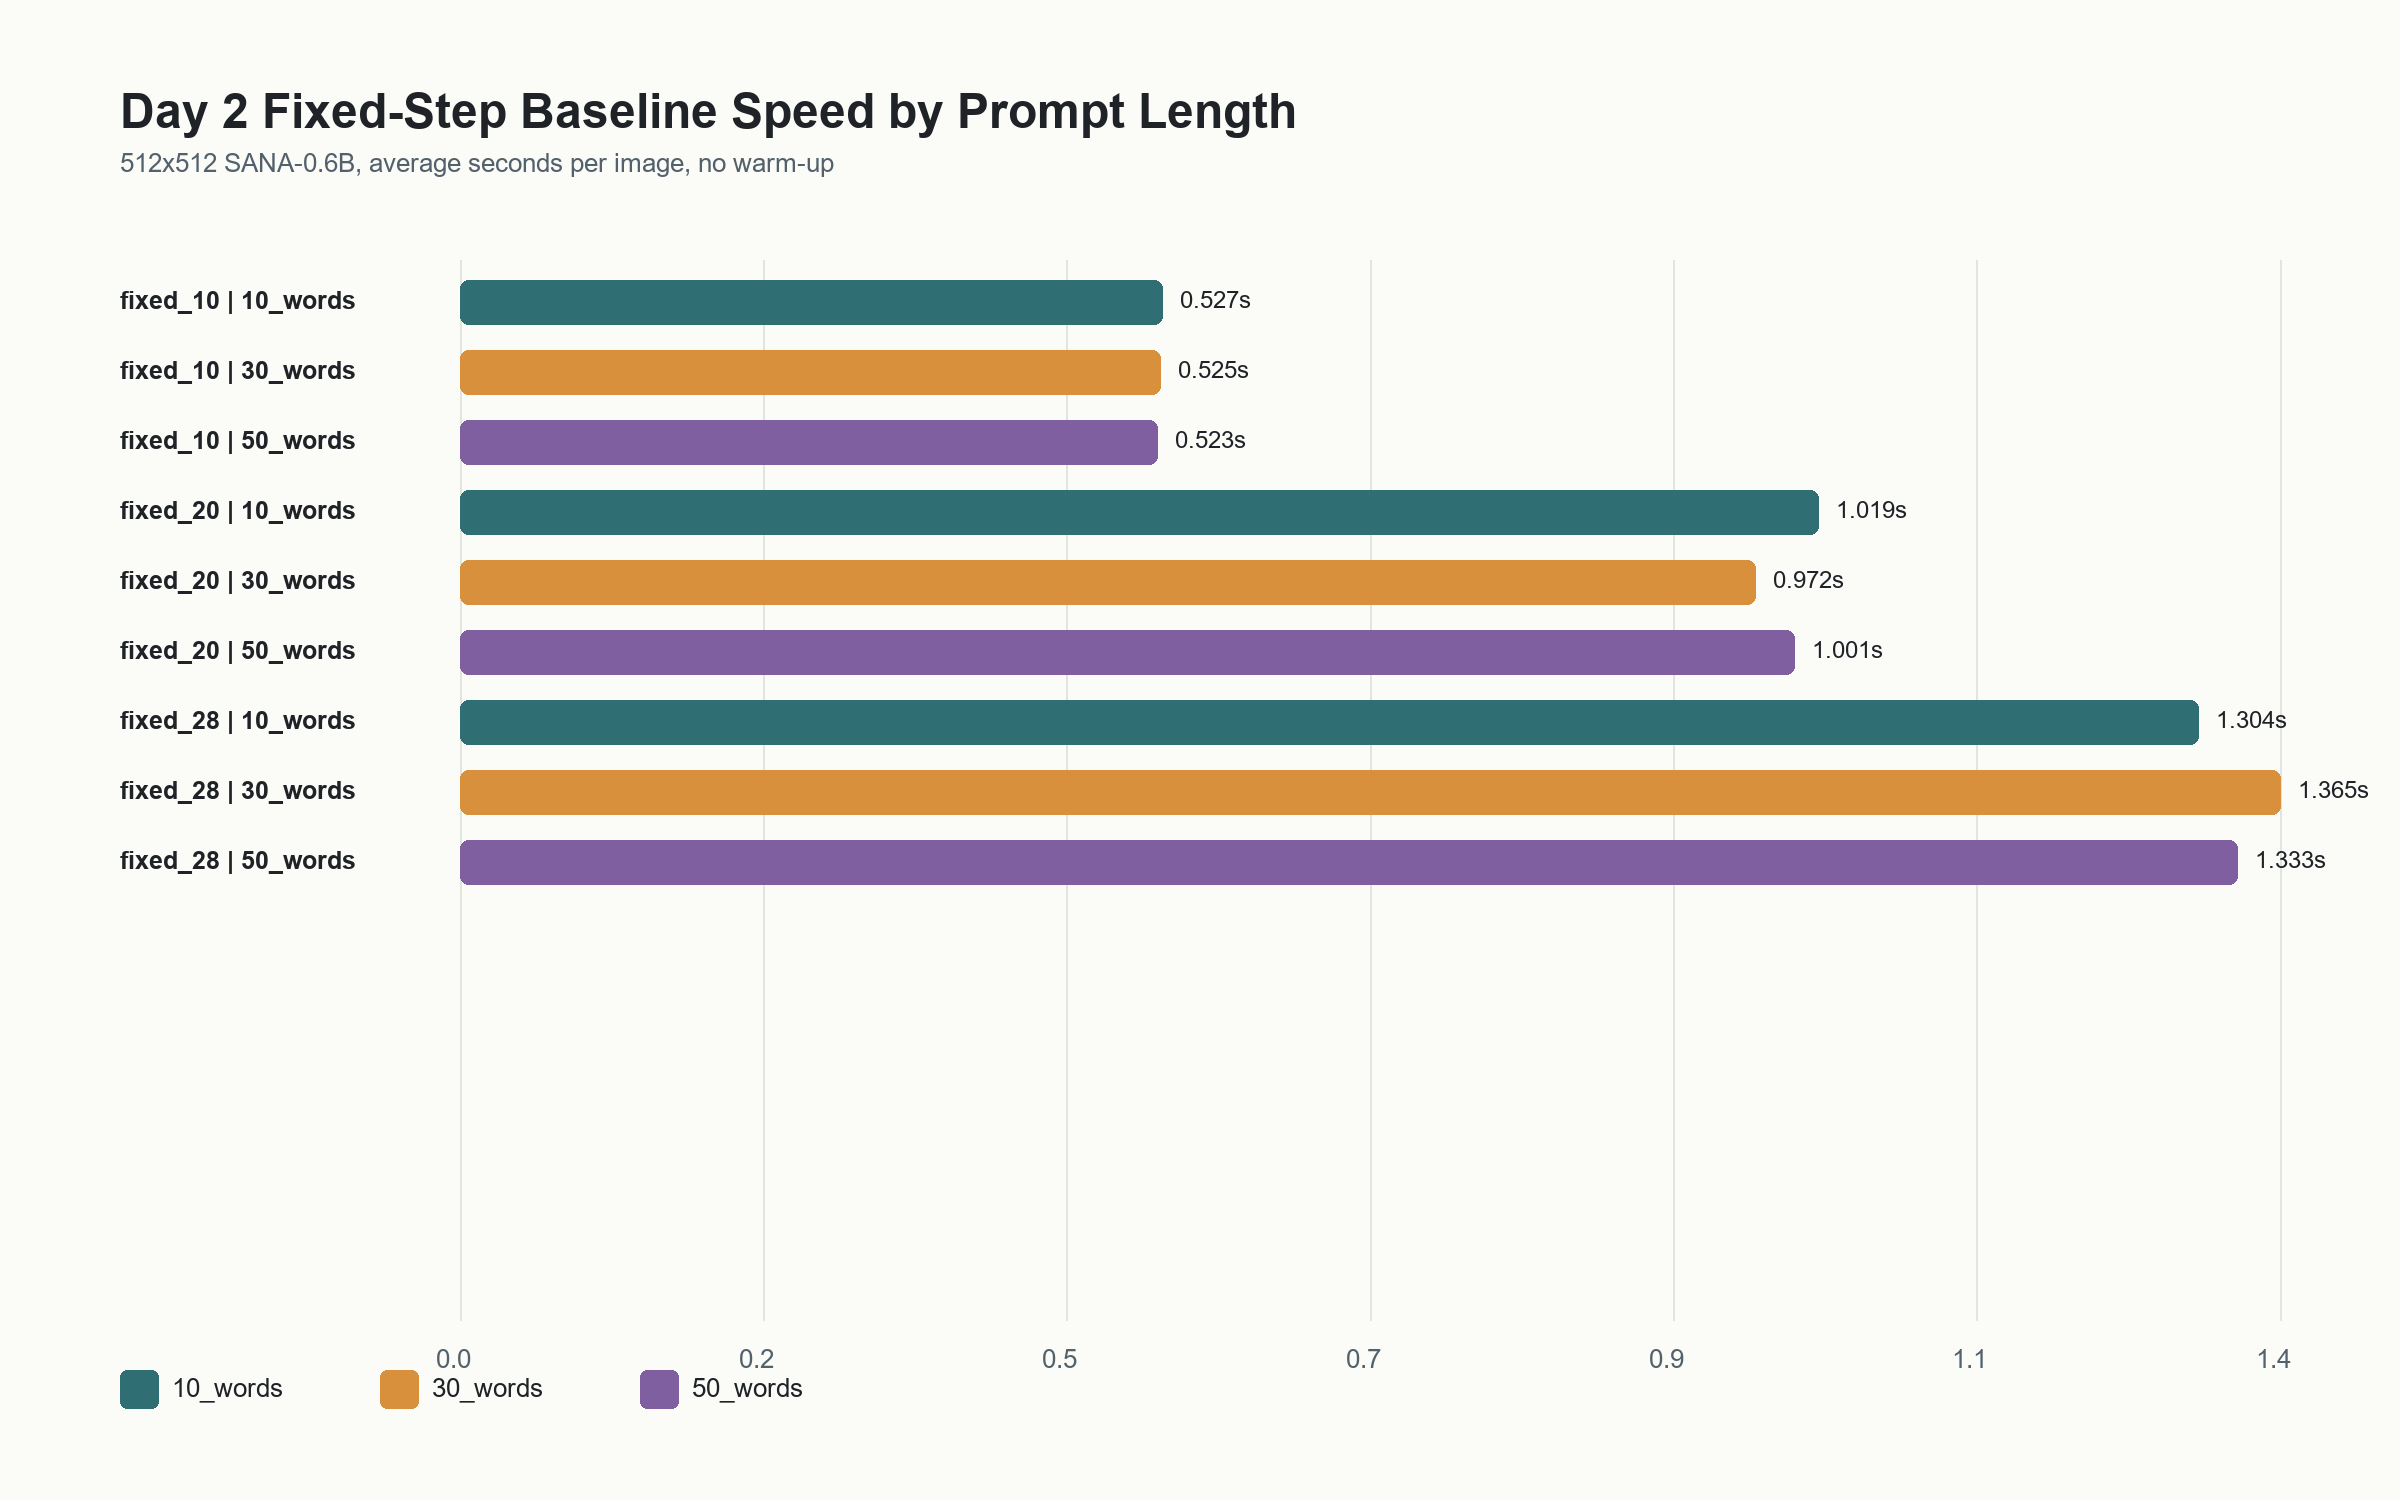
\includegraphics[width=0.86\linewidth]{day2_speed_summary_chart.png}
  \caption{Fixed-10、Fixed-20 与 Fixed-28 的平均推理时间比较。}
  \label{fig:day2_speed}
\end{figure}

这一结果给出 PCAS 的直接动机：增加采样步数确实可能带来轻微自动对齐收益，但其边际收益明显小于时间开销增长。若所有 prompt 均使用同一预算，简单 prompt 上的冗余计算会被系统性保留，而复杂 prompt 也无法获得经过校准的额外资源。PCAS 因此关注 SANA 推理阶段的预算分配，而非替代 SANA backbone 本身。

\subsection{原始 Rule-PCAS：计算重分配有效但整体收益不足}

原始 Rule-PCAS 将 10-word prompt 映射到 10 steps，将 30-word prompt 映射到 20 steps，将 50-word prompt 映射到 28 steps。它符合“简单 prompt 少给 steps、复杂 prompt 多给 steps”的直觉，也确实在短 prompt 上带来明显加速：10-word 组相对 Fixed-20 节省约 41.8\% 时间。

然而，在当前 benchmark 中三组 prompt 各 10 条，50-word 组的 28 steps 会显著增加长 prompt 耗时。短 prompt 的节省被长 prompt 的额外开销抵消后，Rule-PCAS 全部 30 条 prompt 的平均时间仅从 0.996s 降至 0.977s，整体加速约 1.9\%。这说明原始 Rule-PCAS 更像是一种“计算重分配”策略，而不是严格意义上的整体加速策略。

该结果表明，长度分组能够提供可解释的复杂度代理，却不能单独保证有效的推理加速。一方面，词数并不等价于生成难度；另一方面，若不显式控制全局平均预算，复杂 prompt 的额外 steps 会吞掉短 prompt 的节省。因此，后续策略需要在保留 prompt-aware 分配能力的同时，将平均预算纳入 policy 设计。

\begin{figure}[H]
  \centering
  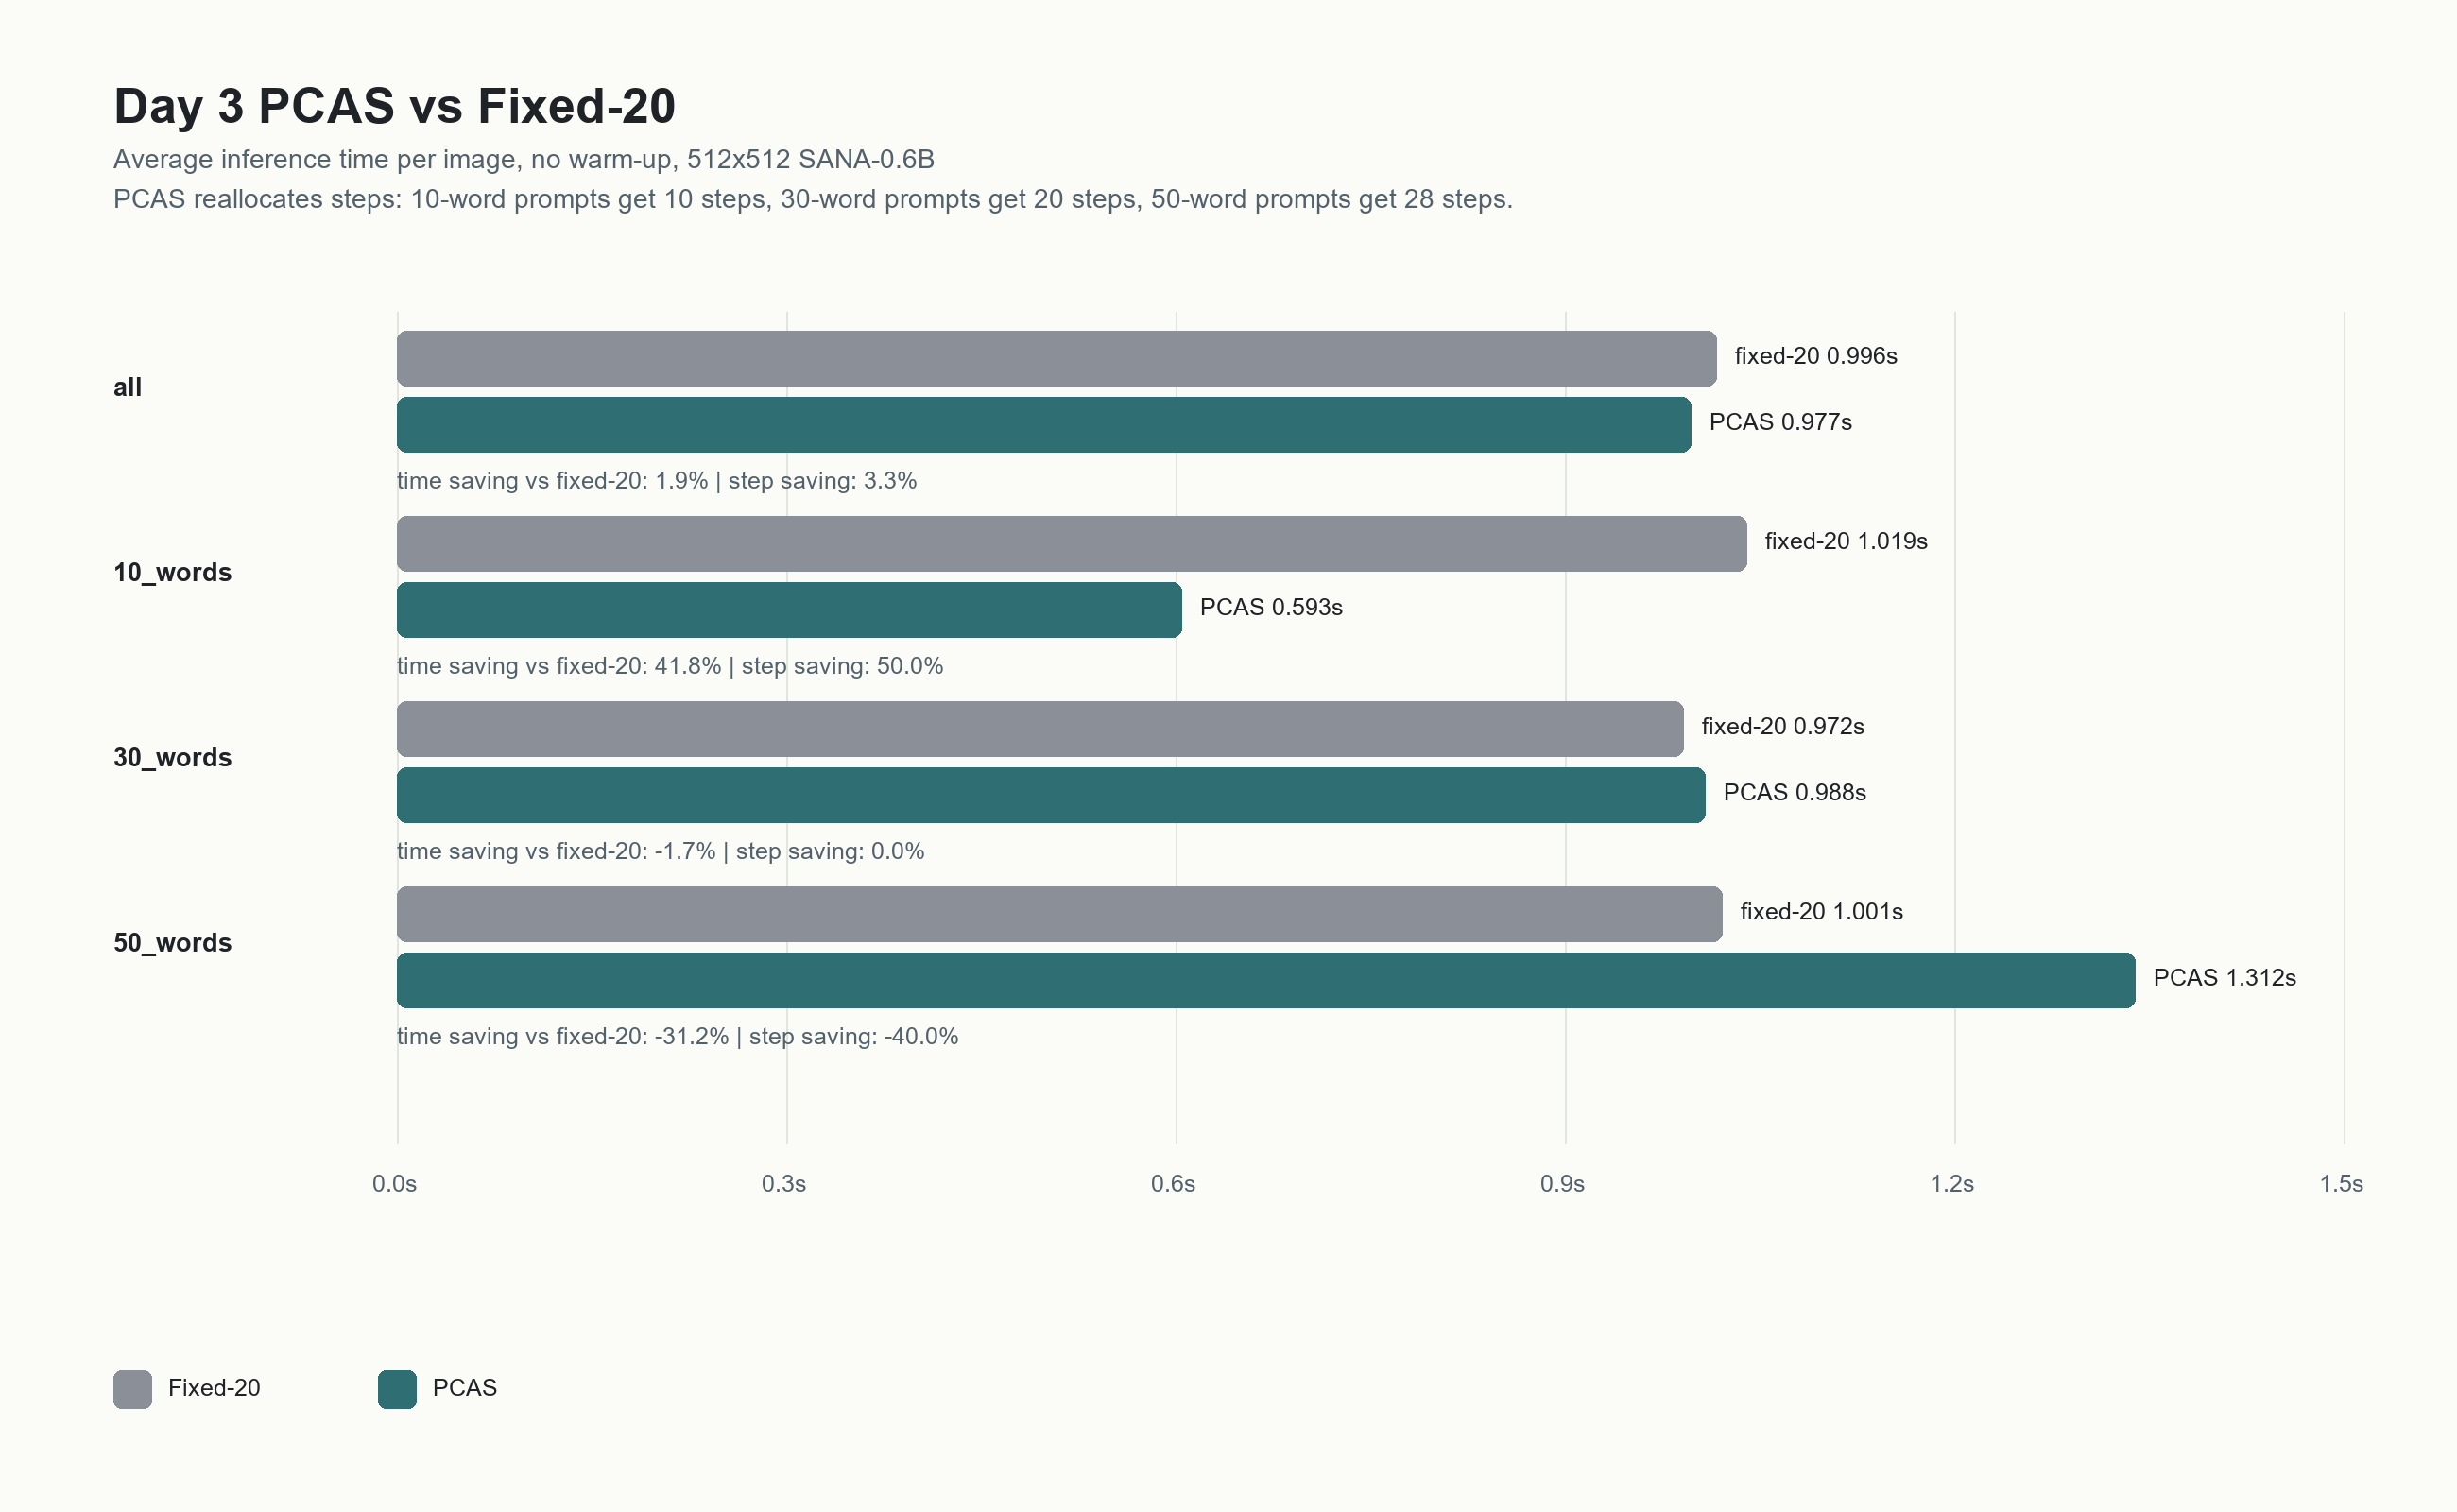
\includegraphics[width=0.82\linewidth]{day3_pcas_vs_fixed20_chart.png}
  \caption{原始 Rule-PCAS 与 Fixed-20 的时间对比。Rule-PCAS 在短 prompt 上收益明显，但长 prompt 的额外 steps 抵消了整体收益。}
  \label{fig:rule_pcas}
\end{figure}

\subsection{Balanced-PCAS：相对于固定 SANA 推理的主要效率优势}

Balanced-PCAS 在 Rule-PCAS 的观察基础上加入显式预算约束。它保留 prompt-aware 的分组思想，但不再让长 prompt 直接升到 28 steps，而是使用 8/16/24 steps 的策略。这样，短 prompt 获得更充分的时间节省，中等 prompt 也低于 Fixed-20，长 prompt 虽然仍略高于 20 steps，但相比 Rule-PCAS 的 28 steps 明显收敛。Balanced-PCAS 的核心不在于修改 SANA 结构，而在于将“按复杂度重分配计算”转化为“在平均预算下降前提下重分配计算”。

\begin{table}[H]
  \centering
  \caption{Rule-PCAS 与 Balanced-PCAS 的策略比较}
  \label{tab:balanced_policy}
  \begin{tabular}{lrrrr}
    \toprule
    Prompt 组 & Rule-PCAS steps & Rule guidance & Balanced steps & Balanced guidance \\
    \midrule
    10-word & 10 & 4.0 & 8  & 4.0 \\
    30-word & 20 & 4.5 & 16 & 4.4 \\
    50-word & 28 & 5.0 & 24 & 4.8 \\
    \bottomrule
  \end{tabular}
\end{table}

\begin{table}[H]
  \centering
  \caption{Balanced-PCAS 相对 Fixed-20 的主结果}
  \label{tab:balanced_main}
  \small
  \resizebox{0.98\linewidth}{!}{%
  \begin{tabular}{lrrrr}
    \toprule
    方法 & 平均 steps & 去预热平均时间(s) & 相对 Fixed-20 时间节省 & 平均 \clipscore{} \\
    \midrule
    Fixed-20 & 20.000 & 0.996 & 0.0\% & 35.762 \\
    Rule-PCAS & 19.333 & 0.977 & 1.9\% & 35.750 \\
    Balanced-PCAS & 16.000 & 0.751 & 24.6\% & 35.772 \\
    \bottomrule
  \end{tabular}}
\end{table}

\begin{figure}[H]
  \centering
  \begin{subfigure}{0.48\linewidth}
    \centering
    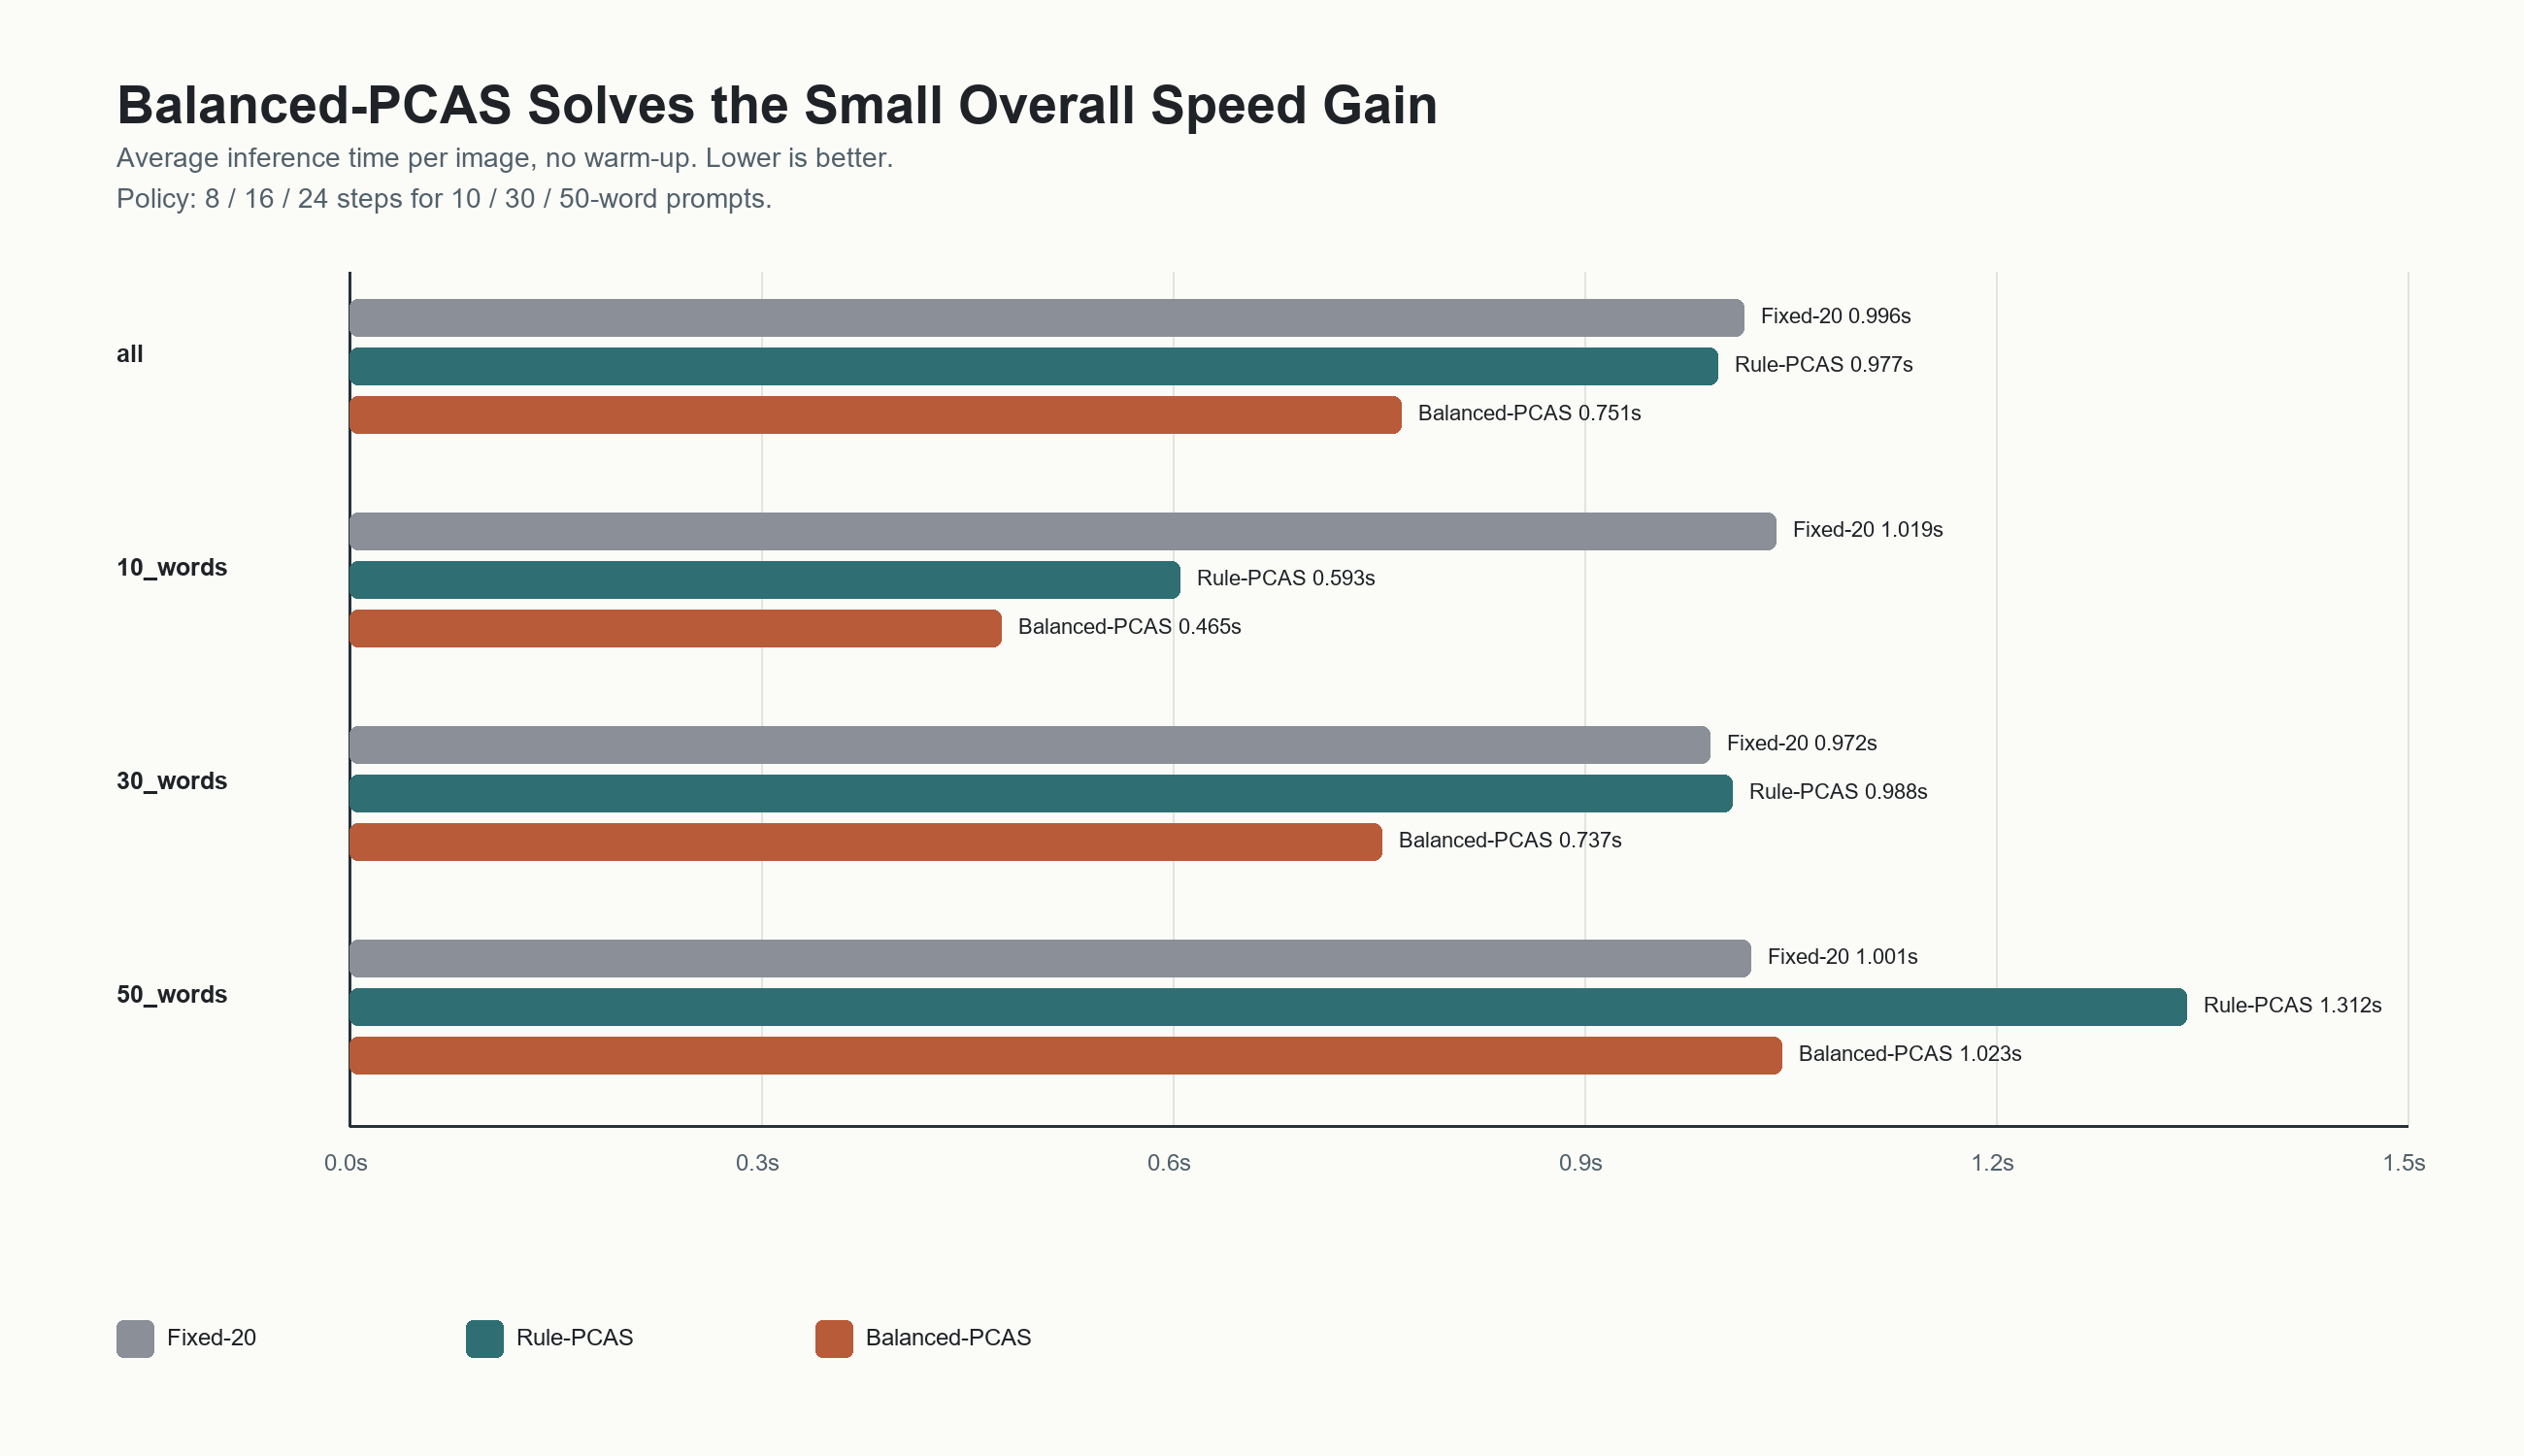
\includegraphics[width=\linewidth]{day3_pcas_balanced_speed_chart.png}
    \caption{平均时间对比}
  \end{subfigure}
  \hfill
  \begin{subfigure}{0.48\linewidth}
    \centering
    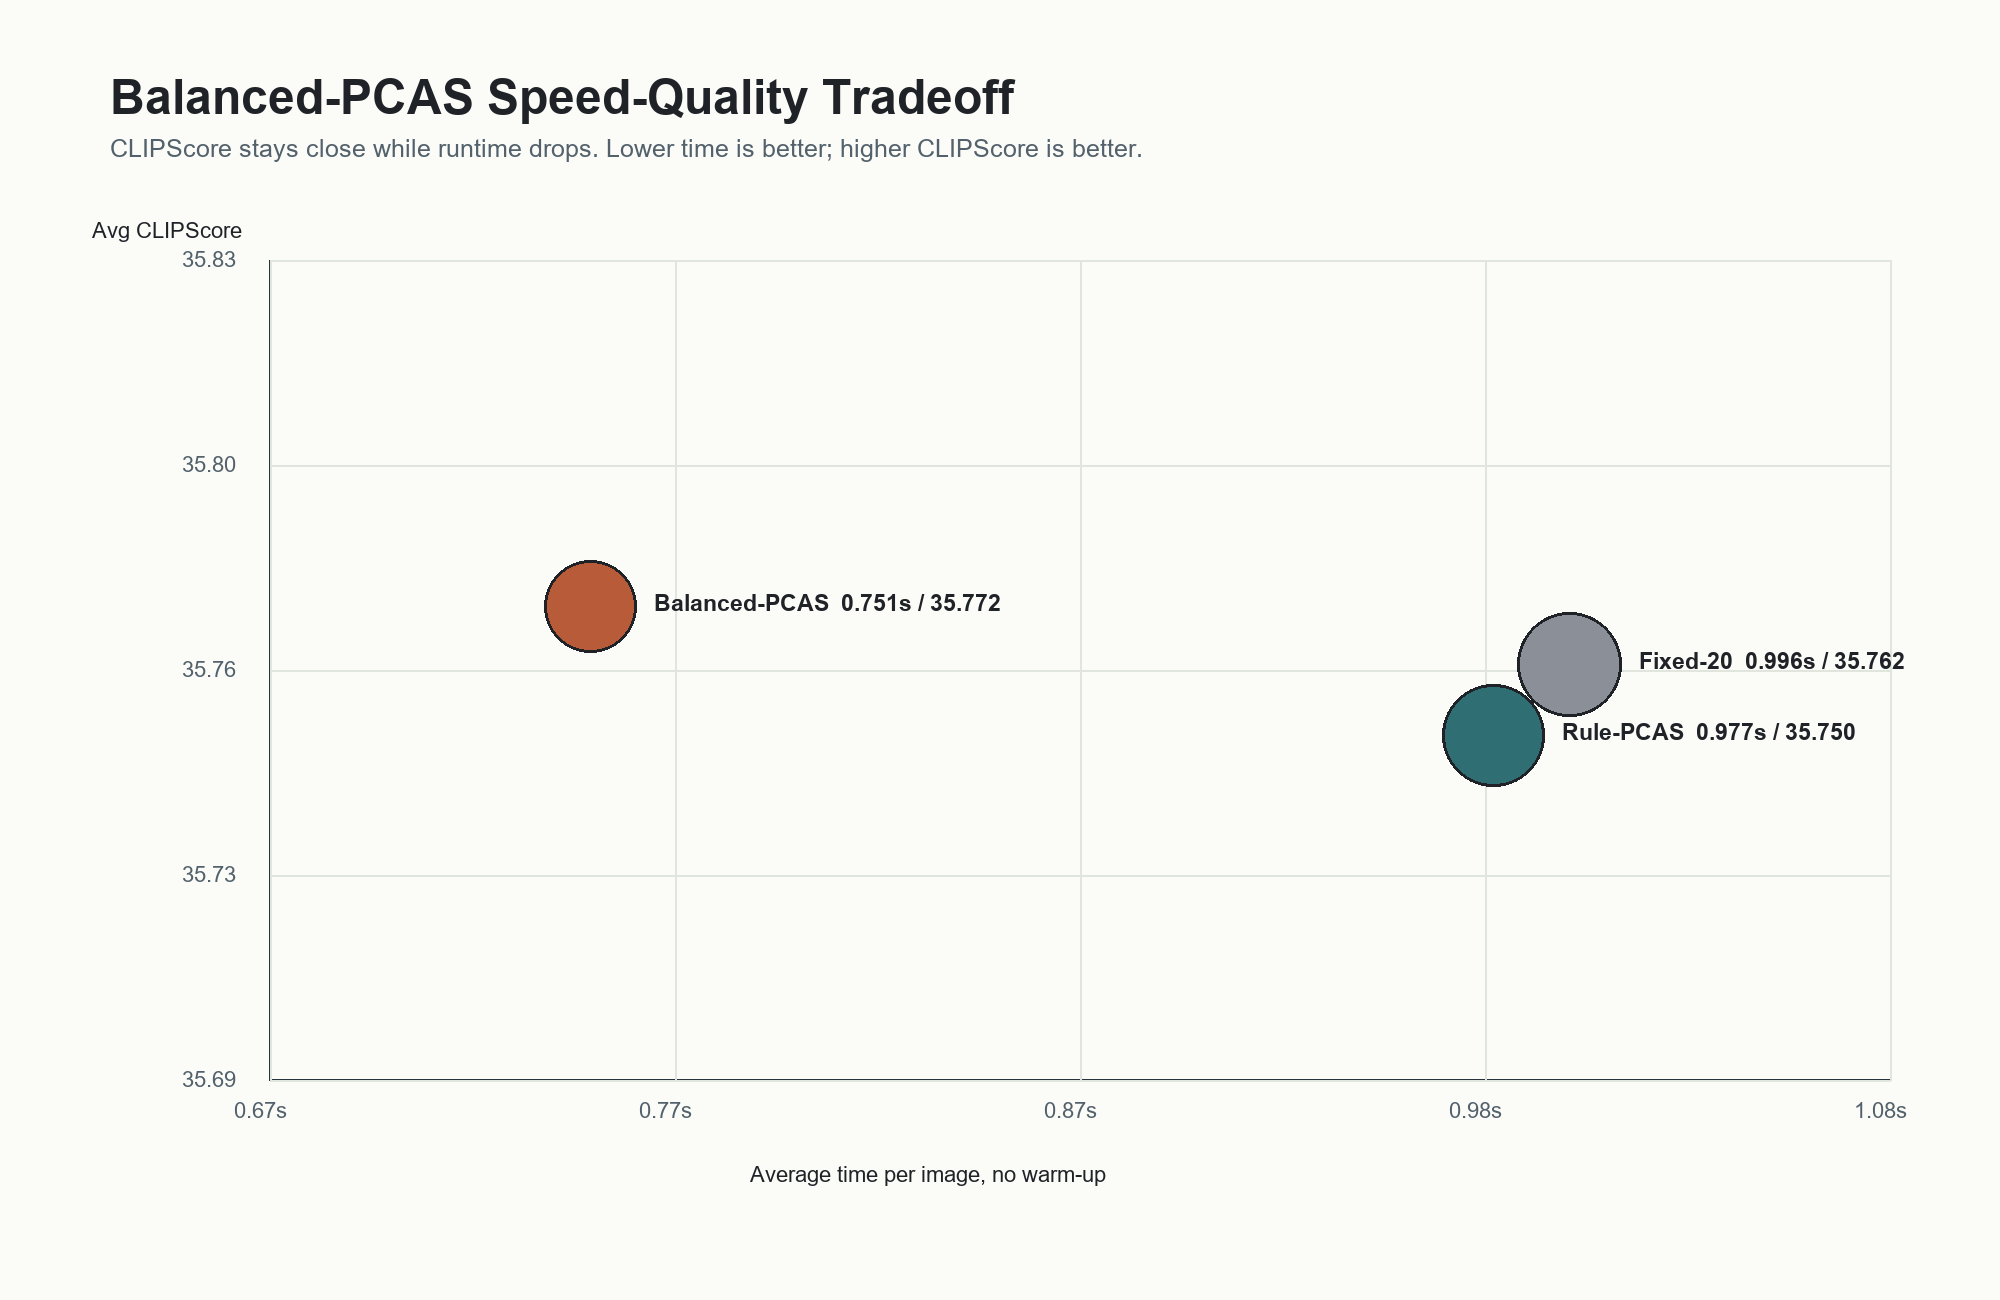
\includegraphics[width=\linewidth]{day3_pcas_balanced_speed_quality_tradeoff.png}
    \caption{速度--质量权衡}
  \end{subfigure}
  \caption{Balanced-PCAS 的主结果。相对于原始 SANA 的 Fixed-20 推理，Balanced-PCAS 显著降低平均时间，同时保持 \clipscore{} 接近。}
  \label{fig:balanced}
\end{figure}

\cref{tab:balanced_main} 与 \cref{fig:balanced} 表明，Balanced-PCAS 是本文最主要的效率成果。相对于直接使用原始 SANA 固定 20-step 推理，它将平均 steps 从 20 降为 16，将去预热平均时间从 0.996s 降为 0.751s，获得约 24.6\% 的平均加速。与此同时，平均 \clipscore{} 从 35.762 变为 35.772，差异可以视为同一水平。由此可见，PCAS 并不是提升 SANA 生成能力本身，而是使 SANA 的计算预算更符合 prompt 难度。

因此，Balanced-PCAS 说明自适应采样必须同时满足 prompt-aware 与 budget-aware 两个条件。没有预算约束时，策略可能只是把短 prompt 省下的时间转移给长 prompt；加入预算约束后，PCAS 才形成相对于 Fixed-20 的稳定效率优势。

\subsection{DeepSeek-Balanced：从语义复杂度到预算约束调度}

DeepSeek-assisted PCAS 的目标是让复杂度估计不只依赖词数。前一阶段的规则分组虽然可复现，但无法区分“短而难”的文字渲染 prompt、带稀有概念的 prompt，以及“长而简单”的冗长描述。为补足这一点，DeepSeek 会根据对象数量、关系数量、风格约束和文字生成需求输出 low、medium 或 high 标签。在当前 30 条 benchmark 中，DeepSeek 将 5 条判为 low，6 条判为 medium，19 条判为 high。这个结果说明 LLM 倾向于从语义角度更保守地看待 prompt，尤其是 30-word 和 50-word 组中包含场景、角色和风格约束的 prompt。

原始 DeepSeek-PCAS 使用 low/medium/high=10/20/28 steps，因此 high 标签过多会导致平均 steps 达到 23.4，平均时间为 1.303s，比 Fixed-20 慢 30.8\%。这一结果并不否定 DeepSeek 标签的语义信息，而是表明标签到动作的 policy 过于激进：LLM 对“语义复杂”的判断不能直接等同于“需要更多 steps”。DeepSeek-Balanced 复用同一批标签，但将策略改为 8/16/22 steps，使 LLM 复杂度判断变成预算约束下的语义调度。

\begin{table}[H]
  \centering
  \caption{DeepSeek-PCAS 与 DeepSeek-Balanced 的速度和质量对比}
  \label{tab:deepseek_main}
  \small
  \makebox[\linewidth][c]{%
  \resizebox{0.96\linewidth}{!}{%
  \begin{tabular}{@{}lrrrrr@{}}
    \toprule
    方法 & Low/Medium/High & 平均 steps & 去预热平均时间(s) & 时间节省 & 平均 \clipscore{} \\
    \midrule
    Fixed-20 & -- & 20.000 & 0.996 & 0.0\% & 35.762 \\
    DeepSeek-PCAS & 5/6/19 & 23.400 & 1.303 & -30.8\% & 35.829 \\
    DeepSeek-Balanced & 5/6/19 & 18.467 & 0.844 & 15.3\% & 35.813 \\
    \bottomrule
  \end{tabular}}}
\end{table}

\begin{figure}[H]
  \centering
  \begin{subfigure}{0.48\linewidth}
    \centering
    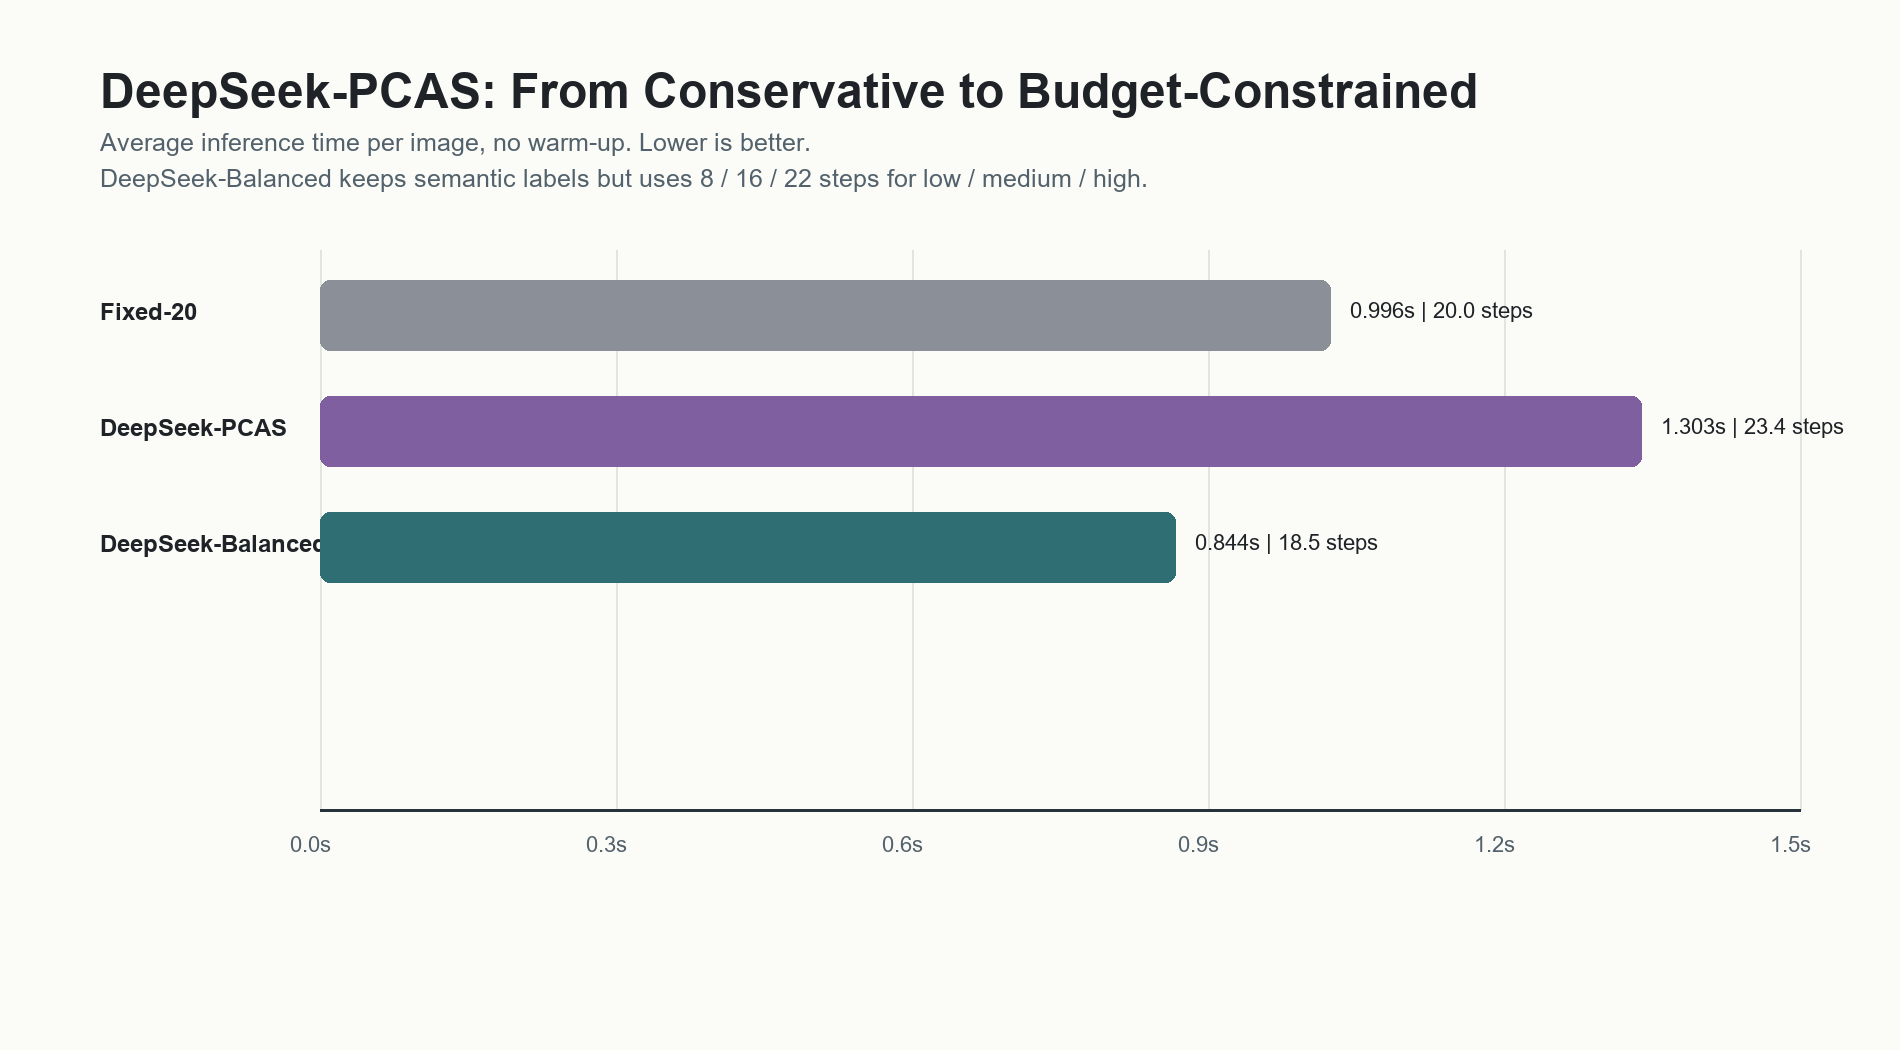
\includegraphics[width=\linewidth]{day3_deepseek_balanced_speed_chart.png}
    \caption{平均时间对比}
  \end{subfigure}
  \hfill
  \begin{subfigure}{0.48\linewidth}
    \centering
    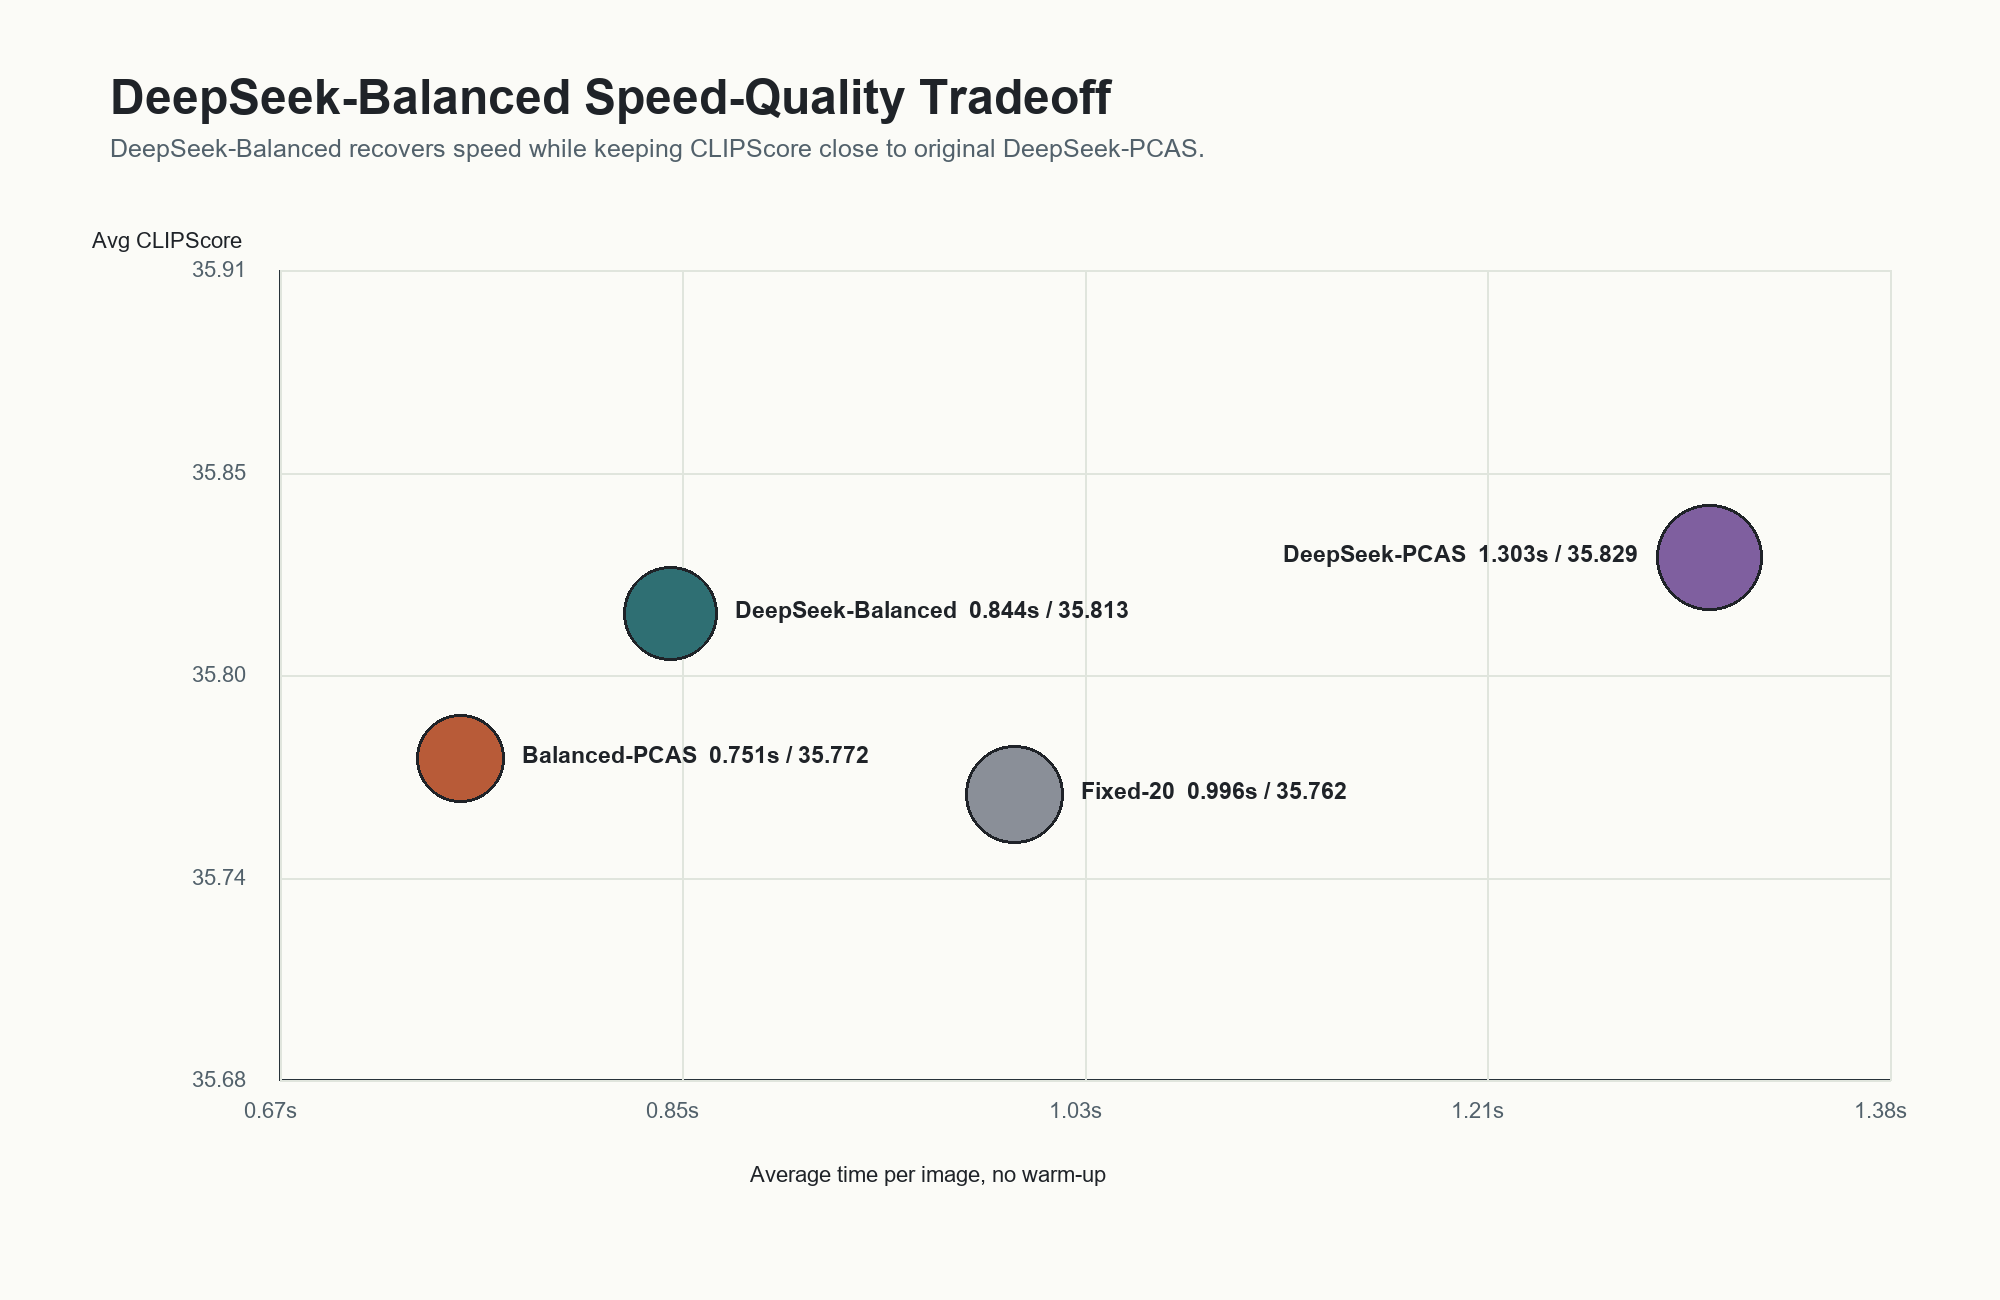
\includegraphics[width=\linewidth]{day3_deepseek_balanced_speed_quality_tradeoff.png}
    \caption{速度--质量权衡}
  \end{subfigure}
  \caption{DeepSeek-Balanced 将 LLM 语义复杂度标签转化为预算约束下的推理调度。}
  \label{fig:deepseek_balanced}
\end{figure}

DeepSeek-Balanced 的意义在于，它展示了 PCAS 不必局限于词数规则。更丰富的语义复杂度标签可以进入同一套 adaptive policy，但必须经过预算校准。若直接将 high 语义复杂度映射到过高 steps，策略会变成质量保守、延迟增加；若在预算约束下使用语义标签，则可以兼顾 prompt 难度排序与整体效率。由此可见，复杂度估计与采样动作应被视为两个相互连接但并不等价的模块：前者描述输入难度，后者在延迟约束下选择资源分配。

\subsection{Calibrated-PCAS：从手工规则到数据校准 policy}

Balanced-PCAS 和 DeepSeek-Balanced 解决了平均预算问题，但二者仍属于手工 policy：8/16/24 或 8/16/22 的选择可以解释，却没有直接回答每条 prompt 究竟需要多少 steps 才能接近 Fixed-20。为将自适应采样转化为具有明确约束目标的预测问题，本文构建 calibration dataset。对 30 条 benchmark prompt 分别在 8、12、16、20、24 和 28 steps 下生成图像，固定 guidance=4.5，并计算每张图像的 \clipscore{}。以 Fixed-20 为参考，取 $\epsilon=0.2$ 定义最小充分 steps 标签。标签分布见 \cref{tab:calibration_labels}。

\begin{table}[H]
  \centering
  \caption{Calibrated-PCAS 的最小充分 steps 标签分布}
  \label{tab:calibration_labels}
  \begin{tabular}{rr}
    \toprule
    最小充分 steps & Prompt 数量 \\
    \midrule
    8 & 18 \\
    12 & 4 \\
    16 & 6 \\
    20 & 2 \\
    \bottomrule
  \end{tabular}
\end{table}

在当前 benchmark 和 \clipscore{} 容忍阈值下，多数 prompt 不需要完整 20 steps 即可达到 Fixed-20 附近的自动文本对齐指标。随后本文分别训练 rule-feature decision tree 和 LLM-feature decision tree。Rule-feature 版本只使用本地解析特征，包括对象数、属性数、空间关系、文字渲染需求、场景密度和稀有概念等；LLM-feature 版本调用 DeepSeek 输出结构化 JSON 特征。在 30 条 prompt 上，DeepSeek 给出的 difficulty 分布为 low=10、medium=7、high=13，说明 LLM 特征比单纯词数更关注场景密度和语义复杂度。

\begin{table}[H]
  \centering
  \caption{Calibrated-PCAS 与已有策略的对比}
  \label{tab:calibrated_main}
  \small
  \makebox[\linewidth][c]{%
  \resizebox{0.98\linewidth}{!}{%
  \begin{tabular}{@{}lrrrrr@{}}
    \toprule
    方法 & 平均 steps & 时间(s) & 相对 Fixed-20 & 平均 \clipscore{} & 约束满足率 \\
    \midrule
    Fixed-20 & 20.000 & 1.537 & 0.0\% & 35.762 & 100.0\% \\
    Balanced-PCAS & 16.000 & 1.740 & -13.2\% & 35.772 & 73.3\% \\
    DeepSeek-Balanced & 18.467 & 2.023 & -31.6\% & 35.813 & 73.3\% \\
    Oracle minimum & 10.933 & 1.112 & 27.6\% & 36.276 & 100.0\% \\
    Calibrated-PCAS & 10.667 & 0.675 & 56.1\% & 36.234 & 96.7\% \\
    LLM-feature Calibrated-PCAS & 11.333 & 1.093 & 28.9\% & 36.230 & 96.7\% \\
    \bottomrule
  \end{tabular}}}
\end{table}

\cref{tab:calibrated_main} 显示，Calibrated-PCAS 相比 Balanced-PCAS 和 DeepSeek-Balanced 更接近 oracle minimum：它显著降低平均 steps，并将逐 prompt 的 Fixed-20 约束满足率从 73.3\% 提升到 96.7\%。Rule-feature 和 LLM-feature 两个版本的平均 \clipscore{} 都约为 36.23，高于对应实验批次中 Fixed-20 的 35.76。由于 \clipscore{} 对 steps 的响应并不严格单调，这一结果不应被理解为“采样步数越少质量越高”；更合理的解释是，calibration policy 捕捉到了当前 benchmark 中最小充分预算的经验分布，从而在满足约束的同时节省 steps。

上述结果共同形成一条递进的证据链：Fixed baseline 揭示固定预算的边际收益有限；Rule-PCAS 证明 prompt-aware 分配可行，但也显示缺少平均预算约束会削弱整体收益；Balanced-PCAS 通过预算约束获得稳定加速；DeepSeek-Balanced 说明语义复杂度可以进入策略，但复杂度标签必须与采样动作校准；Calibrated-PCAS 则进一步将手工策略推进为“Fixed-20 质量约束下预测最小充分 steps”的可解释学习问题。

需要说明的是，Fixed-20、Balanced-PCAS、DeepSeek-Balanced 和 Calibrated-PCAS 的 wall-clock latency 会受到运行批次、系统负载和预热状态影响，因此不同实验批次的绝对时间不宜直接过度比较。Calibrated-PCAS 的更稳健证据是平均 steps 降低、\clipscore{} 约束满足率提升，以及 oracle minimum 与 learned policy 的距离较小；具体时间数字应结合运行环境解读。

\subsection{质量评价：PCAS 保持质量而非显著提高质量}

为评估采样策略是否影响文本--图像对齐，本文使用 CLIP ViT-B/32 计算 \clipscore{}。在全部 30 条 prompt 上，各方法之间的平均 \clipscore{} 差异很小。Fixed-10、Fixed-20、Fixed-28、Rule-PCAS、DeepSeek-PCAS 和 Balanced-PCAS 均处于 35.7--35.9 附近。采样步数增加带来轻微 \clipscore{} 提升，但幅度远小于推理时间的增加幅度。

\begin{table}[H]
  \centering
  \caption{主要方法在 30 条 prompt 上的速度--质量对比}
  \label{tab:quality_all}
  \begin{tabular}{lrrr}
    \toprule
    方法 & 平均 steps & 去预热平均时间(s) & 平均 \clipscore{} \\
    \midrule
    Fixed-10 & 10.000 & 0.525 & 35.689 \\
    Fixed-20 & 20.000 & 0.996 & 35.762 \\
    Fixed-28 & 28.000 & 1.335 & 35.890 \\
    Rule-PCAS & 19.333 & 0.977 & 35.750 \\
    DeepSeek-PCAS & 23.400 & 1.303 & 35.829 \\
    Balanced-PCAS & 16.000 & 0.751 & 35.772 \\
    \bottomrule
  \end{tabular}
\end{table}

\begin{figure}[H]
  \centering
  \begin{subfigure}{0.48\linewidth}
    \centering
    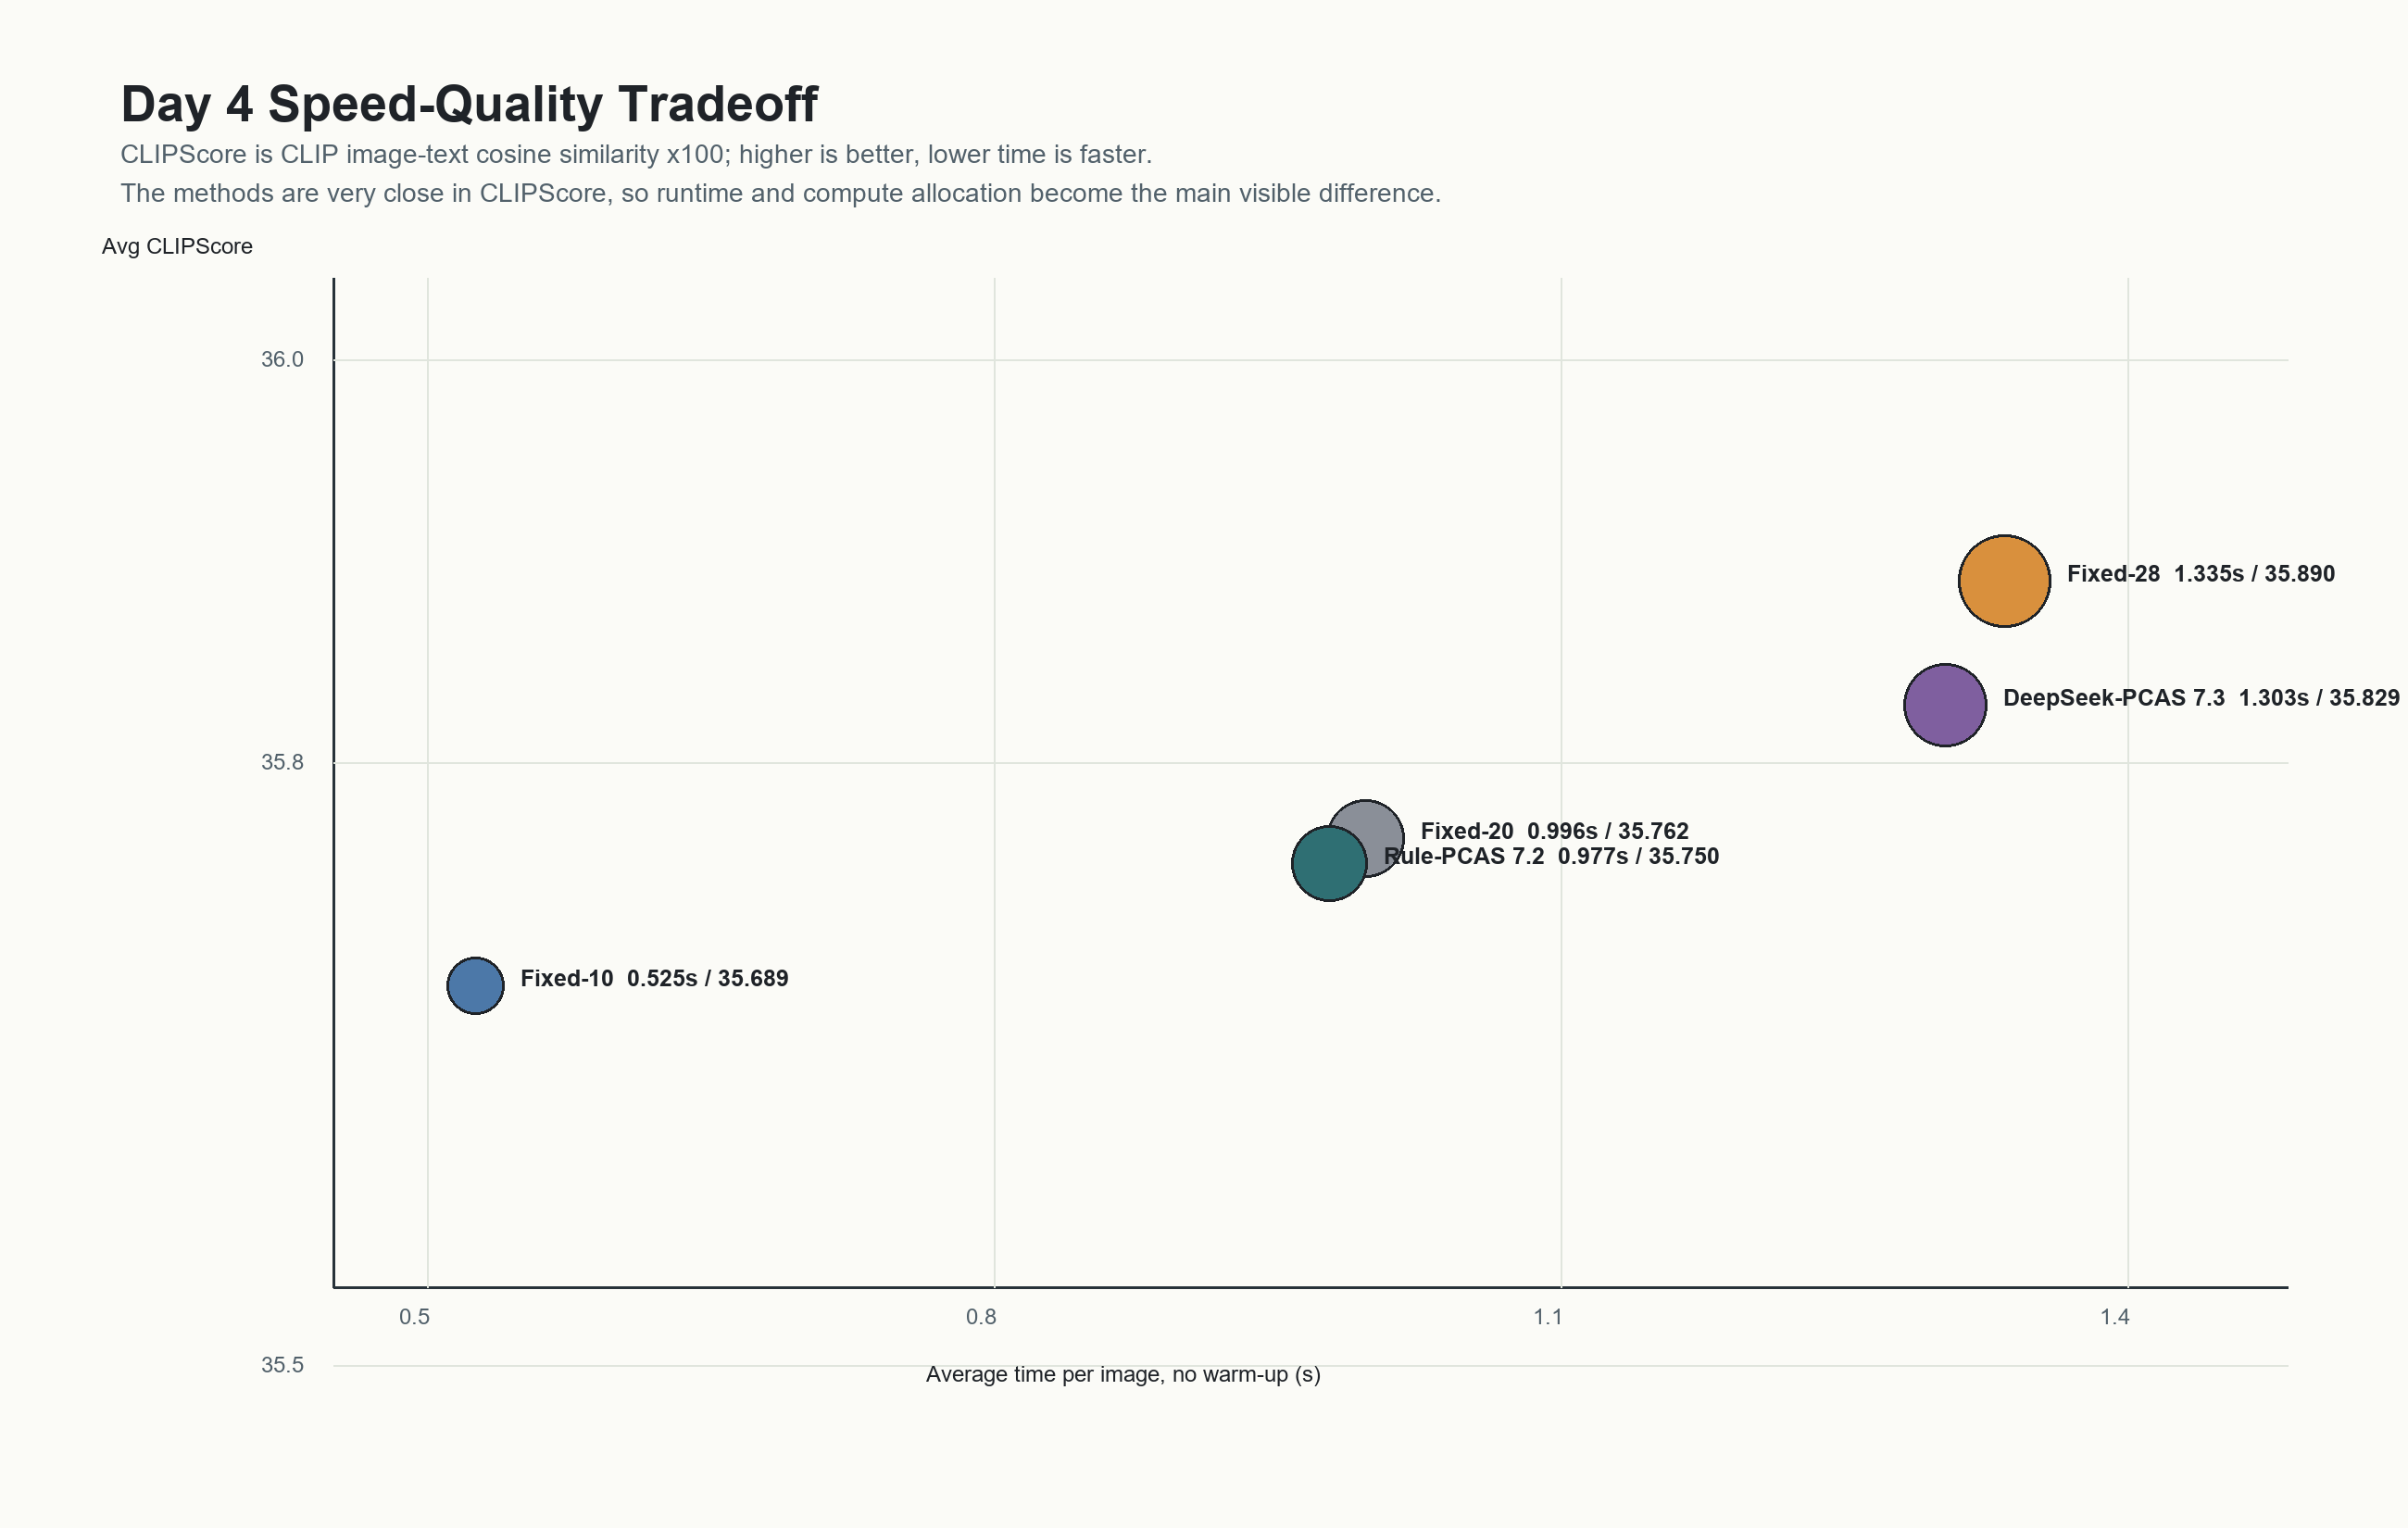
\includegraphics[width=\linewidth]{day4_speed_quality_tradeoff.png}
    \caption{整体速度--质量权衡}
  \end{subfigure}
  \hfill
  \begin{subfigure}{0.48\linewidth}
    \centering
    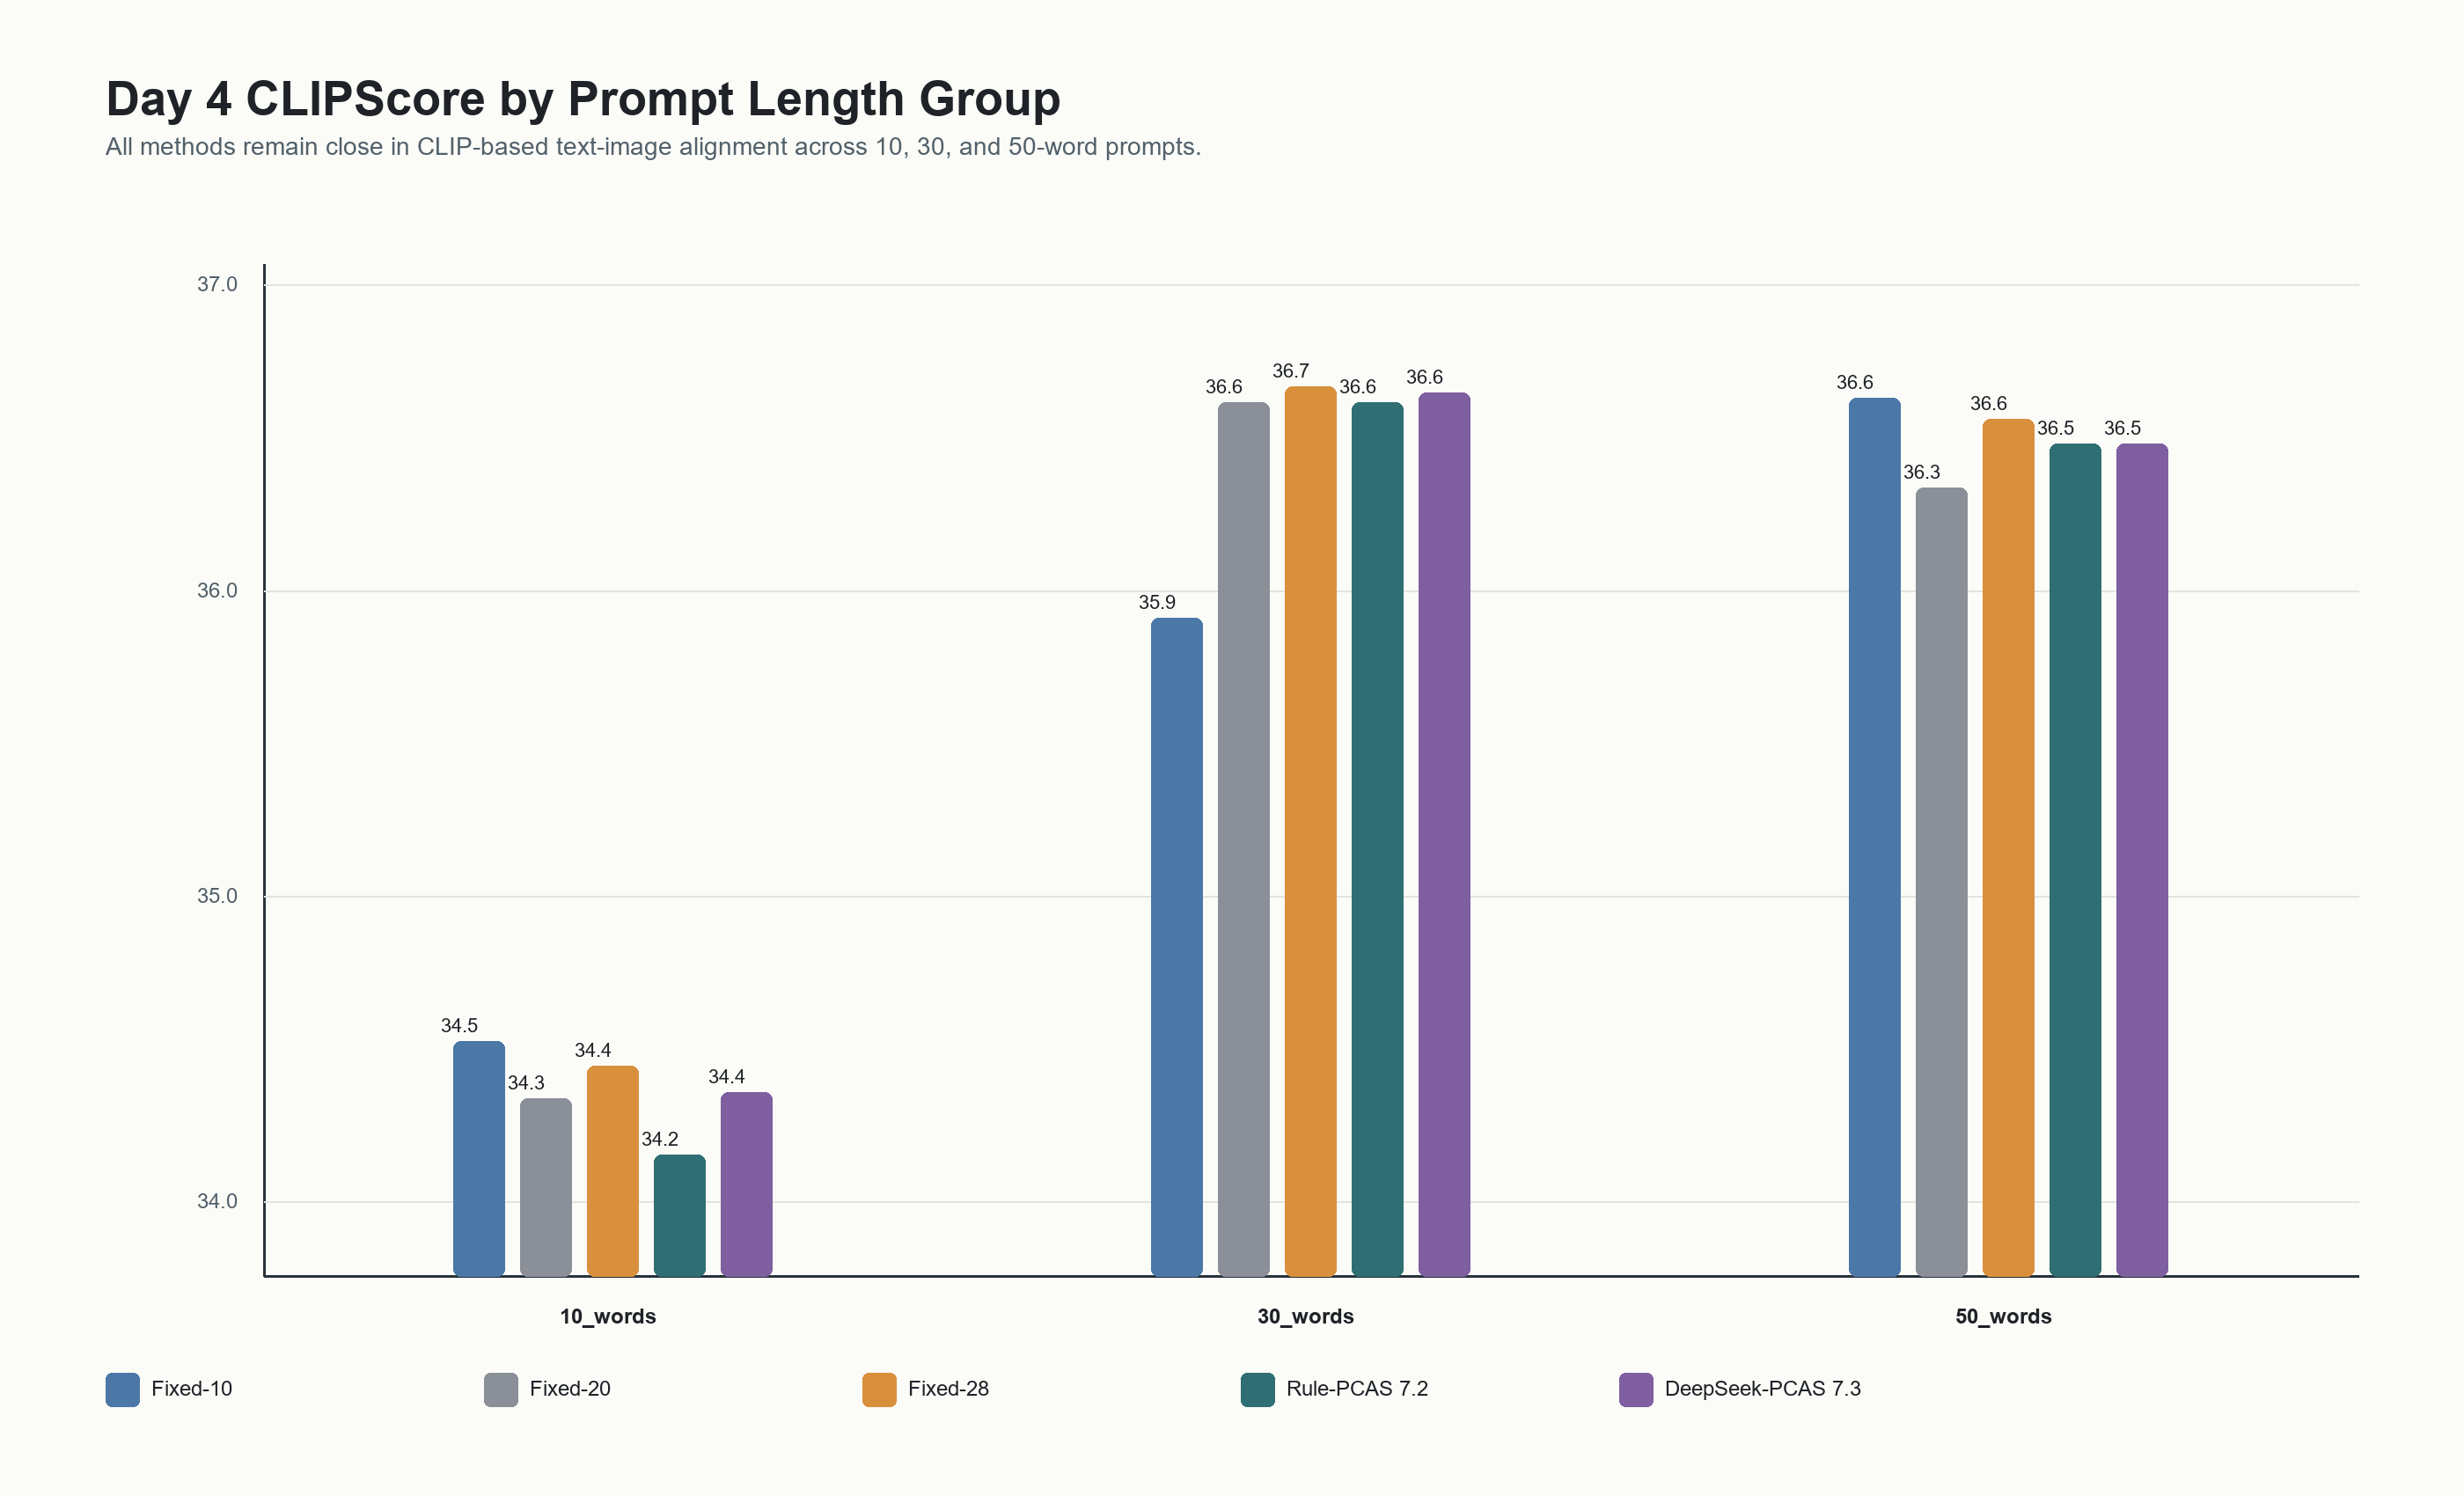
\includegraphics[width=\linewidth]{day4_clipscore_by_group.png}
    \caption{不同 prompt 组的 \clipscore{}}
  \end{subfigure}
  \caption{质量评价显示，各方法 \clipscore{} 差异较小；PCAS 更适合解释为效率--质量权衡优化。}
  \label{fig:day4_quality}
\end{figure}

因此，本文对质量结论采取审慎解释：现有证据并不支持 PCAS 能稳定提升图像质量；其主要价值在于以更低平均计算预算保持与固定 SANA 推理接近的自动语义对齐指标和视觉观感。这一边界有助于避免将小幅 \clipscore{} 波动过度解释为质量上限提升。

\subsection{Guidance scale 消融}

Guidance scale 控制文本条件对生成结果的影响强度。本文固定采样步数为 20，并测试 1.5、3.5、4.5、5.5、6.5 和 8.5。结果显示，3.5--6.5 的中等区间较为平稳，平均 \clipscore{} 范围仅约 0.130；guidance=1.5 明显降低文本对齐；guidance=8.5 给出最高平均 \clipscore{}，但这更可能反映 CLIP 对高 guidance 的轻微偏好，而不等价于视觉质量显著提升。

\begin{table}[H]
  \centering
  \caption{Guidance scale 消融实验}
  \label{tab:guidance}
  \begin{tabular}{rrrr}
    \toprule
    Guidance & 图像数 & 去预热平均时间(s) & 平均 \clipscore{} \\
    \midrule
    1.5 & 30 & 0.897 & 34.705 \\
    3.5 & 30 & 1.190 & 35.856 \\
    4.5 & 30 & 0.996 & 35.762 \\
    5.5 & 30 & 1.124 & 35.848 \\
    6.5 & 30 & 1.088 & 35.892 \\
    8.5 & 30 & 0.887 & 36.027 \\
    \bottomrule
  \end{tabular}
\end{table}

\begin{figure}[H]
  \centering
  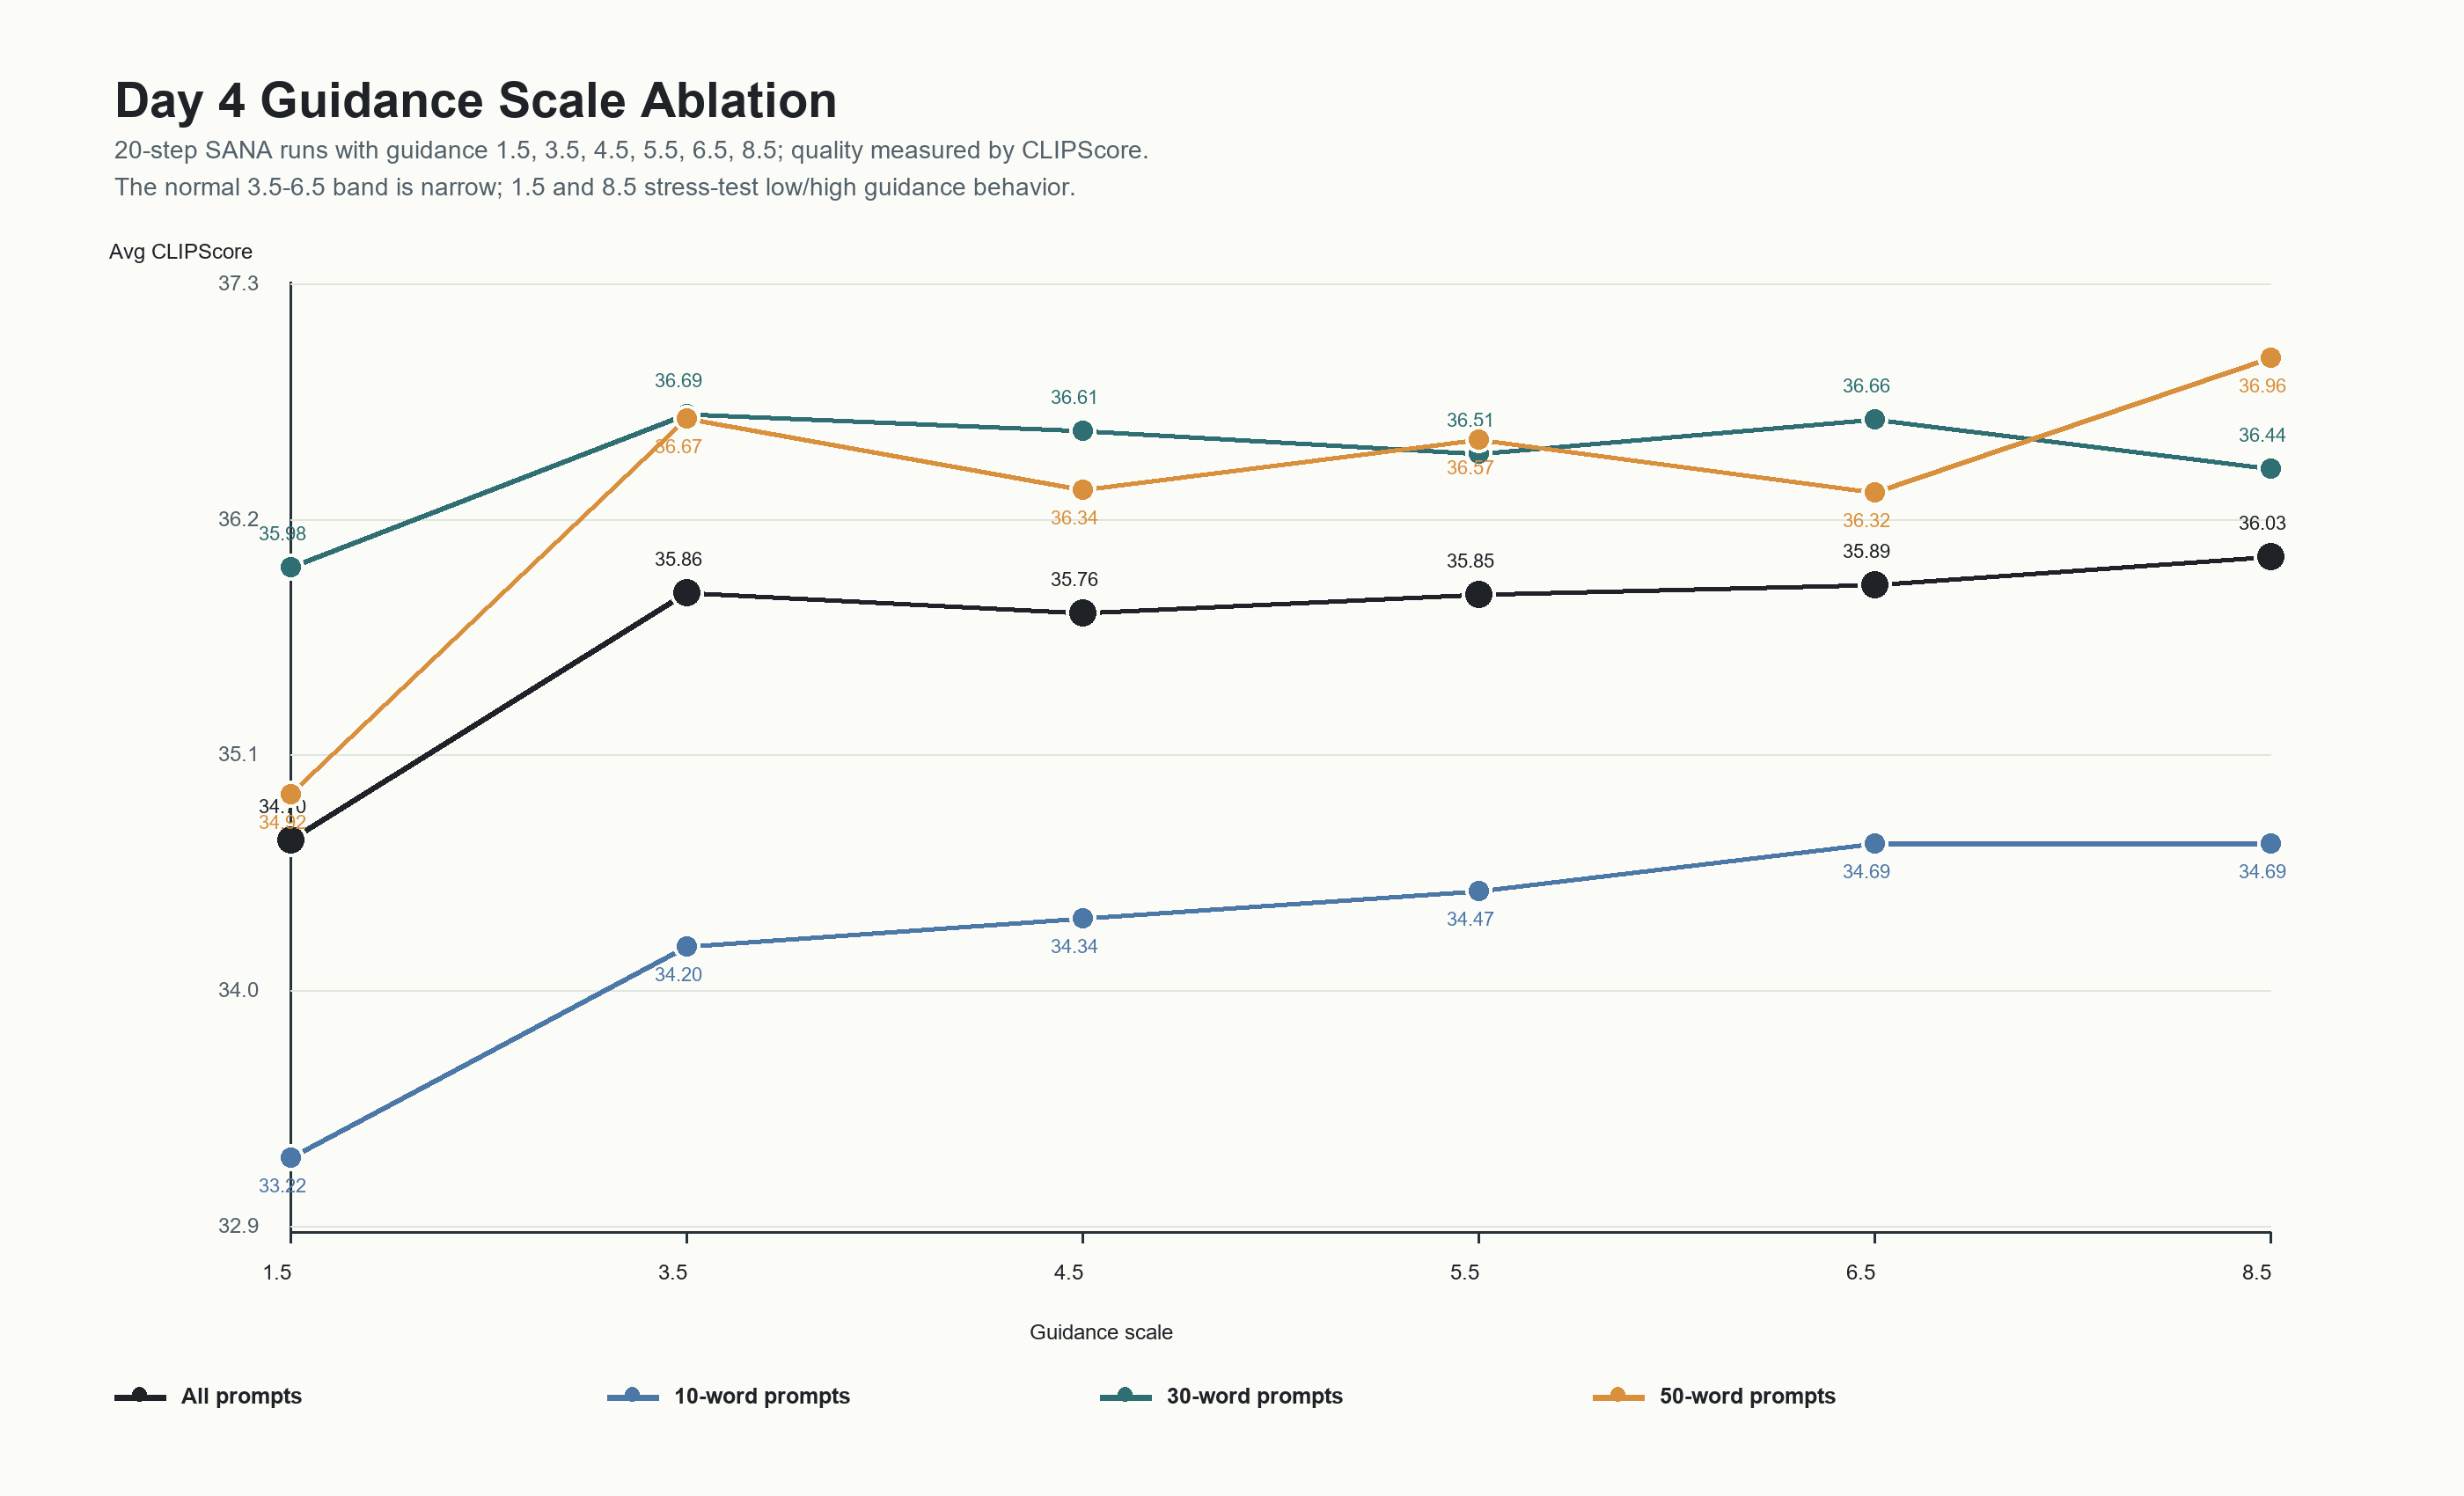
\includegraphics[width=0.86\linewidth]{day4_guidance_ablation_clipscore.png}
  \caption{Guidance scale 对平均 \clipscore{} 的影响。中等 guidance 区间较不敏感，低 guidance 明显削弱文本对齐。}
  \label{fig:guidance}
\end{figure}

这一结果说明，guidance 不是本文主线中最稳定的优化方向。默认 4.5 适合作为公平比较设置；若面向复杂 prompt 的自动语义对齐，可尝试更高 guidance，但需要同时检查视觉对比、局部细节和构图是否产生副作用。

\subsection{Hard prompt 定性分析与视觉差异}

为避免平均 \clipscore{} 掩盖复杂 prompt 中的细节问题，本文从 30 条 benchmark 中选出 8 条更困难的 prompt，覆盖复杂场景、多主体、多关系、文字生成和密集构图。比较方法包括 Fixed-20、Fixed-28、Rule-PCAS、Balanced-PCAS 和 DeepSeek-Balanced。

\begin{table}[H]
  \centering
  \caption{Hard prompt 子集上的自动指标}
  \label{tab:hard_prompt}
  \begin{tabular}{lrrrr}
    \toprule
    方法 & 图像数 & 平均 steps & 去预热平均时间(s) & 平均 \clipscore{} \\
    \midrule
    Fixed-20 & 8 & 20.000 & 0.978 & 36.522 \\
    Fixed-28 & 8 & 28.000 & 1.357 & 36.718 \\
    Rule-PCAS & 8 & 26.000 & 1.225 & 36.748 \\
    Balanced-PCAS & 8 & 22.000 & 0.953 & 36.526 \\
    DeepSeek-Balanced & 8 & 22.000 & 0.955 & 36.440 \\
    \bottomrule
  \end{tabular}
\end{table}

\begin{figure}[H]
  \centering
  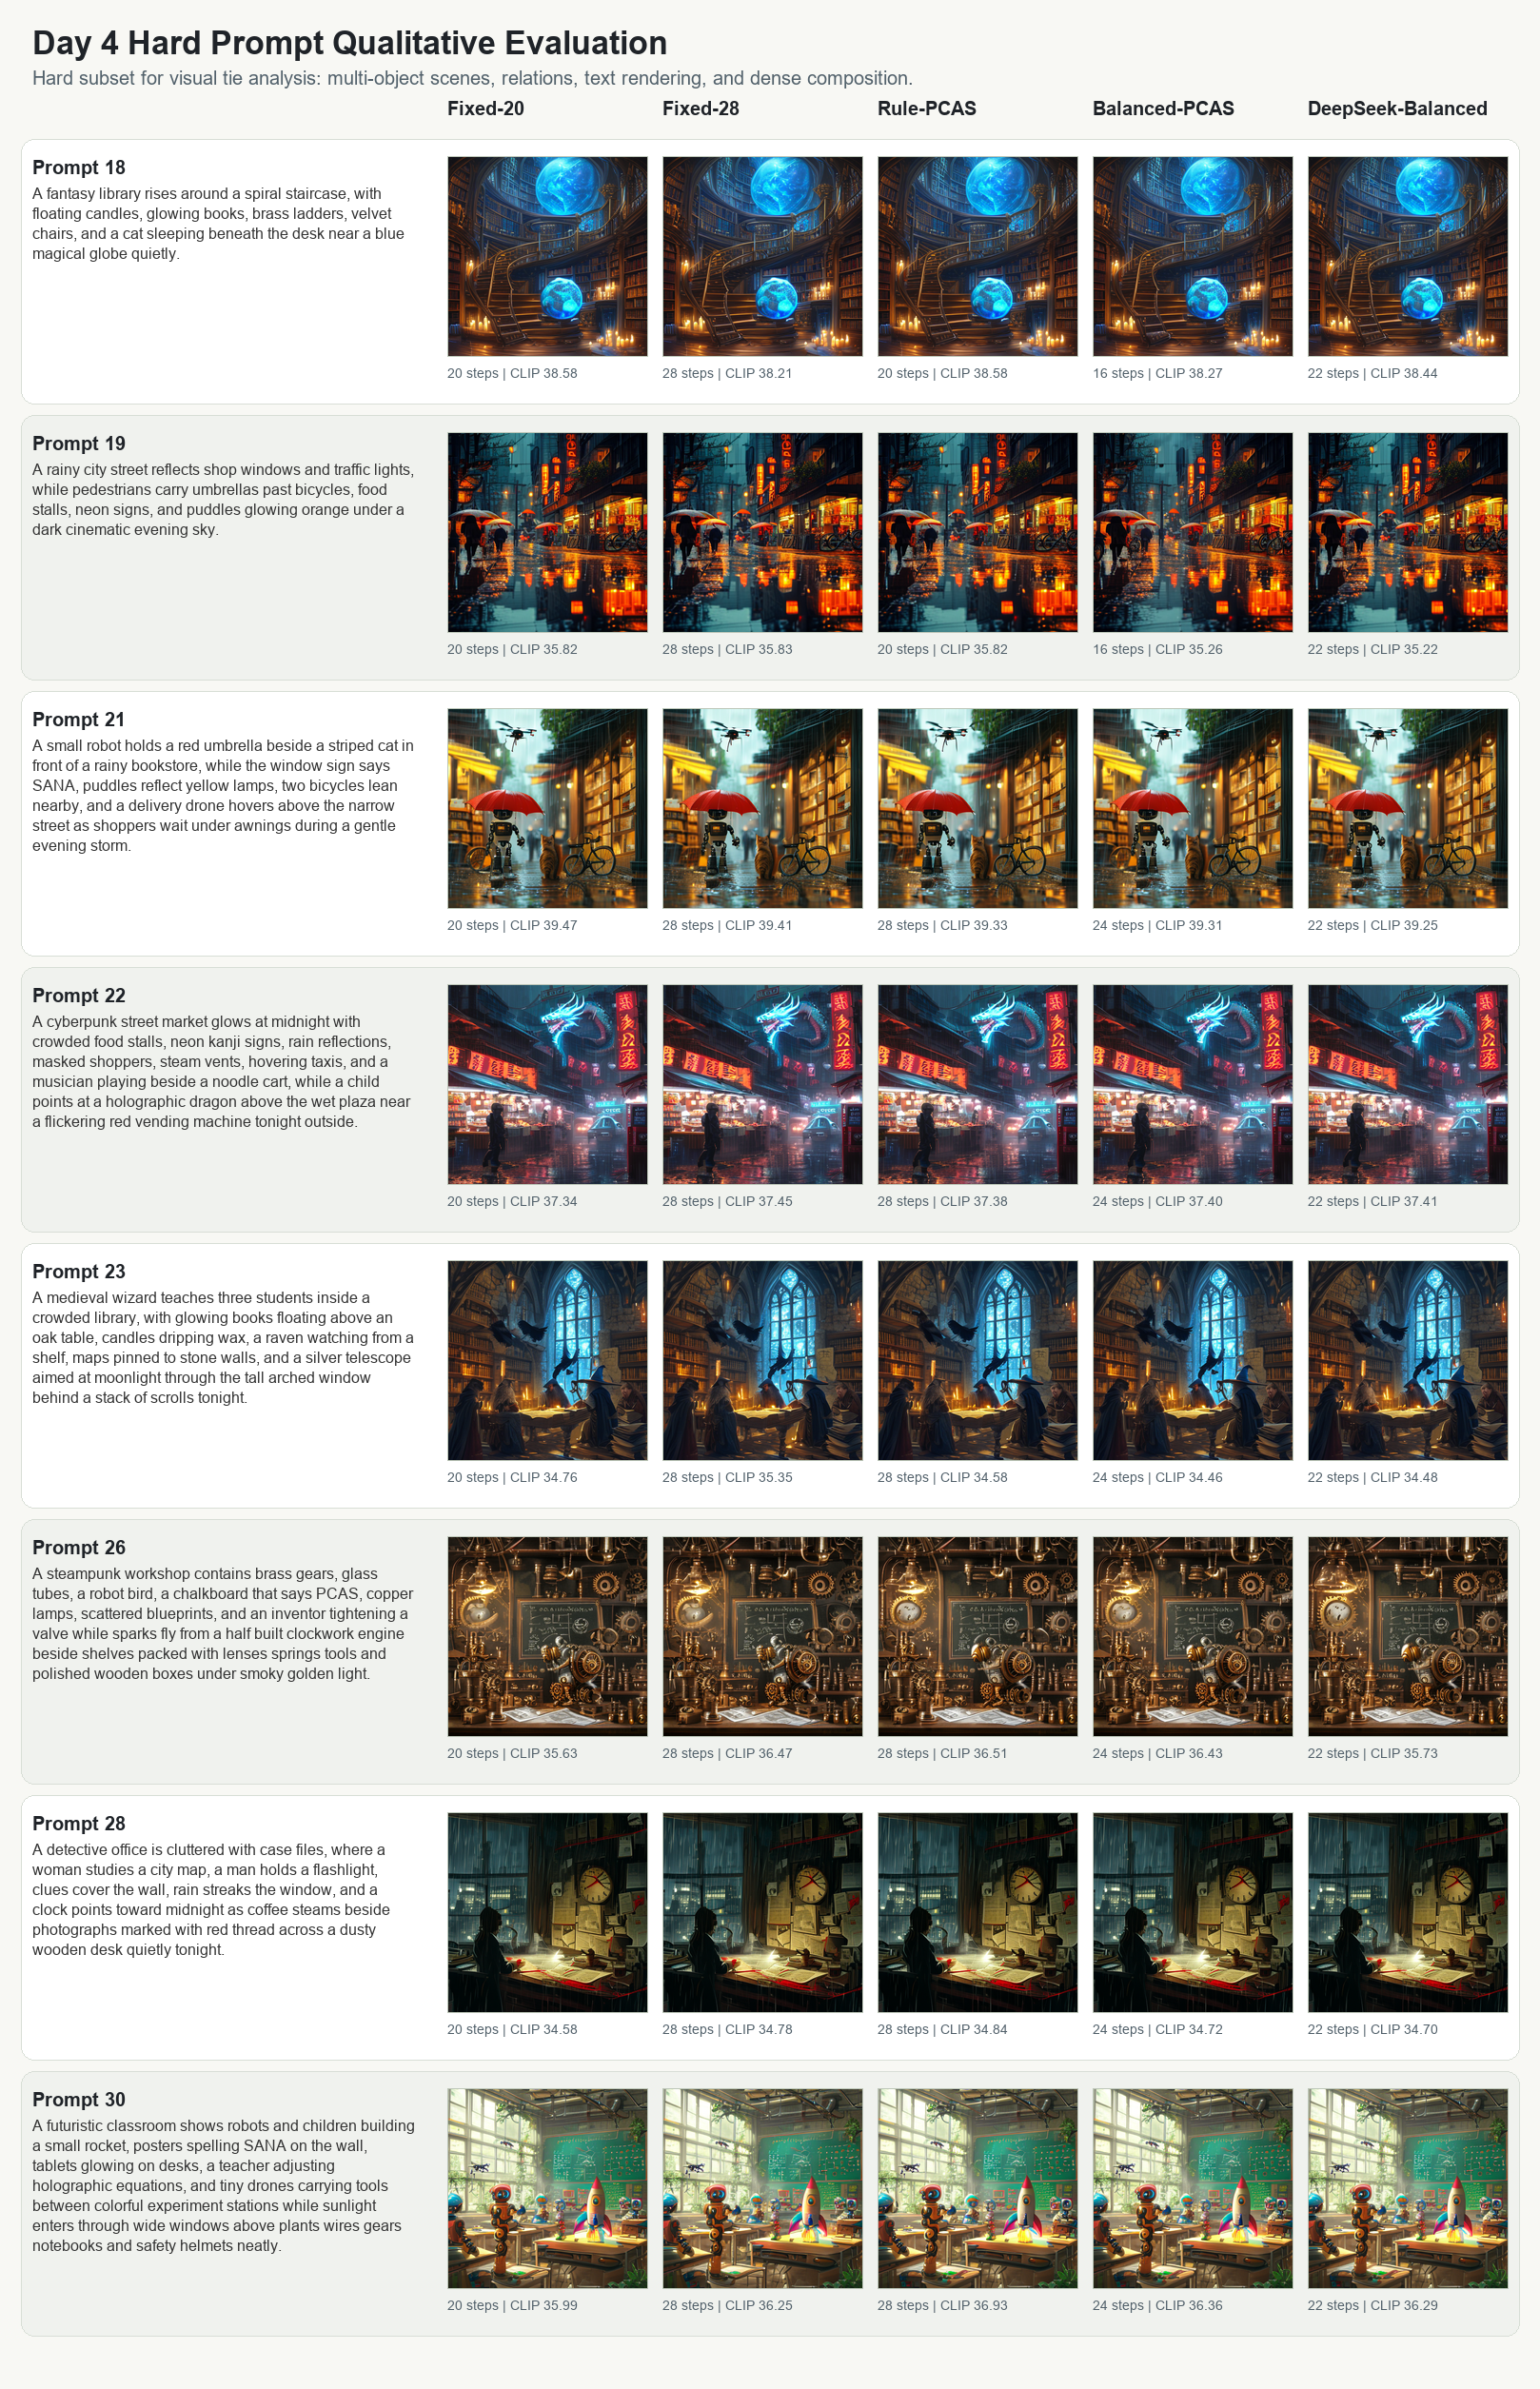
\includegraphics[height=0.82\textheight,keepaspectratio]{day4_hard_prompt_qualitative_grid.png}
  \caption{Hard prompt 子集下不同采样策略的定性对比。多数差异主要体现为局部纹理、光照和小物体细节，而非稳定的语义优劣。}
  \label{fig:hard_grid}
\end{figure}

\cref{tab:hard_prompt} 和 \cref{fig:hard_grid} 显示，Hard subset 上不同方法仍然处在较窄的 \clipscore{} 区间内。视觉差异热图进一步显示，与 Fixed-20 相比，各方法的差异多为局部变化，而不是一致的结构性改进。Balanced-PCAS 在 hard subset 上的平均时间为 0.953s，略快于 Fixed-20 的 0.978s，平均 \clipscore{} 为 36.526，与 Fixed-20 的 36.522 几乎相同。这一结果进一步支持本文结论：PCAS 的贡献是保留视觉和自动对齐水平的同时改善计算分配，而不是稳定提高生成质量。

\subsection{LoRA 个性化实验}

LoRA 扩展实验使用用户提供的黑色头戴式耳机照片训练 SANA-LoRA。原始 LoRA 使用 9 张训练图、rank=8、alpha=8、200 steps；增强版 LoRA 使用 rank=16、alpha=16、500 steps，并使用更明确的 instance prompt；clean-captioned LoRA 筛选 7 张更干净训练图并为每张图添加 sidecar caption。

初始 6 条验证 prompt 显示，LoRA adapter 能够加载并生成有效图像，但 scale=1.0 与 Base 差异较小，scale=2.0 在部分产品照和微距场景中更接近黑色头戴耳机，却未在参考图 CLIP 相似度上稳定超过 Base。为减少遮挡和复杂场景对判断的干扰，本文进一步构造 8 条 subject-focused prompt，要求耳机居中、无遮挡，并明确包含黑色包耳式、椭圆耳罩和厚头梁等属性。

\begin{table}[H]
  \centering
  \caption{Subject-focused LoRA 验证结果}
  \label{tab:lora_subject}
  \begin{tabular}{lrrrr}
    \toprule
    方法 & Ref sim & Ref wins & Subject CLIP & Prompt \clipscore{} \\
    \midrule
    Base & 83.659 & 0/8 & 28.487 & 31.525 \\
    Original LoRA x2 & 83.839 & 4/8 & 29.141 & 32.620 \\
    Enhanced LoRA x1.5 & 81.560 & 2/8 & 30.053 & 34.040 \\
    Enhanced LoRA x2 & 76.666 & 0/8 & 27.874 & 32.855 \\
    Clean-caption x1.25 & 83.281 & 5/8 & 28.982 & 33.084 \\
    Clean-caption x1.5 & 81.778 & 4/8 & 28.646 & 32.752 \\
    Clean-caption x1.75 & 79.343 & 2/8 & 28.401 & 32.887 \\
    \bottomrule
  \end{tabular}
\end{table}

\begin{figure}[H]
  \centering
  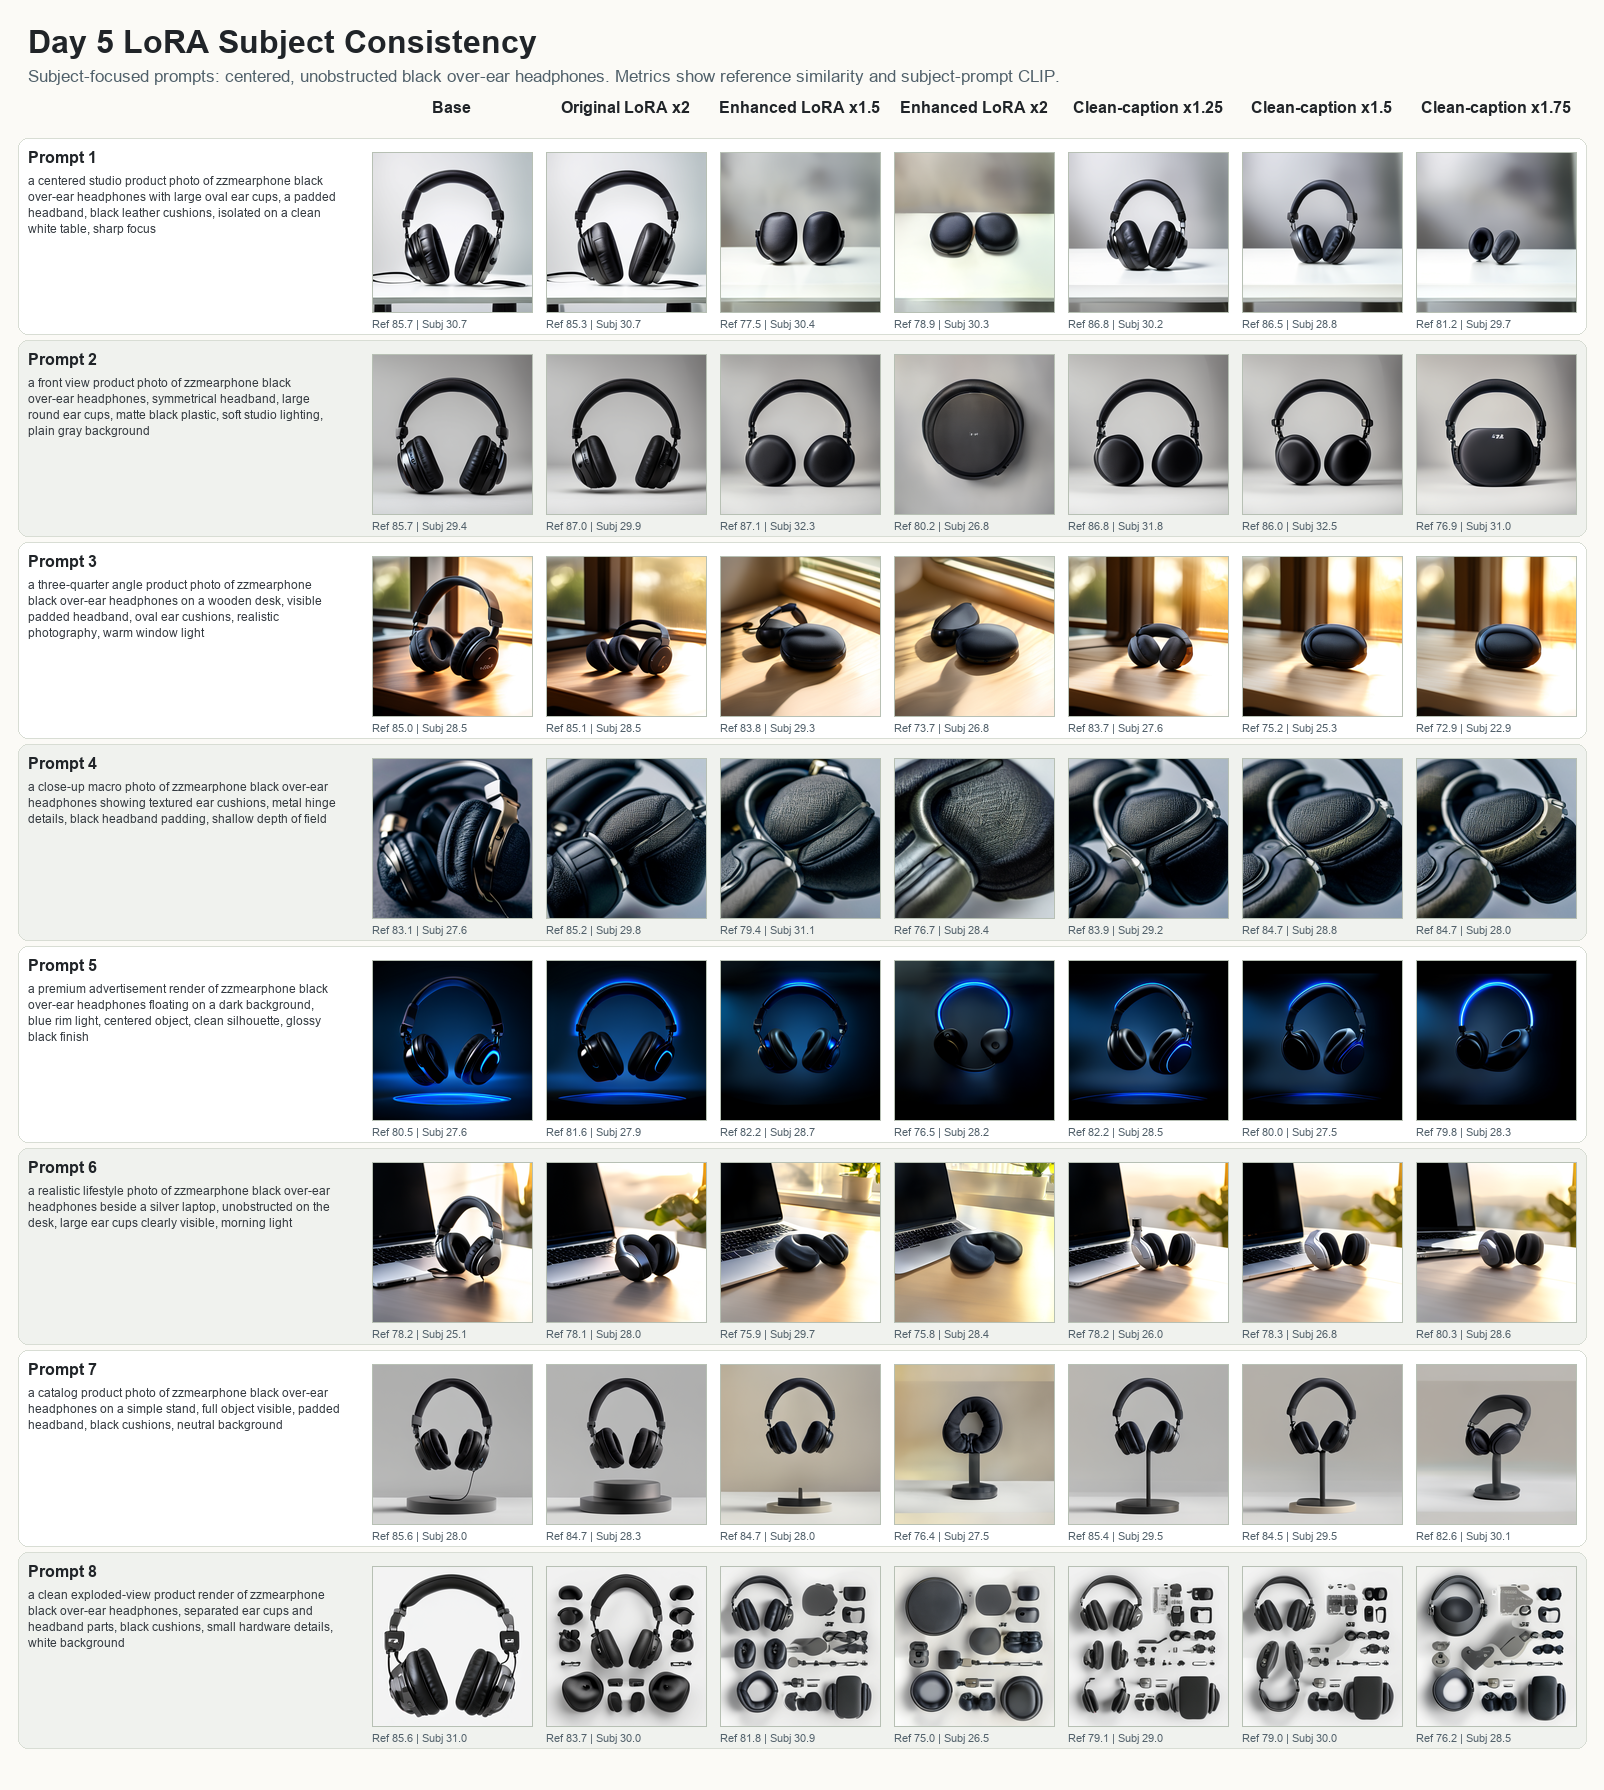
\includegraphics[width=\linewidth,height=0.76\textheight,keepaspectratio]{day5_lora_subject_consistency_grid.png}
  \caption{LoRA 主体一致性验证。Enhanced LoRA x1.5 在主体描述和 prompt 对齐上最强，Clean-caption x1.25 更保守稳定。}
  \label{fig:lora_subject}
\end{figure}

结果显示，Enhanced LoRA x1.5 在 subject-prompt CLIP 和 prompt \clipscore{} 上最佳，说明更明确的 caption、更高 rank 和更长训练确实增强了“黑色头戴式耳机”这一语义绑定。但 Enhanced x2 和 Clean-caption x1.75 都可能出现结构过度简化或形变，说明 adapter scale 并非越高越好。Clean-caption x1.25 虽然不是自动指标最高点，却保持参考相似度接近 Base，并在 5/8 条 prompt 上参考相似度高于 Base，是更保守、更稳定的 clean-data compromise。LoRA 部分因此应作为流程可行性和小样本局限分析，而不是强身份复制结论。

\section{讨论}

\subsection{PCAS 相对于原始 SANA 固定推理的优势}

本文最重要的结论是：\textbf{在不重新训练 SANA 主模型的前提下，PCAS 可以通过 prompt-aware 推理调度显著降低平均推理时间。} 这与 SANA 本身的贡献是互补关系。SANA 通过模型结构设计降低单次高分辨率生成的基础成本，而 PCAS 在已有 SANA pipeline 上进一步减少对所有 prompt 使用同一预算造成的浪费。

相对于直接使用原始 SANA 的 Fixed-20 推理，Balanced-PCAS 的优势主要包括：
\begin{enumerate}
  \item \textbf{平均延迟降低。} Balanced-PCAS 将平均时间从 0.996s 降至 0.751s，获得约 24.6\% 的整体加速。
  \item \textbf{自动对齐指标基本保持。} Balanced-PCAS 的平均 \clipscore{} 为 35.772，与 Fixed-20 的 35.762 基本一致。
  \item \textbf{显存开销不增加。} 所有 PCAS 方法均复用同一 SANA pipeline，平均峰值显存仍约 6.979GB。
  \item \textbf{策略可解释。} 8/16/24 steps 对应简单、中等、复杂 prompt 的预算差异，便于方法说明和工程实现。
  \item \textbf{可扩展。} DeepSeek-Balanced 说明复杂度估计模块可以从词数规则扩展到 LLM 语义标签，未来也可替换为更强的 classifier 或 VQA-based estimator。
\end{enumerate}

因此，PCAS 的优势并不体现为直接提高生成质量上限，而体现为更有效地分配原始 SANA 的固定推理预算。这对真实部署尤其有意义：如果用户请求中存在大量简单产品图、头像、物体或单场景 prompt，固定 20 或 28 steps 会积累可观冗余；PCAS 可以在不牺牲自动对齐指标的前提下减少平均成本。

\subsection{从复杂度估计到预算动作的校准}

本文实验中两个初始结果共同表明，复杂度估计本身并不足以保证自适应推理收益。Rule-PCAS 的直觉是合理的：短 prompt 可以使用更少 steps，长 prompt 可以保留更多预算；但如果 policy 没有显式控制平均预算，短 prompt 的节省会被长 prompt 的 28 steps 抵消。因此，prompt-aware 并不自动等价于 faster；只有引入预算约束后，自适应策略才会真正带来整体加速。

DeepSeek-PCAS 的结果进一步强调了这一点。LLM 语义复杂度判断倾向于谨慎，尤其面对包含多个对象、风格和关系的 prompt 时更容易输出 high。如果 policy 将 high 直接映射到 28 steps，LLM 复杂度估计会把系统推向更慢的质量保守模式。DeepSeek-Balanced 说明，复杂度标签与采样动作应该分离：标签负责描述输入难度，policy 负责在给定延迟预算下选择动作。未来更完整的系统可以把 policy 写成显式优化问题，例如在满足最大平均延迟的约束下最大化质量代理指标。

\subsection{Calibrated-PCAS 的机制与证据}

Balanced-PCAS 证明 8/16/24 的预算约束能在平均意义上提高效率，但它仍是人工策略，无法解释为什么某条 50-word prompt 可以只用 8 steps，也无法保证每条 prompt 都接近 Fixed-20 的质量参考。Calibrated-PCAS 将这一局限转化为逐 prompt 的约束优化问题：先在多档 steps 下实际生成图像，再用 \clipscore{} 相对 Fixed-20 的容忍阈值定义 minimal sufficient steps，最后训练轻量 decision tree 近似 oracle policy。

这一实验带来三点结论。第一，在当前 benchmark 中，最小充分 steps 明显低于固定 20 steps：18/30 条 prompt 的标签为 8 steps，4 条为 12 steps，6 条为 16 steps，只有 2 条仍需要 20 steps。第二，数据校准 policy 比手工 policy 更贴近逐 prompt 约束：Balanced-PCAS 和 DeepSeek-Balanced 的 Fixed-20 约束满足率均为 73.3\%，而 rule-feature 与 LLM-feature Calibrated-PCAS 均达到 96.7\%。第三，LLM features 并不自动显著优于 rule features；在 30 条小样本下，两者约束满足率相同，说明语义特征需要更多样本和更稳健的校准才能稳定超过可复现规则特征。

因此，本文的核心结论可以概括为：\textbf{Balanced-PCAS 是当前最稳健的效率主结果，Calibrated-PCAS 则把 PCAS 从经验规则推进到数据校准的最小预算预测框架。} 前者支撑主要速度收益，后者为更大规模 prompt 分布上的学习式推理调度提供方法基础。

\subsection{质量结论的边界}

本文没有声称 PCAS 显著提升图像质量，这是一个重要且必要的证据边界。质量评价结果表明，各方法 \clipscore{} 差异很小；Hard prompt 定性图也显示，多数差异只是局部纹理、光照或小物体细节变化。相较于将小幅指标波动解释为质量提升，更稳健的表述是：PCAS 在保持质量近似不变的条件下改善效率。

这并不削弱 PCAS 的价值。相反，如果 Balanced-PCAS 在减少约四分之一平均时间后仍保持接近 Fixed-20 的 \clipscore{}，它已经达成了效率策略的核心目标。工程上，质量保持本身就是重要结果：当一个方法能显著降低延迟且不引入明显质量下降时，就具备实际意义。未来若要证明质量提升，需要更大规模样本、人工偏好评分、VQA-based 关系检测、对象计数准确性、文字渲染准确率和审美模型等更多证据。

\subsection{Guidance scale 的启示}

Guidance scale 消融显示，中等 guidance 区间相对鲁棒，1.5 明显较弱，而 8.5 只在自动 \clipscore{} 上表现出轻微偏好。该结果提示，guidance scale 并非简单“越高越好”。高 guidance 可能强化文本对齐，也可能带来构图僵硬、过强对比、过饱和或局部细节取舍。本文最终没有将 guidance scale 作为主线优化点，而是在 Balanced-PCAS 中进行温和调整，这是较稳妥的选择。

更进一步，guidance scale 也可以纳入未来 PCAS 的多目标调度：复杂 prompt 或带文字 prompt 可以略提高 guidance，简单物体 prompt 可以使用较低 guidance 以减少过度约束。但这种策略需要更多定性检查和自动指标支持，不能仅凭当前小规模消融得出强结论。

\subsection{LoRA 个性化实验的意义与限制}

LoRA 扩展实验说明，在同一硬件条件下复现 SANA DreamBooth LoRA 是可行的，但小样本主体一致性并不稳定。原始 LoRA x2 与训练图参考中心最接近，但提升很小；Enhanced LoRA x1.5 在主体描述和 prompt 对齐上最好，但参考图相似度下降；Clean-caption x1.25 更保守，视觉上也较少出现强 scale 导致的结构坍塌。

这说明个性化生成的难点不仅在于能否训练 LoRA，还包括训练图是否覆盖足够视角、caption 是否精确、adapter scale 是否合适，以及评价指标是否能真正衡量产品身份。CLIP 图像相似度只能粗略判断是否像“耳机”，不能精确判断是否复现某一副耳机的耳罩形状、折叠结构或材质细节。因此，本文将 LoRA 作为探索性增强，而不是主线强结果。

\subsection{局限性}

本文仍存在若干局限：
\begin{enumerate}
  \item \textbf{Benchmark 规模有限。} 当前只有 30 条受控 prompt，虽然便于分析，但不足以代表真实用户 prompt 分布。
  \item \textbf{复杂度特征仍需更多验证。} 本文已经从词数分组扩展到 rule features 与 DeepSeek JSON features，但 decision tree 仍只在 30 条 prompt 上校准，尚未证明在真实 prompt 分布上稳定泛化。
  \item \textbf{质量评价以 CLIPScore 为主。} CLIPScore 对局部结构、对象关系和审美质量不敏感，缺少人工评分和 VQA-based 指标。
  \item \textbf{未系统测试 adaptive resolution。} 原始大纲中提到 steps、guidance 与 resolution 的联合自适应，但本文实际主线固定 512$\times$512。
  \item \textbf{LLM 特征的收益尚不稳定。} DeepSeek JSON features 已接入 Calibrated-PCAS，但当前结果与 rule features 接近；不同 LLM、不同 prompt 分布和 API 成本对策略的影响尚未评估。
  \item \textbf{LoRA 数据量较少。} 9 张训练图不足以支撑稳定产品身份复制，当前只能说明流程可行和局限存在。
  \item \textbf{硬件与模型规模受限。} 本文未全面测试 SANA 1.6B、更高分辨率或其他高效 backbone 下的迁移效果。
\end{enumerate}

\subsection{未来工作}

未来可以从四个方向扩展。第一，扩大 prompt benchmark，将真实用户 prompt、中文 prompt、带文字生成 prompt 和更复杂多主体场景纳入评估，并重新训练 Calibrated-PCAS predictor。第二，引入更强质量指标，包括人工偏好评分、ImageReward、PickScore、VQA-based object/relationship metrics 和 OCR-based text rendering accuracy，使 minimal sufficient steps 不只依赖 \clipscore{}。第三，将 PCAS 从 steps/guidance 扩展到 adaptive resolution、adaptive solver order 或 early stopping，从而形成更完整的多维预算调度。第四，针对 LoRA 个性化补充更干净、多角度、高一致性的产品图，并结合 identity-aware 指标进行评价。

\section{结论}

本文围绕高效文生图模型 SANA 展开，完成了 SANA-0.6B diffusers 推理复现、受控 prompt benchmark 构建、固定步数 baseline 对比、Prompt-Complexity Adaptive Sampling 设计与系统评估。实验结果表明，即使 SANA 本身已经是高效 backbone，固定采样参数仍然会在不同 prompt 之间造成计算预算分配不均。PCAS 通过 prompt-aware 推理调度，在不修改主模型参数的前提下改善了这一问题。

具体而言，原始 Rule-PCAS 展示了根据 prompt 长度重新分配 steps 的可行性，但整体加速有限；Balanced-PCAS 通过 8/16/24 steps 的预算约束策略，将平均推理时间从 Fixed-20 的 0.996s 降至 0.751s，实现约 24.6\% 加速，同时保持 \clipscore{} 基本不变。DeepSeek-PCAS 证明 LLM 语义复杂度判断可以用于调度，但原始策略过于保守；DeepSeek-Balanced 通过更温和的 8/16/22 steps 策略，将平均时间降至 0.844s，相比 Fixed-20 快约 15.3\%。

进一步地，Calibrated-PCAS 将复杂度估计、预算动作和质量约束放入同一 calibration framework。通过 $\{8,12,16,20,24,28\}$ calibration grid，本文得到逐 prompt 的 minimal sufficient steps 标签：18 条 prompt 只需 8 steps，4 条需要 12 steps，6 条需要 16 steps，2 条需要 20 steps。在该 calibration set 上，rule-feature 和 LLM-feature Calibrated-PCAS 都以约 10--11 个平均 steps 达到 96.7\% 的 Fixed-20 约束满足率，明显高于 Balanced-PCAS 和 DeepSeek-Balanced 的 73.3\%。这说明 PCAS 不必停留在手工分组策略，而可以被表述为可解释的数据校准推理预算预测框架。

质量分析显示，各方法之间的 \clipscore{} 差异较小，hard prompt 定性结果也未支持显著质量上限提升。因此，本文将 PCAS 定位为一种保持自动文本对齐指标并改善效率--质量权衡的推理调度策略，而不是显著提升图像质量的方法。最后，SANA-LoRA DreamBooth 扩展实验说明小样本个性化流程可行，但主体一致性仍受数据、caption 和 adapter scale 明显影响。整体而言，本文形成了一个可复现的 SANA 推理评估流程，并为更大规模 prompt 分布、更丰富质量指标和 adaptive resolution 研究提供了基础。

\clearpage
\begin{thebibliography}{99}
\bibitem{xie2024sana}
Xie, E. et al. \textit{SANA: Efficient High-Resolution Image Synthesis with Linear Diffusion Transformers}. arXiv:2410.10629, 2024.

\bibitem{nvlabs_sana}
NVlabs. \textit{Sana official repository}. \url{https://github.com/NVlabs/Sana}.

\bibitem{xie2025sana15}
Xie, E. et al. \textit{SANA 1.5: Efficient Scaling of Training-Time and Inference-Time Compute in Linear Diffusion Transformer}. arXiv:2501.18427, 2025.

\bibitem{ho2020ddpm}
Ho, J., Jain, A. and Abbeel, P. Denoising Diffusion Probabilistic Models. \textit{NeurIPS}, 2020.

\bibitem{rombach2022ldm}
Rombach, R. et al. High-Resolution Image Synthesis with Latent Diffusion Models. \textit{CVPR}, 2022.

\bibitem{peebles2023dit}
Peebles, W. and Xie, S. Scalable Diffusion Models with Transformers. \textit{ICCV}, 2023.

\bibitem{radford2021clip}
Radford, A. et al. Learning Transferable Visual Models From Natural Language Supervision. \textit{ICML}, 2021.

\bibitem{hessel2021clipscore}
Hessel, J. et al. CLIPScore: A Reference-free Evaluation Metric for Image Captioning. \textit{EMNLP}, 2021.

\bibitem{hu2022lora}
Hu, E. J. et al. LoRA: Low-Rank Adaptation of Large Language Models. \textit{ICLR}, 2022.

\bibitem{ruiz2023dreambooth}
Ruiz, N. et al. DreamBooth: Fine Tuning Text-to-Image Diffusion Models for Subject-Driven Generation. \textit{CVPR}, 2023.
\end{thebibliography}

\appendix
\section{补充图表}

\subsection{固定步数生成结果网格}

\begin{figure}[H]
  \centering
  \includegraphics[height=0.66\textheight,keepaspectratio]{day2_baseline_grid_10_words_full_prompts.png}
  \caption{10-word prompts 下 Fixed-10、Fixed-20 与 Fixed-28 的生成结果对比。}
  \label{fig:appendix_day2_10}
\end{figure}

\begin{figure}[H]
  \centering
  \includegraphics[height=0.76\textheight,keepaspectratio]{day2_baseline_grid_30_words_full_prompts.png}
  \caption{30-word prompts 下 Fixed-10、Fixed-20 与 Fixed-28 的生成结果对比。}
  \label{fig:appendix_day2_30}
\end{figure}

\begin{figure}[H]
  \centering
  \includegraphics[height=0.76\textheight,keepaspectratio]{day2_baseline_grid_50_words_full_prompts.png}
  \caption{50-word prompts 下 Fixed-10、Fixed-20 与 Fixed-28 的生成结果对比。}
  \label{fig:appendix_day2_50}
\end{figure}

\subsection{原始 PCAS 与 DeepSeek-PCAS 补充图}

\begin{figure}[H]
  \centering
  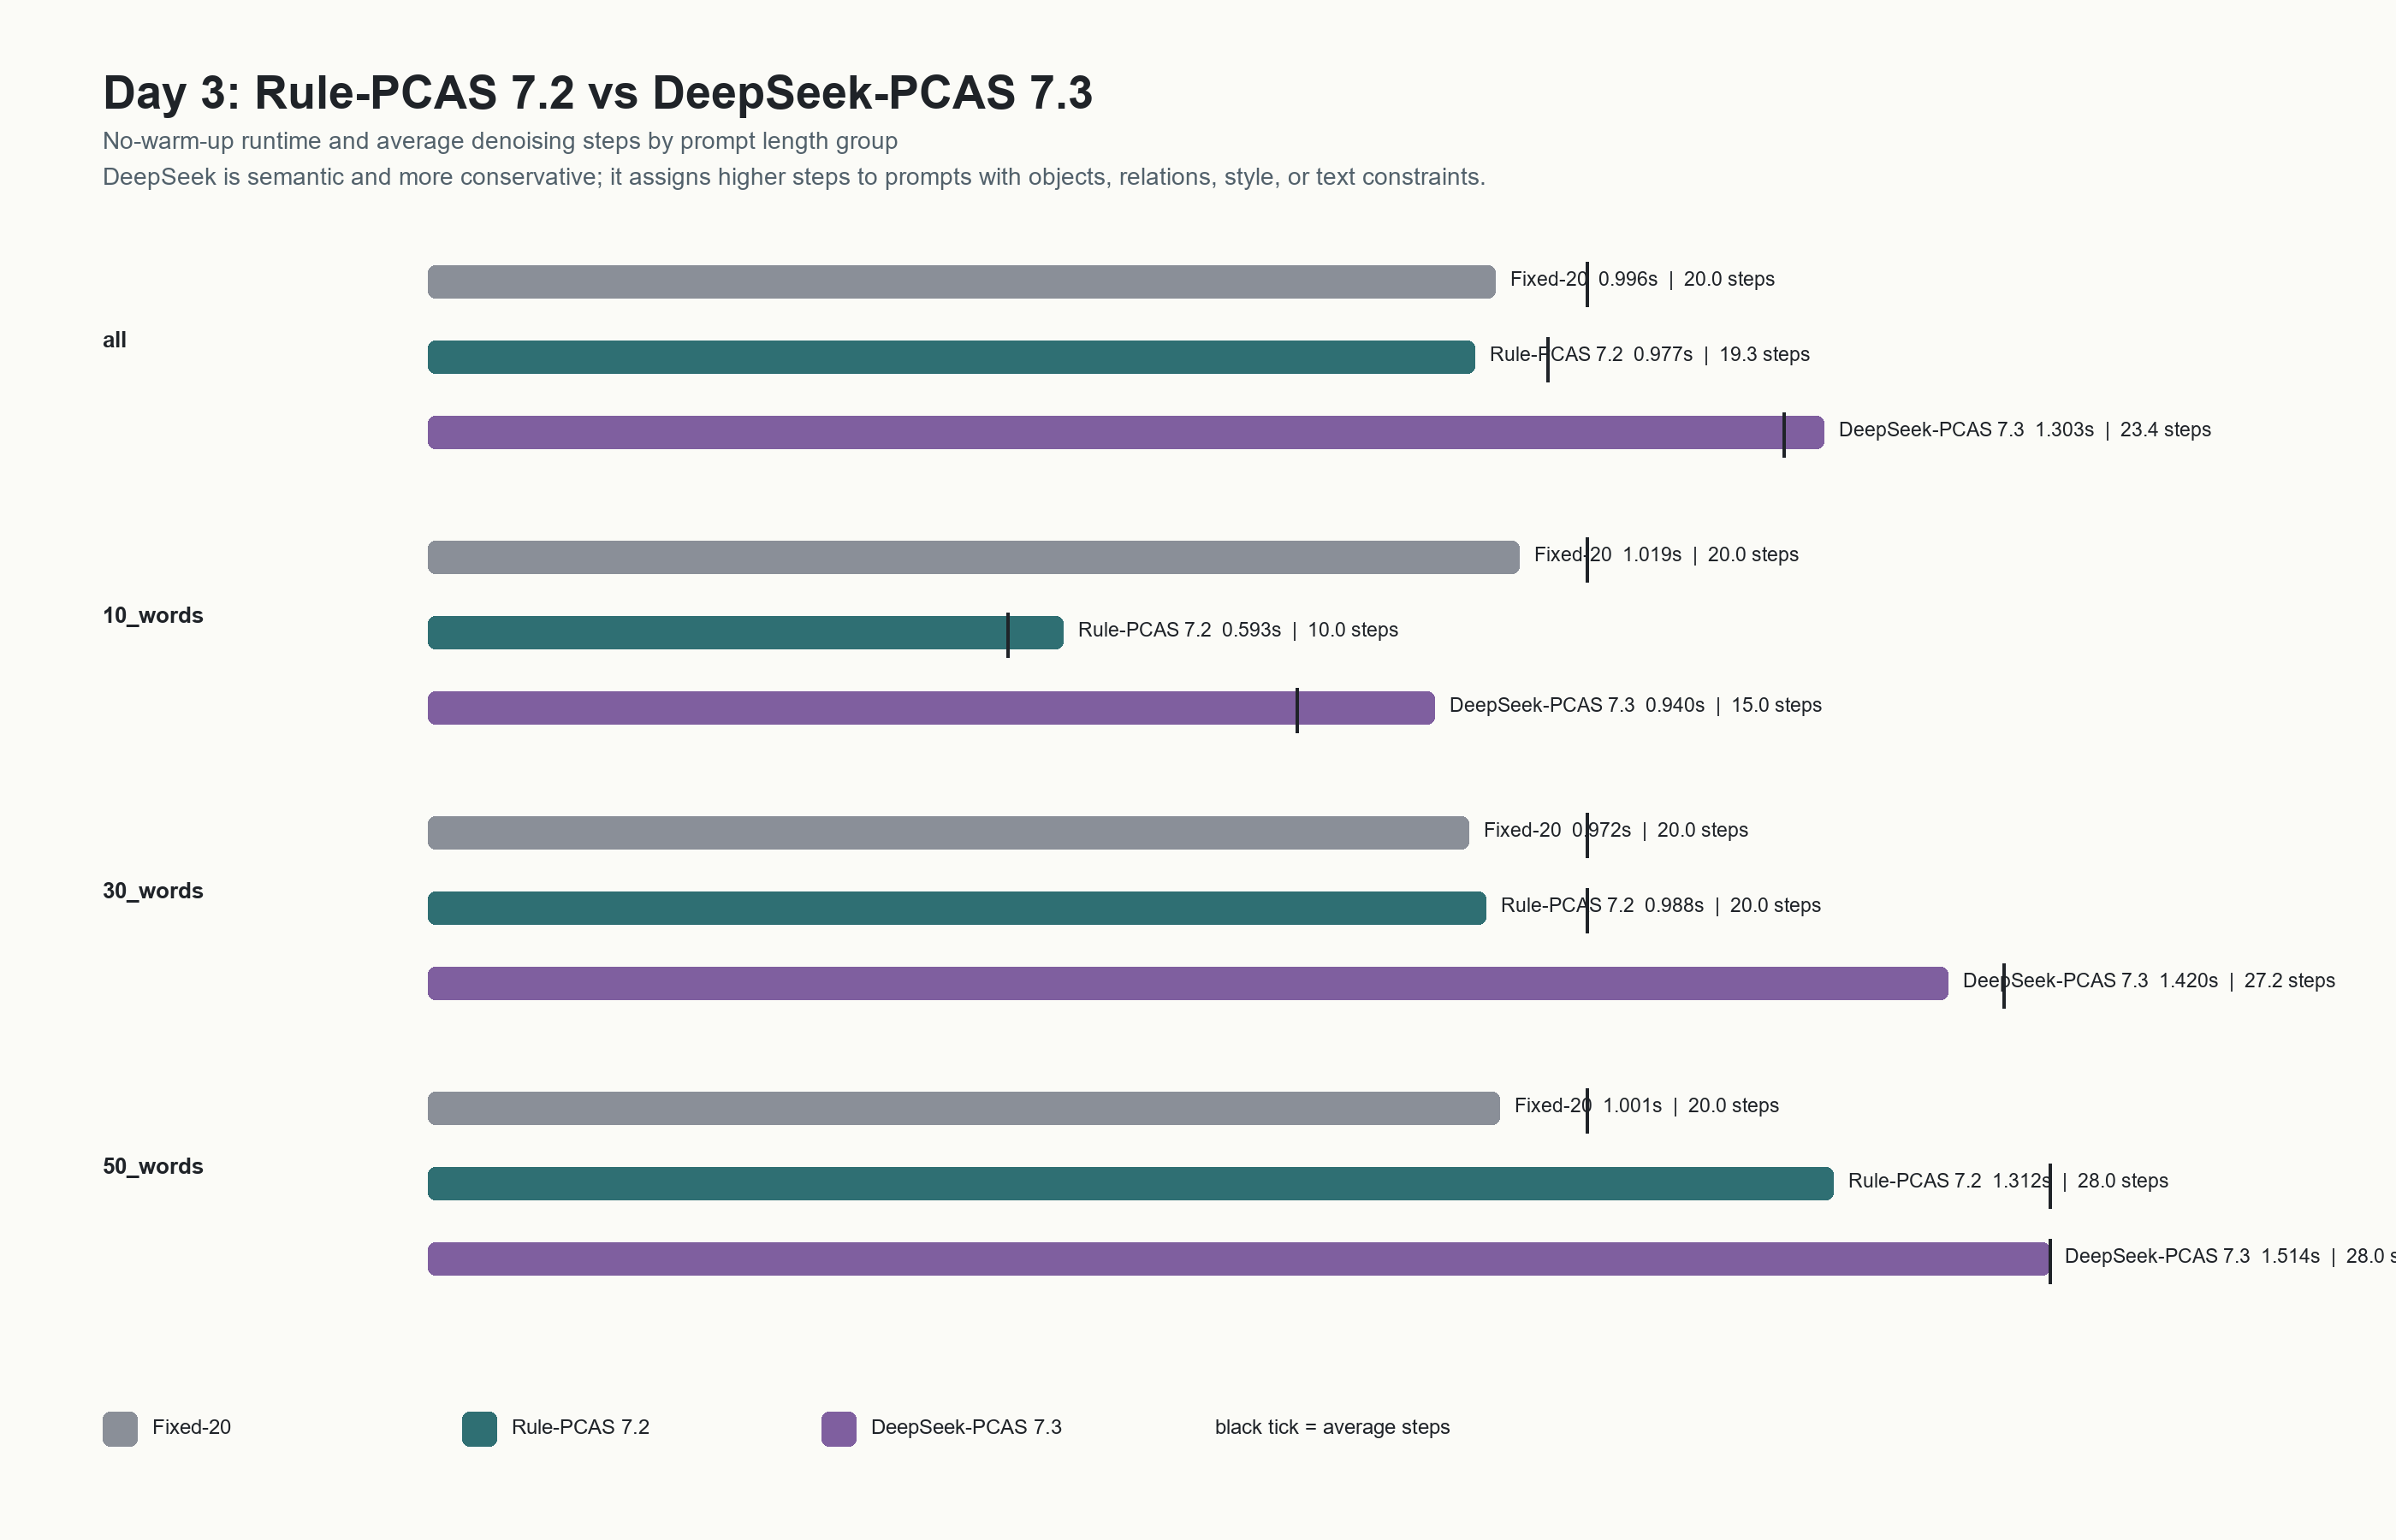
\includegraphics[width=0.86\linewidth]{day3_7_2_vs_7_3_time_steps_chart.png}
  \caption{Rule-PCAS 7.2 与 DeepSeek-PCAS 7.3 的采样步数和时间对比。}
  \label{fig:appendix_rule_deepseek}
\end{figure}

\begin{figure}[H]
  \centering
  \includegraphics[height=0.76\textheight,keepaspectratio]{day3_pcas_vs_fixed20_full_prompts.png}
  \caption{Rule-PCAS 与 Fixed-20 的完整 prompt 对照图。}
  \label{fig:appendix_pcas_full}
\end{figure}

\begin{figure}[H]
  \centering
  \includegraphics[height=0.76\textheight,keepaspectratio]{day3_7_2_vs_7_3_full_prompts.png}
  \caption{Rule-PCAS 与 DeepSeek-PCAS 的完整 prompt 对照图。}
  \label{fig:appendix_deepseek_full}
\end{figure}

\subsection{Guidance 与 hard prompt 补充图}

\begin{figure}[H]
  \centering
  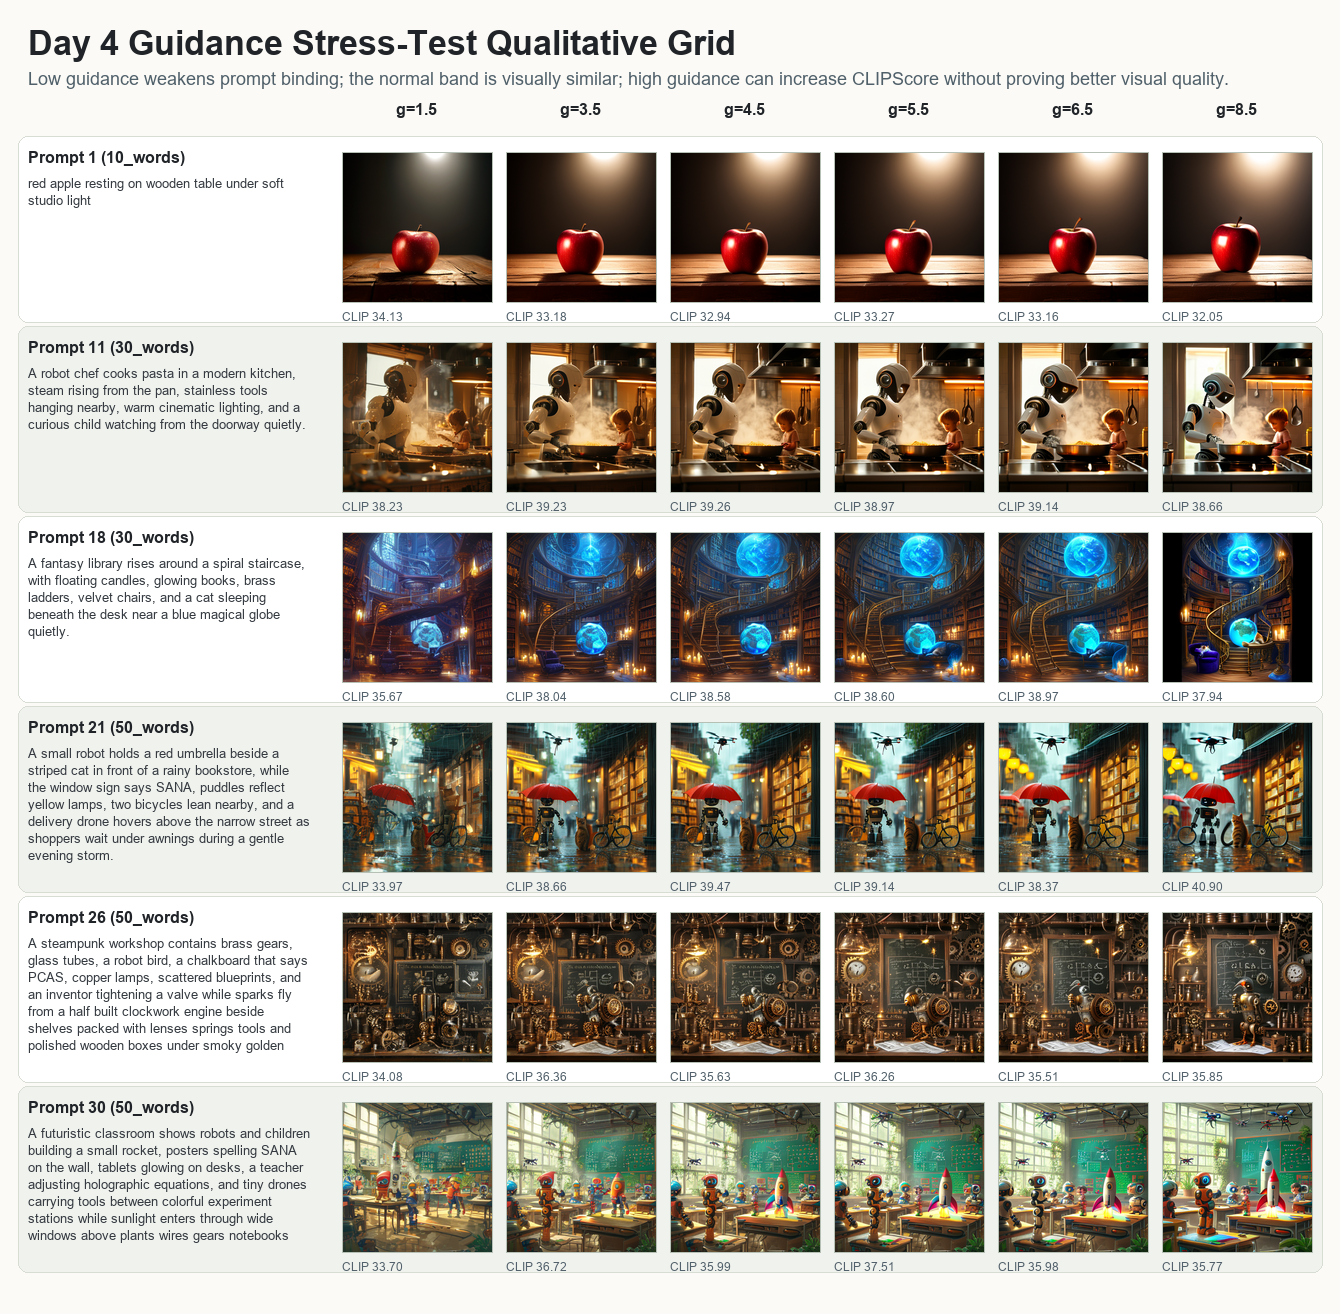
\includegraphics[width=\linewidth]{day4_guidance_stress_qualitative_grid.png}
  \caption{Guidance scale stress-test 定性图。低 guidance 明显削弱文本对齐，高 guidance 需要结合视觉检查。}
  \label{fig:appendix_guidance_stress}
\end{figure}

\begin{figure}[H]
  \centering
  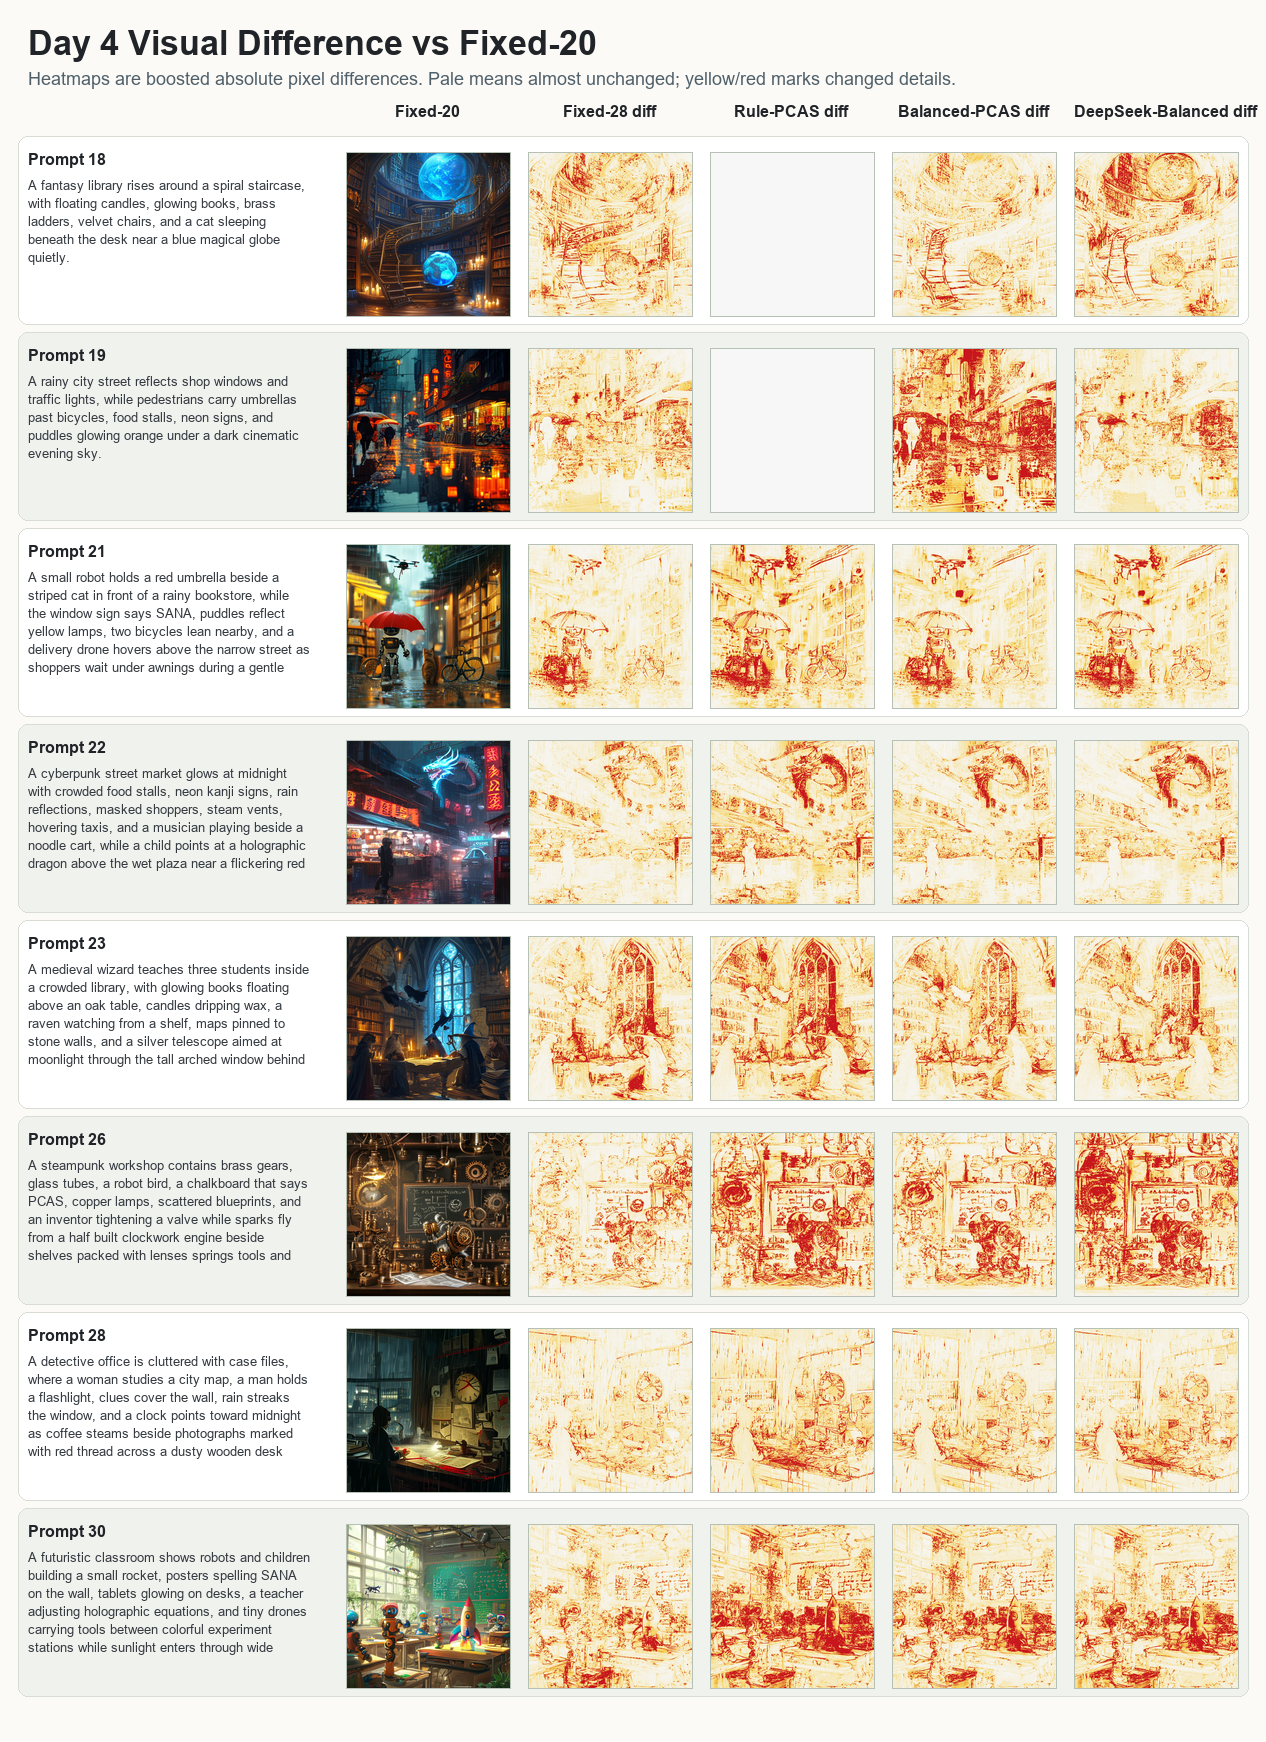
\includegraphics[width=\linewidth]{day4_hard_prompt_difference_heatmap_vs_fixed20.png}
  \caption{Hard prompt 子集中各方法相对 Fixed-20 的视觉差异热图。}
  \label{fig:appendix_diff_heatmap}
\end{figure}

\subsection{LoRA 个性化补充图}

\begin{figure}[H]
  \centering
  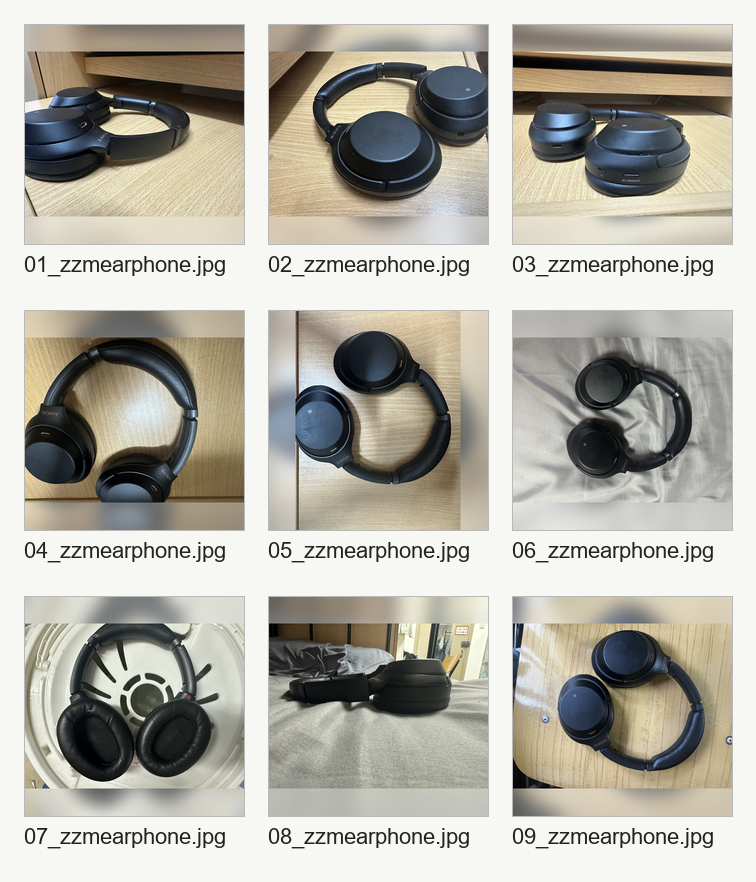
\includegraphics[width=0.88\linewidth]{day5_lora_training_images_contact_sheet.png}
  \caption{LoRA 训练图 contact sheet。数据量较少且视角复杂，是主体一致性不稳定的重要原因。}
  \label{fig:appendix_lora_train}
\end{figure}

\begin{figure}[H]
  \centering
  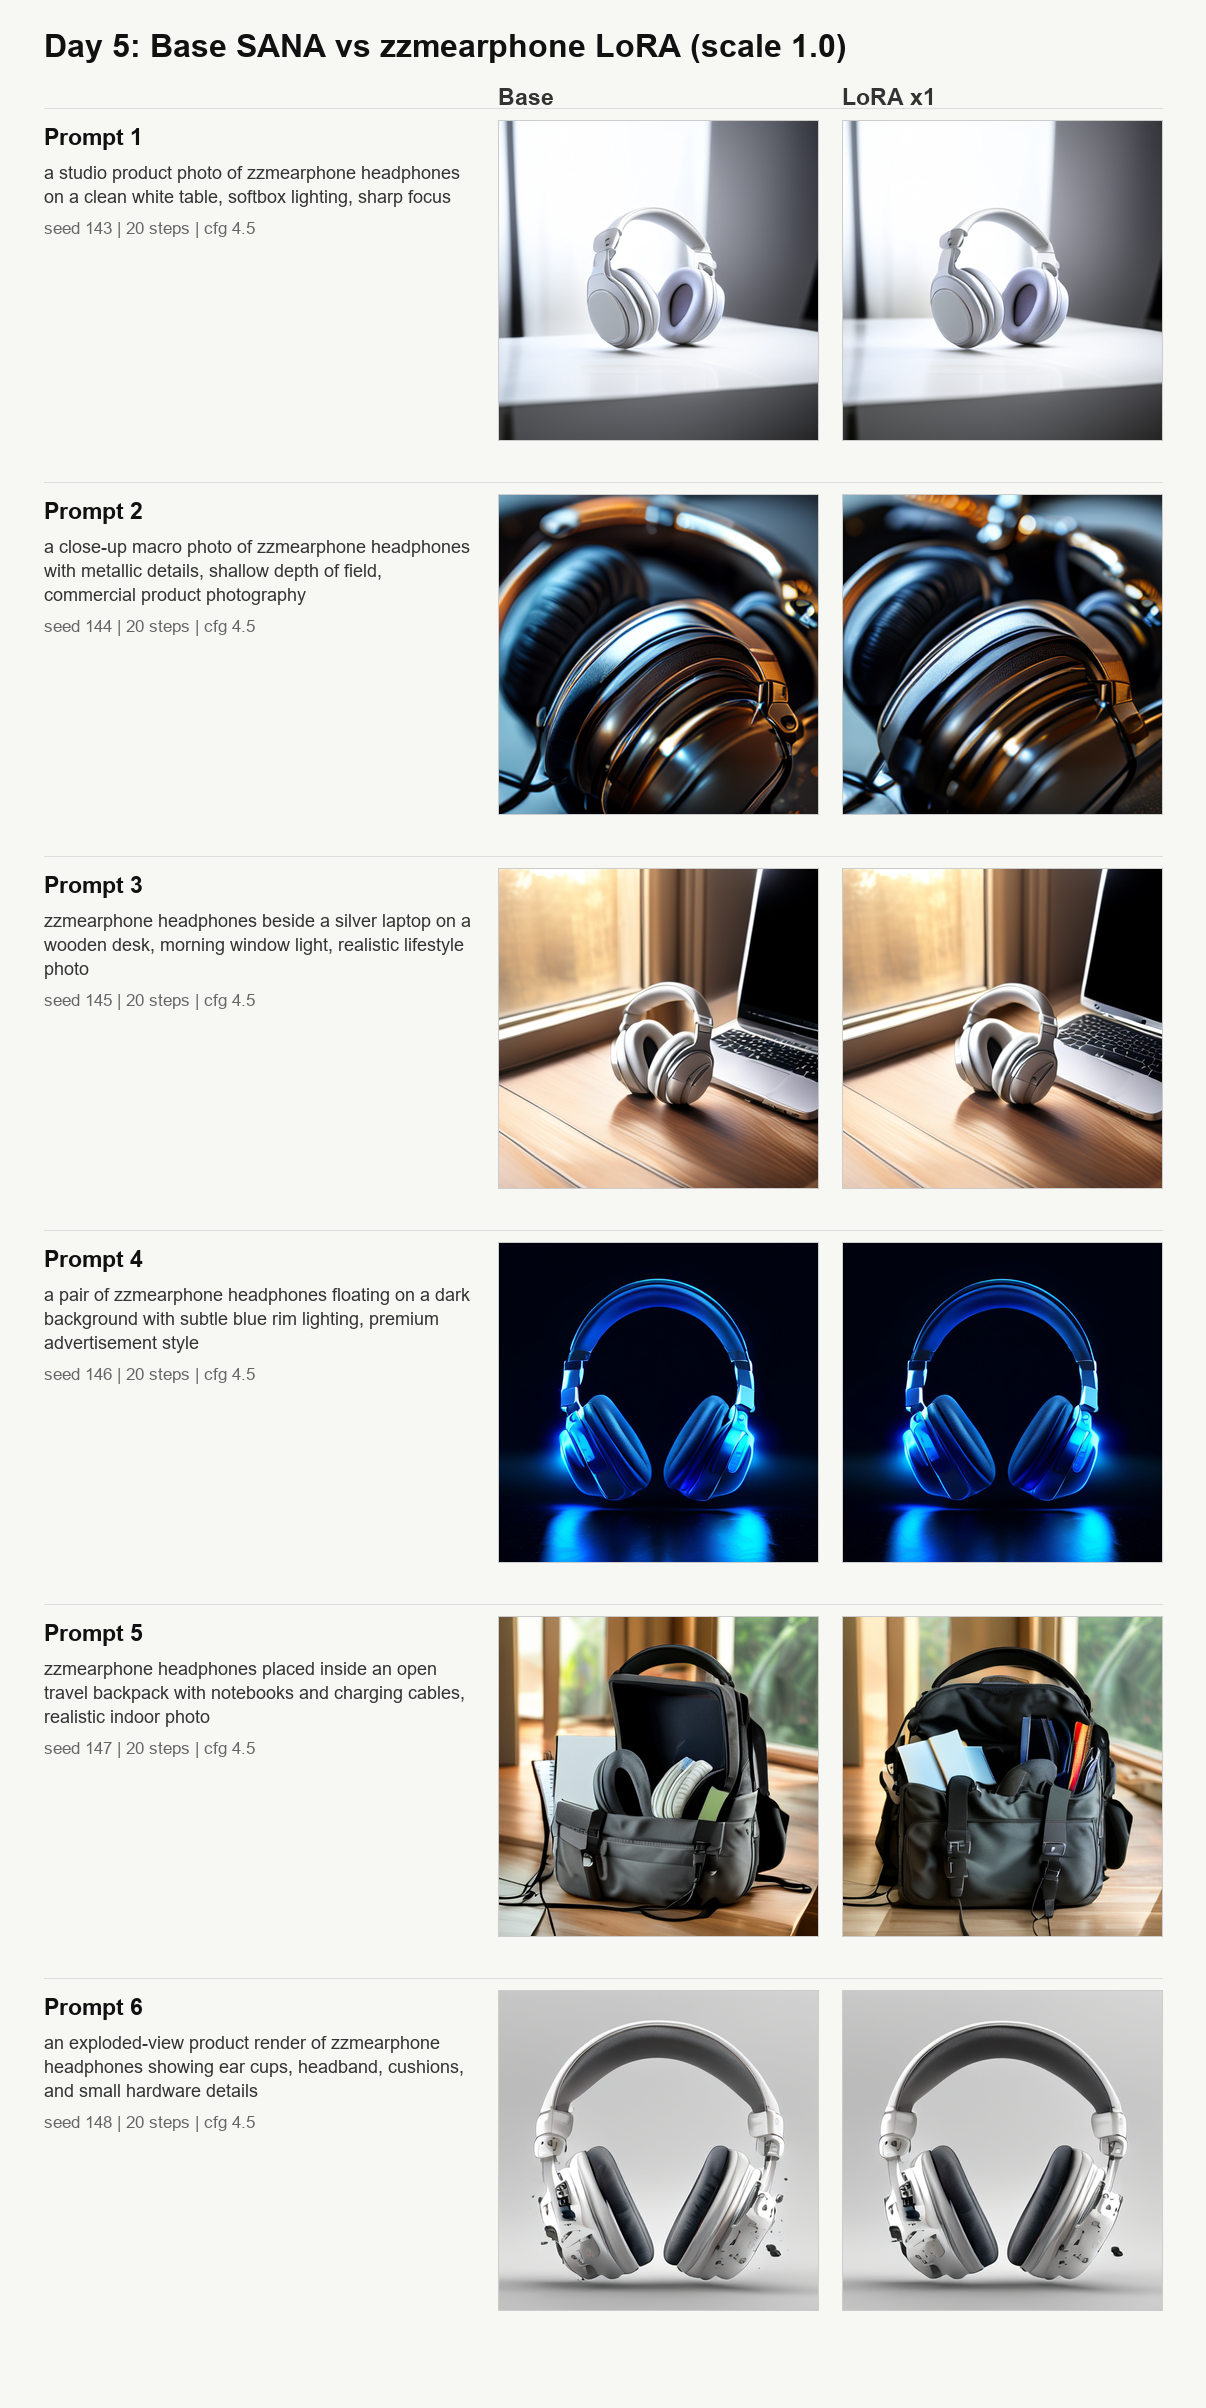
\includegraphics[width=\linewidth]{day5_lora_base_vs_lora_scale1_grid.png}
  \caption{Base SANA 与 LoRA scale=1.0 的验证对比。}
  \label{fig:appendix_lora_scale1}
\end{figure}

\begin{figure}[H]
  \centering
  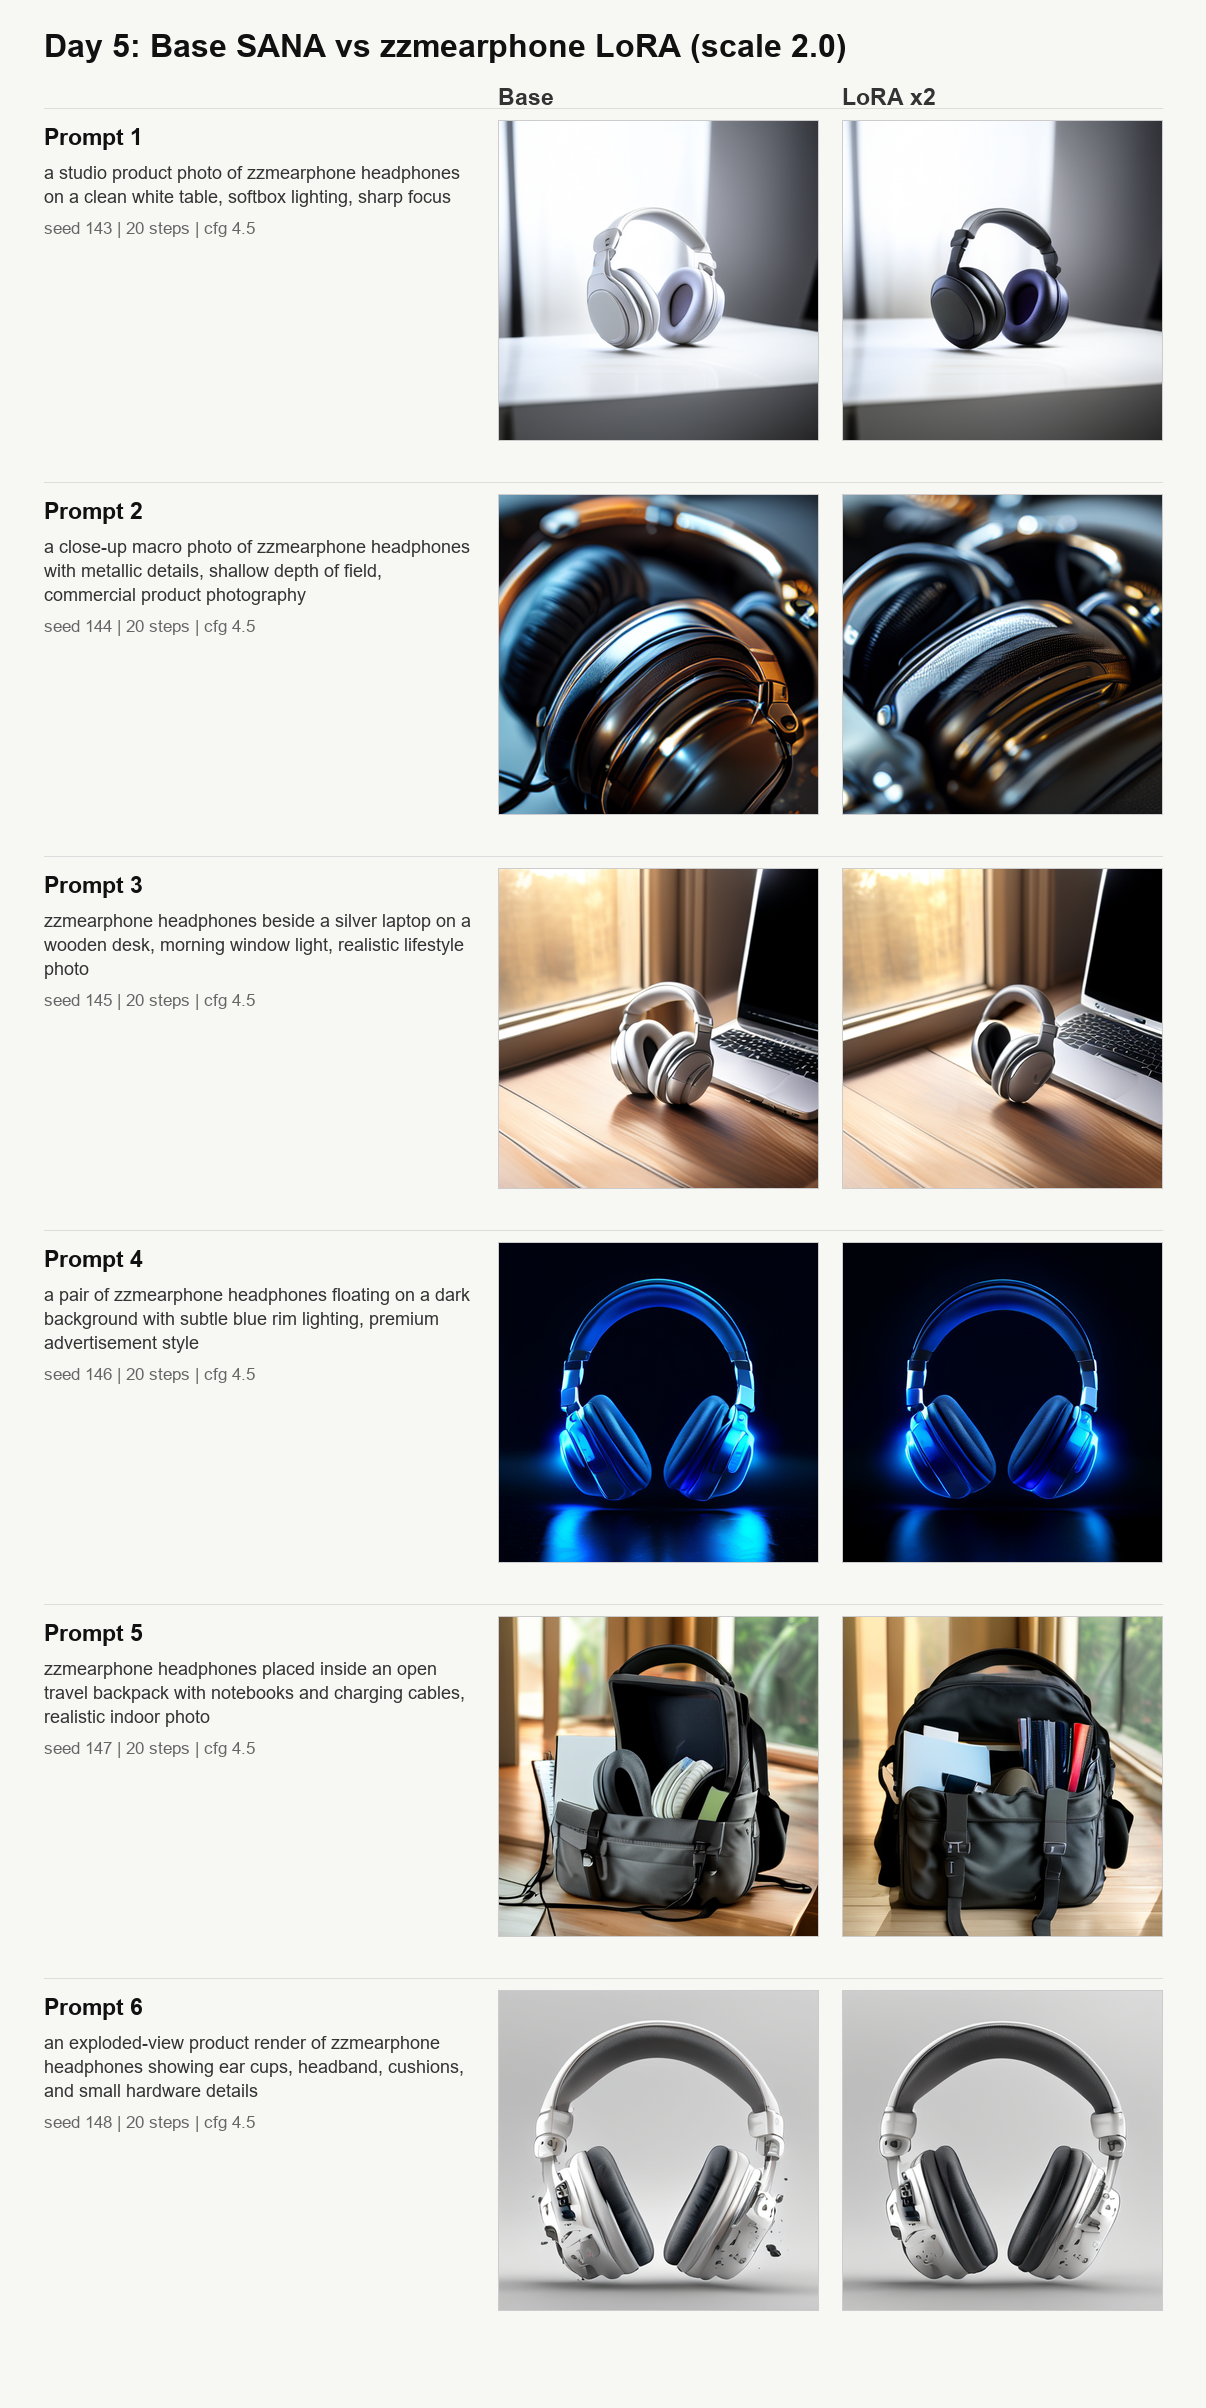
\includegraphics[width=\linewidth]{day5_lora_base_vs_lora_scale2_grid.png}
  \caption{Base SANA 与 LoRA scale=2.0 的验证对比。}
  \label{fig:appendix_lora_scale2}
\end{figure}

\begin{figure}[H]
  \centering
  \begin{subfigure}{0.48\linewidth}
    \centering
    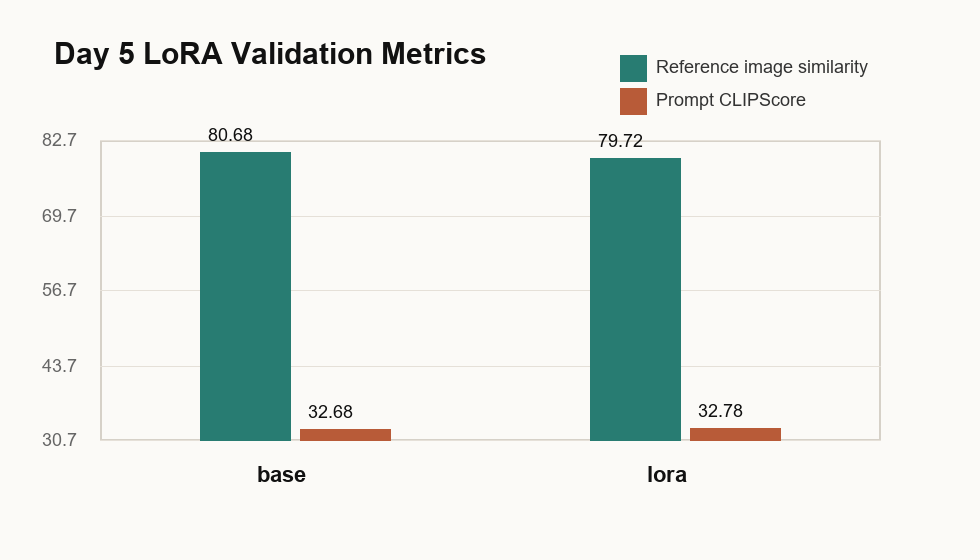
\includegraphics[width=\linewidth]{day5_lora_validation_scale1_metrics.png}
    \caption{LoRA scale=1.0}
  \end{subfigure}
  \hfill
  \begin{subfigure}{0.48\linewidth}
    \centering
    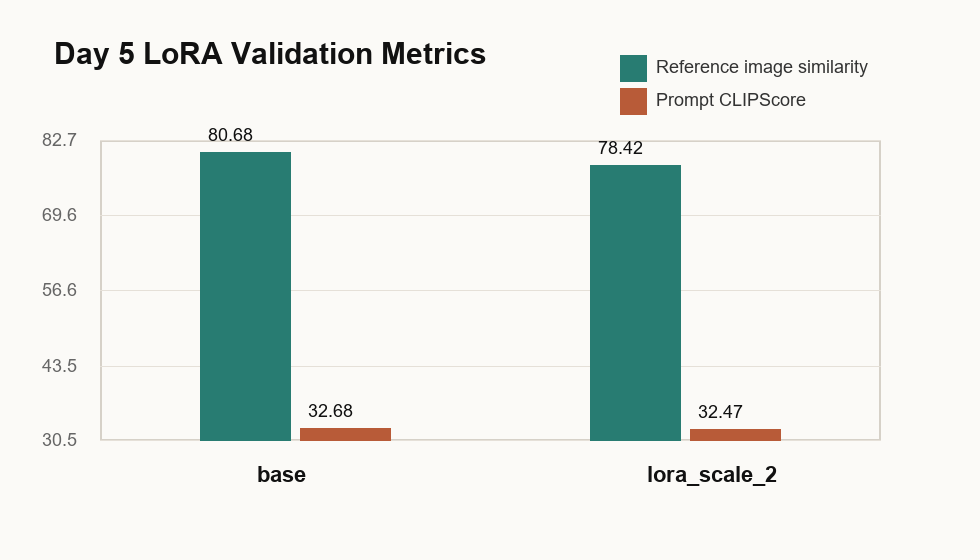
\includegraphics[width=\linewidth]{day5_lora_validation_scale2_metrics.png}
    \caption{LoRA scale=2.0}
  \end{subfigure}
  \caption{LoRA 初始验证的自动指标图。}
  \label{fig:appendix_lora_metrics}
\end{figure}

\end{document}
